\documentclass[12pt]{report}
\usepackage[utf8]{inputenc}
\usepackage[paper=a4paper,pdftex,top=3cm,left=2.5cm,right=2.5cm,foot=1cm,bottom=3cm]{geometry}
\usepackage{graphicx} %Graphics package for \includegraphics
\usepackage{caption}
\usepackage{subcaption}
\usepackage{wrapfig} %Enables wrapping of text around figures and tables
\usepackage{subfig}
\usepackage{enumerate}
\usepackage{placeins}
\usepackage{SIunits}%SI unit symbol package
\usepackage{amsmath}
\usepackage{array, calc}
\usepackage{cite}
\usepackage{mathtools}
\usepackage{fontenc}
% \usepackage{picinpar}
% \usepackage{multirow}
% \usepackage{tabularx}
% \usepackage{setspace}
% \usepackage{verbatim} %Enables \begin{comment}...
% \usepackage{float}
% \usepackage{threeparttable}
% \usepackage{standalone}
% \usepackage{booktabs, dcolumn}
% \usepackage{fancyvrb}
\usepackage[printonlyused]{acronym}
\usepackage[titletoc]{appendix}

\numberwithin{figure}{chapter}
\setcounter{secnumdepth}{3}

\tolerance = 5000 % LaTeX er normalt streng n�r det gjelder linjebrytingen.
\hbadness = \tolerance % Vi vil v�re litt mildere, s�rlig fordi norsk har s�
\pretolerance = 2000 % mange lange sammensatte ord.


% \usepackage{afterpage}
% \newcommand\blankpage{%
%     \null
%     \thispagestyle{empty}%
%     \addtocounter{page}{-1}%
%     \newpage}


%\newenvironment{packed_enum}{
%\newenvironment{enumerate}{
%\begin{enumerate}
%   \setlength{\itemsep}{10cm}
  \setlength{\parskip}{18pt}
%   \setlength{\columnsep}{3cm} 
%   \setlength{\parsep}{10pt}
%}{\end{enumerate}}


% \usepackage{nomencl}
% \makenomenclature
% \renewcommand{\nomname}{Abbreviations}


\providecommand{\e}[1]{\ensuremath{\times 10^{#1}}}

\usepackage[hidelinks]{hyperref}

\begin{document}

%Forside
\thispagestyle{empty}
\begin{center}        
  \vspace{5mm}        
  \huge
  \textbf{Radiation Testing of RCU2 Components} \\
  \vspace{50mm}
  \Large
  {\bf{\textsl{Inge Nikolai Torsvik}}} \\
  %\textsl{Eksperimentalfysikk med prosjektoppgave} \\
  \vspace{20mm}
  %{\bf{\textsl{Oppgave 12}}} \\
  \vspace{5mm}
  %{\large \textsl {(Bachelor i Fysikk)}}\\
  \vspace{10mm}
  \centerline{\includegraphics[height=4cm,width=4cm]{figures/uglo}}
  \Large
  \textsl{Master Thesis} \\
  \vspace{45mm}
  \large
  \textsl{Department of Physics and Technology} \\
  \textsl{University of Bergen} \\
  \vspace{10mm}
  \large
  \textsl{June 2014} \\

\end{center}

%\thispagestyle{empty}


\setcounter{page}{1}
\pagenumbering{Roman}

\chapter*{Acknowledgements}


\chapter*{Abstract}
At CERN in Switzerland the largest particle accelerator ever built called \ac{LHC} is located. The LHC is placed 100 meter below ground level in a 27 km long tunnel where four experiment areas are located, one of these experiment is \ac{ALICE}. \ac{ALICE} is built to study a matter known as Quark-gluons plasma, which will be generated under collisions of heavy ions. LHC is currently shutdown for maintenance and preparation for even higher energies. This period called Long Shutdown 1 (LS1), started January 2013 and will last until the end of 2014.

ALICE comprises of several sub-detectors, one of these are \ac{TPC}, which is the main tracking device of ALICE. For LS1 it has been decided that a upgrade should be performed on the \ac{RCU}, which controls the readout in the TPC. The new RCU, named RCU2, will increase the present readout rate by a factor of up to 2.6, and will be more immune to radiation induced errors.

For the RCU2 design new components are introduces, where some of these hasn't been tested for radiation tolerance. The work presented through this thesis comprises of irradiation tests of these components. The tested components consist of power regulators, bus transceivers, limiting amplifier, multiplexer/demultiplexer, buffer, comparator, Current Shunt Monitor and the RCU2's main FPGA, the Microsemi \ac{SF2}. The tests performed consist mostly of test for accumulative effects, but test for \ac{SEE} will also be performed for some of the components.

The main focus has been on the SF2 SoC FPGA, where test of \acl{SEE} like \ac{SEU}, \ac{SET} and \ac{SEL} has been executed on SRAM, logic element and PLL.

The irradiation tests has been executed at \ac{OCL} in Oslo Norway, with a proton beam of 25 and 28 MeV and at \ac{TSL} in Uppsala Sweden, with a proton beam of 170 MeV.

\tableofcontents



\chapter{Introduction}
\setcounter{page}{1}
\pagenumbering{arabic}
At \ac{CERN} in Switzerland there are being conducted experiments on fundamental structure of the universe. This is done by accelerating particles up to an energy level of 4 $\tera \electronvolt$ per proton, and then colliding them with other particles on the same energy level. The largest accelerator is called \acf{LHC}, and is the largest particle accelerator ever built, installed in a 27 $\kilo \meter$ long tunnel.
Particles are accelerated in both directions in the LHC. When the particles have reached high enough energy, particles from the opposite directions are made to collide at 4 experiment areas, one of these is called \ac{ALICE}.
\ac{ALICE} is built to study a matter known as Quark-gluons plasma , which will be generated under collisions of heavy ions \cite{ALICE}.
ALICE consists of several sub-detectors with different functionalities. \ac{TPC} is one of these, and is the main tracking detector placed closest to the beam-line, see \autoref{ALICE_experiment}. Under a collision, high energy particles will be generated, which will also pose a risk to the electronics used.
It is therefore of highest importance to test everything that is planned to be used in the experiment for radiation.

SKRIV NOE OM OPPGGRADERINGEN I LHC (RUN2,RCU2?,LS1)

One of the main boards used in the \ac{TPC} detector is the \acf{RCU}. It has been decided that a new \ac{RCU} shall be made, named RCU2.
Because of the radiation level in the \ac{LHC}, every component used in the design of the RCU2 has to be tested for radiation to be sure that it won't fail when it is installed in the \ac{TPC} detector.

\section{How to Test}
\label{how_to_test}
The radiation tests performed through this work are mainly tests for accumulative effects.
Accumulative effects are effects caused by the total radiation of a component, and are measured by the functionality and power consumption of the component, see \autoref{accumulative_sec} for more information.

Test for \acf{SEE} like \acf{SEU}, \acf{SET} and \acf{SEL} on a Microsemi \ac{SF2} \ac{SoC} \ac{FPGA} have also been performed.

Research has previous been performed on the radiation level in the \ac{ALICE} \ac{TPC} \cite{Safarik} and \cite{georgios}, and is used to decide if the tested components can be used or not.

\section{About This Work}
I started working on the RCU2-project in the autumn of 2013. Already before I started working, the design and the schematic layout for the RCU2 was basically finished. In the design process components that already were tested or are proven to be radiation tolerant were used when possible, but such components weren't always available. Therefore my work in this project has been to do irradiation tests on components for the RCU2 design which didn't have any record of being tested for radiation.

The components which I have tested are: TPS51200, MIC69302WU, SN74AVCB164245, SN74AVC2T245, QS3VH257, SY89831, ADN2814, TLV3011 and SF2-M2S050-FG896. These components consist of: power regulators, bus transceivers, limiting amplifier, multiplexer/demultiplexer, buffer, comparator, Current Shunt Monitor and  \ac{SoC} \ac{FPGA}.
In order to investigate the radiation tolerance of these circuits I had to first acquire good knowledge of radiation induced effect that may occur in such devices. I also needed to study the components to be able to find a reasonable test methodology. Further, I had to familiarize myself with CAD tools such as \emph{expedition PCB} and \emph{DXdesigner} and programming and developing environments like Libero and LabVIEW in order to develop a sufficient hardware and software based test setup for the components.

The RCU2's main FPGA the Microsemi \ac{SF2}, has been the main focus through this work. This is because the component will be hard to replace, and a functional failure on this one may set the whole RCU2 out of function. The radiation effects that were tested on for \ac{SF2} are SRAM blocks for SEU, logic elements for SEU and SET, and in general SEL. These effects can be read about in \autoref{SEE_section}.

The irradiation tests were executed in four periods; three times at \ac{OCL} with a proton beam of 28 MeV and 25 MeV, and one time at \ac{TSL} with a proton beam of 170 MeV. 
% A \ac{SF2} starter-kit was used when designing test for this component, and test code was written in VHDL and C. To be able to detect SEL the current on the FPGA had to be measured. Therefore a current measurement board was made for that task.

To summarize, this work has been consisting of practical work like making \acp{PCB}, writing test code in VHDL, making LabVIEW programs and making test codes in C. It has also included getting the necessary knowledge of the components tested, learning to program in VHDL and C, as well as learning to use the tools and programs for the different tasks. And of course setting up test setup, and irradiate the components.

\newpage

\chapter{ALICE Experiment}
\label{ALICE_experiment}
Since 1954 physicists at \ac{CERN} have studied the nucleus and its structure to find the fundamental structure of the universe.
\acs{CERN} is the world largest research center for nuclear and particle physics, and has a total of 21 member states.
One of the biggest attractions at \ac{CERN} is the \acf{LHC}, which is a circular particle accelerator placed in a 27 km long tunnel around 100 meters beneath ground level.
This is the last accelerator in a chain of up to 7 (depending on which particle to accelerate), see \autoref{CERN_accelerators}, where the particles gradually accelerate to higher and higher energies, up to their maximum energy of 4 TeV and speed close to the speed of light. When particles have reached this energy level accelerated particles from opposite directions are made to collide inside 4 different experiment areas, where one of these is called \acf{ALICE}, see \autoref{ALICE_layout}.

The main purpose of ALICE is to study a state of matter called quark-gluon plasma which will be generated when heavy ions collides.
Under these collisions a temperature 100 000 times higher than the temperature of the sun is generated.
There is then high enough energy to split the protons and neutrons, and achieve a plasma of unbound quarks and gluons, and that is whats called quark-gluon plasma.

All ordinary matter in today's universe is made up of atoms.
Each atom contains a nucleus composed of protons and neutrons (except hydrogen, which has no neutrons), surrounded by a cloud of electrons.
Protons and neutrons are in turn made of quarks bound together by other particles called gluons.
No quark has ever been observed in isolation: the quarks, as well as the gluons, seem to be bound permanently together and confined inside composite particles, such as protons and neutrons.

\begin{figure}[!htbp]
  \centering
  \includegraphics[width=0.60\textwidth]{figures/CERN_accelerators}
  \caption{CERN accelerators \cite{website:CERN_accelerators}}
  \label{CERN_accelerators}
\end{figure}

\begin{figure}[!htbp]
  \centering
  \includegraphics[width=\textwidth]{figures/ALICE_layout}
  \caption{Layout of the ALICE experiment \cite{website:aliceinfo}}
  \label{ALICE_layout}
\end{figure}

\FloatBarrier

\section{The Time Projection Chamber TPC}
The ALICE detector comprises of several sub-detectors, where one of these is the \acf{TPC}. The \ac{TPC} is the main tracking detector of \ac{ALICE}.
The functions of \ac{TPC} are tracking particles, measure the charged particles momentum and identification of particles.
A drawing of the \ac{TPC} can be seen in \autoref{TPC_layout}.
The \ac{TPC} detector has a cylindrical shape, with an inner radius of 85 cm and outer radius of 250 cm, and has an overall length of 510 cm.
The detector is made up of a large cylindrical field cage, filled with 88 $m^3$ of 90\% Ne gas and 10\% $CO^2$ gas.
A high voltage electrode is placed in the center of the detector, dividing the \ac{TPC} into two drift regions, and making an electric field between the electrode and the two end plates.
When a charged particle is generated inside the detector, the gas inside the cage will be ionized. The free electrons and the ions will then drift in the electric field between the high voltage electrode and the two end plates.
At the end-plates the Readout Chamber is located, which is divided into 18 trapezoidal sectors, where each sector is again divided into the inner and outer chamber.
In the readout chamber, there are a total of 560 000 readout pads.

\begin{figure}[!htbp]
  \centering
  \includegraphics[width=\textwidth]{figures/TPC_layout}
  \caption{Layout of the TPC \cite{website:aliceinfo}}
  \label{TPC_layout}
\end{figure}

\newpage

\begin{wrapfigure}{r}{0.5\textwidth} 
\vspace{-40pt}
  \begin{center}
  \includegraphics[width=0.5\textwidth]{figures/TPC_Sections}
  \caption{A TPC sector, showing distribution of FECs \cite{roed_doctor}}
  \label{TPC_Sections}
  \end{center}
  \vspace{-80pt}
\end{wrapfigure}

\section{The TPC Front End electronics FEE}
Each of the 36 sections (2 x 18) are also divided into 6 readout partitions; 2 in the inner chamber and 4 in the outer chamber.
There are a total of 216 \ac{RCU} connected to a total of 4356 \ac{FEC} which are connected to all of the 560 000 readout pads, and all together this sums up the \acf{FEE}, see \autoref{TPC_Sections}. In short, the task of the \ac{FEE} is to read out the charge received at the readout pads, process it and send useful data to a computer.



\FloatBarrier
\subsection{Front End Card FEC}
A current signal given by one of the pads, is sent into a \acf{FEC} which consist of three basic functional units, see block diagram in \autoref{FEC_blockdiagram}.
The first unit is a charge sensitive amplifier/shaper called PASA, the second unit is a 10-bit 10 MHz low-power \ac{ADC}, and the last unit is a digital circuit that performs the baseline subtraction, tail cancellation, zero-suppression\footnotemark, formatting, and buffering.
The \ac{ADC} and the digital unit together constitute the so called ALTRO chip. There are 16 PASA chips and 16 ALTRO chips on the \ac{FEC},
the PASA chip is connected to 16 readout pads each, which gives a total of 128 readout pads for each \ac{FEC}.


\begin{figure}[!htbp]
  \centering
  \includegraphics[width=\textwidth]{figures/FEC_blockdiagram}
  \caption{Block diagram of the Front End Card \cite{website:aliceinfo}}
  \label{FEC_blockdiagram}
\end{figure}

% \begin{figure}[!htbp]
%   \centering
%   \includegraphics[width=0.7\textwidth]{figures/FEC}
%   \caption{Top side of the Front End Card \cite{roed_doctor}}
%   \label{FEC}
% \end{figure}

\footnotetext{Zero Compressions means that signal below a given threshold will be filtered away.}
\FloatBarrier
\subsection{Readout Control Unit RCU}
One \acf{RCU} is connected to one row of \acp{FEC} (up to 25 pieces), through a backplane\footnotemark, see \autoref{TPC_Sections}.
The \ac{RCU} task is to control the entire \acf{FEE} all the way from the readout pads through the \acp{FEC}, and out to a \acf{DAQ} System.
The \ac{RCU} consist of three separated boards which are the Motherboard board, the \acf{DCS} board, and the \acf{SIU} board.
Most of the \ac{RCU} functions are controlled by the Xilinx Virtex-II Pro \ac{FPGA}.
This \ac{FPGA} are controlling the readout process of the \ac{TPC} detector.
It is also responsible for moving data from the \acp{FEC} to the \acf{SIU} board,
where data is transmitted via an optical link to the Data Acquisition system.
In the Data Acquisition system data is stored and is accessible for analysis.

\begin{wrapfigure}{r}{0.6\textwidth} 
\vspace{-20pt}
  \begin{center}
  \includegraphics[width=0.6\textwidth]{figures/RCU}
  \caption{The Readout Control Unit top side and bottom side \cite{roed_doctor}}
  \label{RCU}
  \end{center}
  \vspace{-30pt}
\end{wrapfigure} 

The Xilinx Virtex-II Pro is a \ac{SRAM} based \ac{FPGA}. \ac{SRAM} cells are vulnerable for \acfp{SEU}, see \autoref{SEU_Section}.
Therefore a flash based \ac{FPGA}, Actel ProASIC is used to monitor the SRAM memory and reprogram/reconfigure if an error occurs.

The \ac{DCS} board is basically an embedded computer running Linux.
This board is connected through an Ethernet link to a computer on the outside of the ALICE detector.
Through this it is possible to upgrade and reprogram the \acp{FPGA} of the \ac{RCU}.
So even though the hardware is inaccessible after it has been mounted in the \ac{TPC},
the \ac{SIU} boards gives some kind of flexibility.
In addition, it has an optical interface, receiving the clock and trigger information from the Timing, Trigger and Control system, also called TTC.


\footnotetext{A backplane is a PCB board, that connects Front End Cards to a Readout Control Unit.
This is used instead of cables to get a more stability, and to keep things in place.}

In \autoref{FEE_overview} you can see a full overview of the \ac{RCU} and its connections.

\begin{figure}[!htbp]
  \centering
  \includegraphics[width=0.8\textwidth]{figures/FEE_overview}
  \caption[FEE overview]{The architecture and readout path of the TPC electronics for one readout partition \cite{roed_doctor}.}
  \label{FEE_overview}
\end{figure}


\subsection{RCU2}
\subsubsection{Why Upgrade RCU} 
LHC is currently shutdown for maintenance and preparation for even higher energies.
This period, called Long Shutdown 1 (LS1), lasts until end of 2014.
The present \ac{TPC} readout electronics will be a limiting factor with the foreseen readout rate for the next run period (run2) \cite{RCU2}.
The bus between \ac{RCU} and FECs is not able to read all data for high occupancy events, like Pb-Pb collisions.  
In addition stability issues related to \ac{SEU} on the \ac{SRAM} based \ac{FPGA} have been observed with the present setup.
9 \% of the run time had to be stopped because of errors in the \ac{TPC} readout electronics.

\subsubsection{The new Readout Control Unit, the RCU2} 
The main challenge making the RCU2 was to develop a solution that gives the needed performance improvement,
and at the same time was feasible within the limited time-frame.
Therefore some of the old infrastructure has to be reused, like cables for Ethernet, Trigger and power and the cooling envelops.
RCU2 will increase the present readout rate by a factor of up to 2.6, and will be more immune to radiation induced errors.

The main difference between the RCU2 and \ac{RCU}1 is that the main \ac{FPGA}, the Xilinx Virtex-II Pro,
has been replaced by a Microsemi \acf{SF2} \acf{SoC} \ac{FPGA} M2S050-FG896. This is a flash-based\footnote{Flash-based FPGA means that configuration registers is saved in flash memory cells. Compared to SRAM-based FPGA where configuration is saved in SRAM cells, flash-based FPGA is much more tolerant against radiation.}
FPGA which has \ac{SEU} immune configuration memory, as well as several other radiation tolerance measures implemented \cite{website:SF2_datasheet}.
It also comes with a Microcontroller Subsystem which is based on a hardcore ARM Cortex-M3 microcontroller.
On the Microcontroller Subsystem a Linux system can be built, which replaces the functionality of the \ac{DCS}-card.
The ProASIC was also not needed as a  reconfiguration FPGA anymore, but will still be used as a radiation monitor.
This part of the RCU2 is now called RadMon, and consists of a ProASIC and SRAM chips.
The TTCrx chip that was used for handling the clock and trigger signal on RCU1 was out of stock and obsolete, and will be replaced by an optical receiver and a limiting amplifier. The limiting amplifier has been tested in the work presented in this thesis, see \autoref{limiting_amp}.

One of the limits with the old setup was that the bus between \ac{RCU} and FECs was to slow, especially after the upgrade in the \ac{LHC} for run2.
This was fixed by dividing the readout into 4 sections instead of 2, which effectively doubled the readout speed.
Therefore all of the backplanes had to be redesigned and replaced.

\FloatBarrier
\newpage


\chapter{Radiation and Radiation effect on Semiconductor Devices}
Radiation and radiation induced effects are known challenges when designing electronics which is going to be used in the LHC.
It is therefore of highest importance to know about these effects, how they affect the electronics, how much damage they can cause and how to protect and prevent the radiation effects to do damage.

This chapter is based on references \cite{rad_phys}, \cite{CMOS}, \cite{knoll}, \cite{Baumann} and \cite{balashov} if not otherwise stated.

\section{Interaction of Radiation with Matter}
Radiation is defined as a process in which energy in the form of energetic particles or electromagnetic waves are transmitted through a medium or space.
Radiation is normally divided into two categories, namely \emph{Charged radiation} and \emph{Neutral radiation}.

Charged radiation consist of charged particles like protons (p), alpha ($\alpha$) and beta ($\beta$) particles and heavier ions.
Neutral radiation consist of neutral particles like neutrons (n) and photons from gamma ($\gamma$) and X-rays. 
Particles which interact with a material will deposit some or all of its energy in the interaction, and can either interact with atoms, electrons, nucleus or the particles inside a nuclei.
How much energy is deposited, and which of these a particle will interact with, depends on the energy, mass, the charge of the particle and what material it interacts with.
One of the main differences between charged particle and neutral particle is that charged particles will be affected by the Coulomb force,
which is the attraction or repulsion of particles or objects due to their electric charge.
In the following sections we will look more closely into how a charged particle and neutral particle interact with matters.
%It is common to distinguish between Ionizing and non-ionizing radiation.
%Ionizing radiation consist of particles with high enough energies so that they can detach electrons from an atom or molecule and ionize them.
%Non-ionizing radiation is than obviously radiation of particles with energies to low to ionize a atom or molecule.

\section{Charge particle and their Interaction with Matters}
\label{radiation_phys}
When a charged particle with high speed is passing through a material it will experience multiple elastic and inelastic collisions with the atoms in that material, resulting in slowing down or stopping the particle.
When a particle collides with an atom there are several processes that can contribute to the loss of energy. They are:

\begin{itemize}
  \item Inelastic scattering towards atomic electrons \hfill
  \begin{itemize}
    \item Excitation and ionization
  \end{itemize}
  \item Elastic scattering towards atomic electrons \hfill
  \begin{itemize}
  \item Ramsauer Effect
  \end{itemize}
  \item Inelastic scattering towards Nuclei \hfill
  \begin{itemize}
  \item Nuclear reaction
  \end{itemize}
  \item Elastic scattering towards Nuclei  \hfill
  \begin{itemize}
  \item Rutherford/Nuclear scattering
  \end{itemize}
  \item Other processes \hfill
  \begin{itemize}
  \item Bremsstrahlung and Cherenkov radiation
  \end{itemize}
\end{itemize}

Which of these processes that contributes most to the loss of energy depends on the initial energy, velocity, mass and charge of the particle as well as the properties of the material it collides with.
For example, for heavy charge particles (protons or heavier ions), inelastic collisions with the atomic electrons in a material will contribute to most to the energy loss of the particle.
A common expression for these processes is called "stopping power".

\subsection{Stopping Power}
If a particle with a given energy passing into a material, where $dE$ is the mean energy that the particle loses by traveling through a path segment, $dx$ of the material.
Then $-\frac{dE}{dx}$ is the stopping power or also called the "rate" of energy loss for the particle.
The stopping power depends on the type and energy of the radiation and on the properties of the material it passes.

The classical expression that describe the stopping power is the \emph{Bethe Bloch formula}, and is written in \autoref{stopping_power}.

\begin{equation}
S = - \frac{dE}{dx} = \frac{n_A Z_A Z^2 e^4}{4 \pi \epsilon_o m_e V^2}\Bigg[\ln\Big(\frac{2 m_e \upsilon^2}{\overline{I}}\Big)-\ln\Big(1-\frac{\upsilon^2}{c^2}\Big)-\frac{\upsilon^2}{c^2}\Bigg]
\label{stopping_power}
\end{equation}

\begin{table}[!htbp]
\begin{tabular*}{0.6\textwidth}{@{\extracolsep{\fill} } l l }
$n_A$ & Number of atoms per unit volume \\
$Z_A$ & Average atomic number of the material \\
$Z$ & Atomic number of particle \\
$e$ &  Electron charge \\ 
$c$ &  Speed of light \\ 
$\epsilon_o$  & Vacuum Permittivity \\
$m_e$ &  Electron rest mass \\ 
$\upsilon$  & Particle velocity \\
$\overline{I}$ & Effective material ionization potential \\
\end{tabular*}
\label{bethe_bloch}
\end{table}

% \subsection{Specific Stopping Power}
% Another way of looking at stopping power is by looking at energy loss as function of mass per area $-\frac{dE}{d\xi}$.
% Here $\xi$ = $\rho$x and $\rho$ is the density of the material. The unit for specific stopping power is given as $[\frac{\mega\electronvolt\centi\meter^2}{\gram}]$
% 
% \begin{equation}
% S = - \frac{dE}{d\xi} = - \frac{1}{\rho} \frac{dE}{dx} 
% % = - \frac{n_A Z_A Z^2 e^4}{4 \pi \epsilon_0^2 m_e \upsilon^2}\Bigg[\ln\Big(\frac{2 m_e \upsilon^2}{\overline{I}}\Big)-\ln\Big(1-\frac{\upsilon^2}{c^2}\Big)-\frac{\upsilon^2}{c^2}\Bigg]
% \label{sstopping_power}
% \end{equation}

From this formula, if considering two different particles with the same velocity, the only factor that changes is $Z^2$.
Therefore heavier particles will experience larger energy loss in a material compared to lighter ones.
\autoref{energy_loss} shows energy loss for different particles in air.
The value of $\frac{dE}{dx}$ for different types of particles approaches a near-constant broad minimum value at energies above several hundred $\mega\electronvolt$, where their velocity approaches the velocity of light.

\begin{figure}[!htbp]
  \centering
  \includegraphics[width=0.5\textwidth]{figures/energy_loss}
  \caption[Energy loss in air]{Variation of the specific energy loss in air versus energy for different particles \cite{rad_phys}}
  \label{energy_loss}
\end{figure}
\FloatBarrier

% At low particle energy, where charge exchange between a particle and a absorber becomes important, the Bethe Bloch formula begins to fail.
% This happens because the positively charged particle in this case tend to pick up electrons from the absorber, which effectively reduce its charge and consequently linear energy loss, and will at the end become a neutral atom.

\subsection{Linear Energy Transfer LET}
\label{LET_section}
\acf{LET} is closely related to stopping power of a particle, but instead of focusing on energy loss of the particle, \ac{LET} focuses on the energy that is deposited to a material in a local volume.
For low energies, \ac{LET} is often said to be equal to the stopping power, even though the particle energy that turns into photons may escape the local area.
For higher energies, small particles like ionized electrons can escape the local volume. The local volume is defined by the user,
and can be everything from part of a molecule to a whole organ.
One alternate definition of LET can be seen in equation \ref{LET},

\begin{equation}
L_\Delta= \bigg(- \frac{dE}{dx}\bigg)_\Delta
\label{LET}
\end{equation}

where $\Delta$ is the upper energy limit for the secondary electrons included in the calculations.
If $\Delta$ is set to $\infty$, all secondary electrons are included in the calculations, making \ac{LET} the same as stopping power.

\section{Neutral particle and their Interaction with Matters}
\subsection{Neutrons}
Neutrons are subatomic structures that are present in most atomic nuclei.
Neutrons carry no charge and can therefore not interact with matter by means of the Coulomb force,
which dominates the energy loss mechanisms for charged particles.
Neutrons can also penetrate several centimeters into matters without any type of interactions, making neutrons hard to detect.
When neutrons undergo an interaction it is with the nucleus of the absorbing material.
This can result in total disappearance of the neutron creating one or more secondary radiations, or change of the direction of the neutron.  
The secondary radiations from neutrons are largely ionizing.

\subsection{Photons}
Photons may appear from gamma rays or X-rays. Photons have as neutrons no charge, and are therefore not affected by the Coulomb force, additionally photons have no rest mass and travel in constant speed of light.
The energy of a photon is given in the formula $E=hf$ where f is the frequency of the particle and h is the Planck`s constant.
There are three main processes where a photon may react with matters, they are: Photo electric effects, Compton scattering and Pair production.

\section{Radiation Effects on Semiconductor Devices}
Semiconductor devices planned to be used in a radiation environment are likely to be effected by the radiation in some way.
If not taken properly into account, the radiation effects may damage or even destroy the electronics.
Therefore it is of highest importance to know how irradiation can affect the semiconductor devices.
Normally radiation effects are divided into two groups; $\emph{Singel Events effects}$ and $\emph{Accumulative Effects}$.

\subsection{Single Events Effects SEE}
\label{SEE_section}
\acf{SEE} happens due to the energy deposited by one single particle in a electronic device. 

These effects can happen in any moment under radiation, and their probability is expressed in terms of cross section\footnotemark \cite{website:Faccio}.
These effects have been an increasing problem as the manufacture processes are getting smaller and smaller.
In the following sections the three most known \ac{SEE} will be looked into. These are \acf{SEL}, \acf{SET} and \acf{SEU}.

\footnotetext{Cross section is the probability that an incoming particle will induce a single event effect, and is expressed in $\centi\meter^2$}
\subsubsection{Single Event Latchup SEL} 
A \acf{SEL} is a phenomenon where a low resistance path between power and ground is formed, causing large current to flow. Normally latches will cause burned interconnections, which means reduced performance or destruction of the chip. \ac{SEL} can be discovered by measuring current of a chip, and can be seen as large jumps in current. The only way to counter a latchup is by turning power off, and that is before the high current will burn interconnections and permanently set the chip out of function.

%Since the consequences is so severe, it is of highest importance to know about this effect, and know how to counter or to protect from latches in design phase. 

How a latchup may occur can be understood by looking at a CMOS inverter, see \autoref{CMOS_inverter}.
\autoref{CMOS_inverter}(a) shows a parasitic bipolar npn-transistor and pnp-transistor formed inside the inverter, and a resistor formed in the well and substrate. An equivalent circuit can be seen in \autoref{CMOS_inverter}(b).
Originally both of the bipolar transistors are turned off, and no current flows through the transistors.
A latchup can be triggered if an ionizing particle flows into the substrate creating a transient current that can set $V_{sub}$ high, causing npn-transistor to turn ON.
If the npn-transistor turns ON, then current will flow through $R_{well}$ causing $V_{well}$ to go low and setting the pnp-transistor ON.
When the pnp-transistor turns ON current will flow through $R_{sub}$, causing $V_{sub}$ to rise, and a positive feedback is created, causing high current to flow from power to ground.

\begin{figure}[!htbp]
  \centering
  \includegraphics[width=\textwidth]{figures/CMOS_inverter}
  \caption[CMOS inverter]{(a) A CMOS inverter with parasitic bipolar transistors (b) A model of the parasitic circuit \cite{CMOS}}
  \label{CMOS_inverter}
\end{figure}

\subsubsection{Single Event Transient SET} 
\label{SET}
\acf{SET} is a transient pulse of current in a logical path of a circuit.
A \ac{SET} is caused by an ionizing particle which travels through a material, leaving a transient current pulse on a track or node in an circuit.
If a transient occurs close or on a sensitive circuit node like the input signal to a register, the transient can cause a short period of changed value on input node. If the clock signal to that register goes high exactly when the transient happens, it can cause an unwanted change of value on the output of the register, which is called a \ac{SEU}.
If the transient is not clocked out or saved in some way, the current peak will just flat out, and will probably not be detected or cause any damage.
Since \acp{SET} are close to impossible to detect, SET is measured in terms of SEU.

\subsubsection{Single Event Upset SEU} 
\label{SEU_Section}
\acf{SEU} is change of state in a logical element, caused by radiation. This phenomenon can often be seen in memory cells or registers, where data is stored.
A \ac{SEU} is a "Soft error", which means that it is a non-destructive type of error. By resetting or overwriting after an \ac{SEU} has occurred, the error will disappear.

For better understanding of \ac{SEU} a six transistor SRAM cell will be explored, see \autoref{SRAM_Cell}. If starting with Q = '0' and Q\_b = '1', which means that there is a value '0' written to the cell.
Then a high energetic neutron strikes into the drain of transistor D\_2 and hits a silicon atom, which causes shattering of the atom into charged fragments (ions) that travel through the substrate.
These ions leave a trail of electron-hole pairs, see \autoref{charge_generation}(a).
When the resultant ionization track traverses or comes close to the depletion region,
carriers (electrons) are rapidly collected by the electric field creating a large current transient at that node, causing a voltage drop at node Q\_b.
If this voltage drop is high enough, transistor P1 will be opened, and transistor D1 will be closed, causing Q to be charged towards '1'. When Q goes towards '1' transistor P2 will be closed and transistor D2 will be open, causing Q\_b to be discharged through D2, and fall towards '0'. The SRAM cell has then got a unwanted change of value from '0' to '1', and that is called a \ac{SEU}.

\begin{figure}[!htbp]
  \centering
  \includegraphics[width=0.75\textwidth]{figures/SRAM_Cell}
  \caption{Six transistor SRAM Cell \cite{CMOS}}
  \label{SRAM_Cell}
\end{figure}

\begin{figure}[!htbp]
  \centering
  \includegraphics[width=\textwidth]{figures/charge_generation}
  \caption[Principle of Charge Generation]{(a) Electron hole pairs generated (b) Carrier are drawn towards the depletion region causing a current jump (c) Additional charge is collected on a more long time scale (hundreds of nanoseconds) \cite{Baumann}}
  \label{charge_generation}
\end{figure}

\FloatBarrier

\subsection{Accumulative Effects}
\label{accumulative_sec}
Accumulative effects are energy deposition caused by radiation for the whole lifespan of a circuit \cite{website:Faccio}, \cite{Oldham}.
Accumulative effects are measured by the functionality of a device, and power consumption. 
Some circuits are weak for accumulative effects, and will stop working only after a small dose of radiation,
but other devices may not even have any effect after a severe dose of radiation. When a chip stops working, it has reached its tolerance level.
Talking about accumulative effects it is normal to divide into two groups; displacement damage, which is a non-ionizing effect
and \ac{TID}, which is an ionizing effect.


\subsubsection{Total Ionization Dose TID} 
\label{TID}
\acf{TID} is a measurement of the energy deposited in a circuit by radiation in the form of ionization energy.
The units used are Gray (\gray) or rad. The relation between those two can be seen in equation \ref{gray_rad}.

\begin{equation}
1 \gray = 100 \rad
\label{gray_rad}
\end{equation}

The heart of \ac{TID} effects is the energy deposition in the silicon dioxide.
When ionizing particles penetrate into a transistor, electron-hole pairs will be created.
Most of the pairs will recombine shortly after they are generated, but some do not completely recombine because of the electric field.
Electrons, with high mobility, can easily leave the oxide, but holes have lower mobility and can be trapped in their point of generation in the oxide.
The trapped holes cause a negative threshold voltage shift in the MOS transistor, and if enough holes are trapped, it can result in a transistor which is permanently ON.
This phenomenon can be seen in \autoref{TID_in_MOS}.

One effect of the total ionized dose in CMOS circuits is increase in current, which could be caused by threshold change in transistors. An example with an inverter can be looked at. An inverter consist of only a PMOS and a NMOS, if threshold decreases, time where both transistors are on will increase, leading to increase of current. Another reason for current increase is current leakage between drain and source because of trapped holes.

\begin{figure}[!htbp]
  \centering
  \includegraphics[width=0.5\textwidth]{figures/TID_in_MOS}
  \caption[MOS transistor under radiation]{Layout of a MOS transistor. (A) Shows normal operation and (B) shows the transistor after irradiation. \cite{roed_doctor}}
  \label{TID_in_MOS}
\end{figure}

\subsubsection{Displacement Damage} 
Displacement Damage is a non-ionizing effect mostly induced by low energetic particles colliding with and breaking atoms out of the initial lattice structure of a material.
This can affect the functionality of the device. CMOS circuits are normally considered immune to this effect. 
Displacement damage is not measured in any unit, but it is expressed in terms of the particle fluence, in particles/$\centi\meter^2$.

\subsection{The TPC Radiation Environment}
\label{TPC_environment}
Radiation in the \ac{LHC} is dominated by high energetic neutrons and protons, mostly neutrons with an estimated fluence of $(0,6-1,1)\times 10^{11}$ $neutrons/cm^2$ \cite{georgios}.
Therefore it would be preferable to test our electronics with a neutron beam, but since there are few labs that can produce a neutron beam compared to proton beam most of the electronics are only tested at \ac{OCL} with a proton beam.
There has been conducted experiments that compares SEU induced by neutrons and protons \cite{GranlundOlsson}, and the results shows that it is possible to use a proton beam instead of neutron beam with small deviations.
By comparing a proton beam with a neutron beam of 21 MeV there are 10-25\% less \ac{SEU} cross section for a proton beam compared to a neutron beam.
If the energy is increased to 88 MeV there is close to no deviation. 

Several calculations has been done on the present radiation level in ALICE \cite{georgios} and \cite{radiation_alice}. From these calculations it is expected a high energy hadron fluence rate ($>20MeV$) of 0.8 kHz/cm2, and that is for the worst case location of the TPC electronics, and for an interaction rate of 8 kHz. Scaling this fluence rate to an interaction rate of 30 kHz, the expected value for Run2 becomes 3 kHz/cm2 , which is a significant rate. For run1 a total dose and 1 MeV neutron-equivalent fluence was estimated to be 1.6 kRad and $4.5\cdot10^{10} \centi\meter^-{2}$ respectively, and this for a total operation of 10 ALICE years. If assuming a similar run program of p-p, p-Pb and Pb-Pb interactions, and then scaling for a 3 year running period of Run2 including an increased interaction rate of 30 kHz for Pb-Pb, a similar dose of around 1-2 $\kilo$Rad and a fluence in the order of $10^{10}$ could be expected for run2.

%Section about what our electronics will receive at CERN

\FloatBarrier
\newpage

\chapter{Preparations for Radiation Testing}
Testing components is a process that has been done many times before in conjunction with design of electronics that are going to be installed in the \ac{LHC}. This chapter will go through all the components that are tested, and give a short description of the software and equipment used.
Much of the work presented in this thesis is based on experience from previous thesis \cite{bjorn_master} \cite{roed_doctor} \cite{roed_master} \cite{arild_master}.

\section{Test Methodology}
The components that were tested through this thesis are: TPS51200, MIC69302WU, SN74AVCB164245, SN74AVC2T245, QS3VH257, SY89831, ADN2814, MAX3748, INA210, TLV3011 and SF2 M2S050-FG896. What each of these are, and how these were tested will be discussed in the following sections.

For each of the different components, except the \ac{SF2}, a simple \acf{PCB} was used as a platform to be able to send input data and measure the output data.
One or two connectors were placed on the \ac{PCB} and connected to USB-DAQ (Data Acquisition) devices from National Instruments. These gave us the possibility to control the inputs of each component and measure the outputs.
A small resistor was placed in series with the power input. By measuring voltage drop over this resistor the current could be calculate using \emph{Ohms law} (I = U/R).

Two \acp{PCB} for each of the components that were going to be tested were preferable, to have more test data on each component, and as a precaution if a problem should occur with one of these.
% There may be some difference between two boards made with the same component. That is because the first version may have some modification on the \ac{PCB} level to make it work. When the second version was design, errors were fixed before a new board was made.
% The second version was tested first, in case we didn't have time to test both of the boards.
% Later in this thesis the first board tested are marked with $_1$ and the second board tested was marked with $_2$.
This were done for all of the components except ADN2814 and MAX3748, where only one PCB was made.
% That was because spare components wasn't available at that time to make new \acp{PCB}, and there wasn't enough time to order new components and build a second PCB before the radiation test.
All of the \acp{PCB} had a mark on the back side indicating the center of the component, which was used to pinpoint the center during a test.

To supply and measure everything on the test boards, \acf{DAQ} devices from National Instruments were used.
The \ac{DAQ} devices used are called USB-6009, USB-6008 and USB-6501. USB-6009 was used as the main one, and the others were used when more digital or analog inputs or outputs where needed.
USB-6009 has 8 single-ended analog input (AI) channels, 2 analog output (AO) channels and 12 digital input/output (DIO) channels, and also a 2.5 V reference and 5.0 V output.
The analog outputs have a limit of 5 $\milli\ampere$, but some of the components that were tested required more power. In these cases the 5 V output, which is able to deliver current up to 200 $\milli\ampere$, and a voltage regulator to 3.3 V were used, see section \ref{MIC_explanation}.
More information on the DAQs can be seen in the reference \cite{website:DAQ}.

\section{The Tested Components}
\subsection{TPS51200 - Power Regulator}
\label{TPS_explanation}
TPS51200 is an adjustable power regulator from Texas Instruments. It is specially designed for DDR RAM, it can be used for DDR, DDR2, DDR3 and DDR4 applications.
On the RCU2, this is going to be used to supply a DDR3 RAM with 0.75 V.

\autoref{TPS51200_sch} shows the schematic layout of the \ac{PCB} for TPS51200.
The PCB was designed after a recommended setup for DDR3 application from the datasheet \cite{website:TPS51200}.

Under radiation test an input voltage of 3.3 V was used to supply the component, and voltage over resistor R1, see \autoref{TPS51200_sch} was measured and used to calculate current consumption. Output voltage was also monitored.

\begin{figure}[!htbp]
  \centering
  \includegraphics[width=\textwidth]{figures/TPS51200_sch}
  \caption{Schematic for the TPS51200 test board}
  \label{TPS51200_sch}
\end{figure}
\FloatBarrier

\subsection{MIC69302WU - Power Regulator}
\label{MIC_explanation}
MIC69302WU is an ultra-low dropout\footnote{Low dropout means that voltage on the output can be close up to the input. For MIC69302WU low dropout means that $V_{IN}$ - $V_{OUT}$ can be as low as 500 $\milli\volt$} adjustable power regulator from Micrel Incorporation. It is a high current, low voltage regulator, and can deliver a current of up to 3 A.
On the RCU2 this is going to be used to regulate a 3.3 V power signal down to 1.2 V, which is used to power the SF2 SoC FPGA.

The regulator is adjustable in the way that by replacing R1 and R2, see \autoref{MIC_sch}, the output voltage can be adjusted, see \autoref{Vout}.

\begin{equation}
Vout = 0.5 \times (\frac{R1}{R2}+1)
\label{Vout}
\end{equation}

Under radiation test, an input voltage of 3.3 V was used to supply the component, and voltage over resistor R3, see \autoref{MIC_sch}, was measured and used to calculate current consumption. 10 k$\ohm$ was used for both R1 and R2, which gave an output voltage of 1 V, which was measured under test.

A third \ac{PCB} was made with this component. This version was designed with resistor values of R3 = 20 $\ohm$, R1 = 5.6 k$\ohm$ and R2 = 1 k$\ohm$, which gave us a 3.3 V output.
The analog 5 V signal from the USB-DAQ with current limit of 200 mA was used to supply this PCB, which gives an output voltage of 3.3 V with current limits of 250-300 mA. 
It was used to to supply SY89831U, ADN2814 and MAX3748 during test, since they required more power than what the analog outputs from the USB-DAQ can deliver

\begin{figure}[!htbp]
  \centering
  \includegraphics[width=\textwidth]{figures/MIC_sch}
  \caption{Schematic for the MIC69302WU test board}
  \label{MIC_sch}
\end{figure}
\FloatBarrier

\subsection{SN74AVCB164245 - Bus Transceiver}
SN74AVCB164245 is a 16-bit noninverting bus transceiver, with configurable input and output voltage. It is used for level shifting of digital signals.
% An application example could be to convert a 16-bit digital signal of 2.5 V to a 16-bit digital signal of 3.3 V.
The input and output high values can be set to anything between 1.4 and 3.6 V, and the low value is set to GND (0 V).
The direction of the signals are decided by 1DIR and 2DIR, see \autoref{SN74AVCB164245_sch} and \cite{website:SN74AVCB164245}.
On the RCU2 this is going to be used for level shifting of a 16-bit digital signal of 1.5 V to 3.3 V.

Since this component have so many input signals a small amount of current may go in to the input signals. Therefore to make sure that the component didn't use unmeasured current through the inputs of the chip, a pMOS transistor that was connected as seen in \autoref{SN74AVCB164245_sch}, and a pull up resistor was added to the design. When the IN signal is low the PMOS transistor will be open, pulling the input signals to ground. When IN is high, the PMOS transistor is closed, which means that the the input signals will be pulled up to 3.3 V from the supply signal. 

Under radiation test of SN74AVCB164245, the same 3.3 V signal was used to supply both VCCA and VCCB, see \autoref{SN74AVCB164245_sch}, which means that there is no level shifting from the inputs to the outputs, but that isn't necessary for test purposes. The voltage over resistor R1, see figure \autoref{SN74AVCB164245_sch}, was measured and used to calculate current consumption, and the outputs were measured digitally by USB-6501. The input signal IN was switching back and forth from on to off every 4 seconds.
% The first version of this board didn't work. The output didn't change according to the input. We found out that this was because there were no load on the outputs.
% So a output resistor was added to each of the outputs to make a load, and then it worked. 	

\begin{figure}[!htbp]
  \centering
  \includegraphics[width=\textwidth]{figures/SN74AVCB164245_sch}
  \caption{Schematic for the SN74AVCB164245 test board}
  \label{SN74AVCB164245_sch}
\end{figure}
\FloatBarrier

\subsection{SN74AVC2T245 - Bus Transceiver}
SN74AVC2T245 is a dual-bit noninverting bus transceiver, with configurable voltage. It has the same function as SN74AVCB164245, but it only have two inputs and outputs.
The input and output high values can be set to anything between 1.4 and 3.6 V, and the low value is set to GND (0 V).
The direction of the signals are decided by DIR1 and DIR2, see \autoref{SN74AVC2T245_sch} and \cite{website:SN74AVC2T245}.
On the RCU2 board, this is planned to be used for level shifting of a 2.5 V \ac{SPI} signal to 3.3 V.

Under radiation test of SN74AVCB164245 a 3.3 V supply voltage was used for both VCCA and VCCB, see \autoref{SN74AVC2T245_sch}.
The voltage over resistor R1, was measured and used to calculate current consumption, and the output signals were measured digitally by USB-6501.
The input signal IN was switching back and forth from on to off every 4 seconds.
% The first version made was missing output load, and wouldn't work. By adding a resistor as load, it started working.

\begin{figure}[!htbp]
  \centering
  \includegraphics[width=\textwidth]{figures/SN74AVC2T245_sch}
  \caption{Schematic for the SN74AVC2T245 test board}
  \label{SN74AVC2T245_sch}
\end{figure}
\FloatBarrier

\subsection{QS3VH257 - Multiplexer/Demultiplexer}
This component consist of four 2 to 1 multiplexers/demultiplexers. It has high bandwidth, up to 500 MHz, low ON resistance and high OFF resistance.
% On the RCU2 this is going to be used to switch between two \acf{JTAG} connection.

Under radiation test, the supply voltage was set to 3.3 V. Voltage over resistor R1, see \autoref{SN74AVC2T245_sch}, was measured and used to calculate current consumption.
For the Select input an analog output signal was used, switching back and forth from 0 V and 3.3 V every 4 seconds. The input and output signals were set and measured by USB-6501.

\begin{figure}[!htbp]
  \centering
  \includegraphics[width=\textwidth]{figures/QS3VH257_sch}
  \caption{Schematic for the QS3VH257 test board}
  \label{QS3VH257_sch}
\end{figure}
\FloatBarrier

\subsection{SY89831U - 1 to 4 fan-out Buffer}
SY89831U is a high speed, 2$\giga\hertz$ differential LVPECL\footnote{LVPECL (Low Voltage Positive Emitter Coupled Logic) is a differential signaling system, and are mainly used in high speed and clock distribution circuits. The input/output voltages have a small swing (0.8 V), the input impedance is high and the output resistance is low. As a result, the transistors change states quickly, gate delays are low, and the fan-out capability is high.} 1 to 4 fan-out buffer optimized for ultra-low skew applications.
% Used on the RCU2 to produce 4 clock signal out of 1.

The input signal to this component is differential. The USB-DAQ devices which are being used doesn't have a differential output signal. Therefore two single-ended outputs were used to make a differential signal. The two single-ended output were set to be opposite of the other, switching back and forth from 0 V to 3.3 V every 4 seconds, which results in a differential signal. 

For the radiation test the modified \ac{PCB} version of the MIC69302WU, see \autoref{MIC_explanation}, was used to supply this component, since it requires a current higher then the analog output from the USB-DAQ can deliver, typically around 60 $\milli\ampere$.
Current consumption was measured over the input resistor of the MIC69302WU \ac{PCB} and the outputs were measured by the analog inputs of USB-6008.

\begin{figure}[!htbp]
  \centering
  \includegraphics[width=0.8\textwidth]{figures/SY89831U_sch}
  \caption{Schematic for the SY89831U test board}
  \label{SY89831U_sch}
\end{figure}
\FloatBarrier

\subsection{ADN2814 and MAX3748 - Limiting Amplifiers}
\label{limiting_amp}
These two components are used for the same purpose, and the one of these that performs best will be chosen to be used on the RCU2.
ADN2814 is a clock and data recovery component with integrated limiting amplifier. It works in rates of 10 Mb/s to 675 Mb/s, and gives output data in \acf{LVDS}\footnotemark[3] format.
MAX3748 is a limiting amplifier. It works in rate of 155 Mb/s to 4.25 Gb/s, and gives the output data in \acf{CML}\footnotemark[3] format.

\footnotetext[3]{LVDS and CML are both differential signaling systems used mainly in high speed and clock distribution circuits. The output swing on such signals are typical 0.5-0.8 V, which is why it are able to operate in high speed.}

On the RCU2, these boards are supposed to be used to make a stable signal out of a not so stable signal coming from an optical receiver. The signal which is sent into the receiver is a Manchester-coded signal consisting of clock and data. The clock signal is going to be used as a global clock signal for all of the RCU2s, so that all of the RCU2s are synchronized.
The data signal is a trigger signal which in short tells the RCU2 when it is going to do a measurement and when to send data.

There are a few differences between the two components. MAX3748 comes in a smaller package and uses less power and works in higher rates, but it doesn't have a clock and data recovery function as ADN2814 has. For MAX3748, clock and data recovery has to be done the SF2 FPGA, using some of the FPGA logic. The clock and data recovery function in ADN2814 is actually clock recovery and data re-timing, that means that the output data is actually the same as input data, except that it is in LVDS format. This means that FPGA logic has to be used to recover data, but since the clock signal signal i available, it is easier to decode and extract the data signal.

To be able to make a good test for these two components, a SF2 starter-kit was used. The SF2 FPGA on the starter-kit was used to encode a clock and data signal into a differential Manchester signal that was transmitted to the component under test. The differential Manchester signal was sent to the test boards with wires, and a limited amplified version of the Manchester signal was sent back to the SF2. For ADN2814 a clock signal was also sent back. The Manchester signal coming back had to be decoded back to clock and data, which was done in the SF2 FPGA. To be able to check if the returning data was equal the original, the original data signal had to be delayed in the FPGA, since sending data through a component and back contribute to some delay. The original data was delayed by sending it through a few D-latches until the two data signals were equal. Then the two signals could be compared, this were done through a XOR-function, triggered by an 80 MHz clock signal.
Every time the XOR function goes high, that is when the compared data is not equal, a counter will be incremented.

The recovered clock from the ADN chip is 160 MHz, which is a fairly high frequency. To be able to compare two clock signals of 160 MHz, a third clock signal of 160 MHz, with a phase shift of 90 $\degree$ from the two others had to be introduced. This clock signal was used to trigger a XOR-function checking the two clock signals, and if they are unequal a counter will be incremented. 

The error counter values were accessed by the internal microcontroller on the SF2 chip. From the microcontroller the counter values were constantly transmitted serial to a computer where a LabVIEW program was running ready to receive data. The received data is exhibited for a viewer, and data is saved in a text file. The LabVIEW program also monitors the current consumption of the component. 

Both of these components required a lot of current to function correctly, so the modified MIC69302WU was also used her, see \autoref{MIC_explanation}

The decoding process of the Manchester signal returned both clock and data, but since these are related, only data was checked.

\begin{figure}[!htbp]
  \centering
  \includegraphics[width=0.8\textwidth]{figures/MAX3748_sch}
  \caption{Schematic for the MAX3748 test board}
  \label{MAX3748_sch}
\end{figure}

\begin{figure}[!htbp]
  \centering
  \includegraphics[width=0.8\textwidth]{figures/ADN2814_sch}
  \caption{Schematic for the ADN2814 test board}
  \label{ADN2814_sch}
\end{figure}
\FloatBarrier

% \begin{figure}[!htbp]
%   \centering
%   \includegraphics[width=1.5\textwidth, angle =270]{vhdl_adn}
%   \caption{Smart Design for ADN2814}
%   \label{SF2}
% \end{figure}

\subsection{INA210 - Current Shunt Monitor}
INA210 is a so called Current-Shunt Monitor, which is designed to monitor the current flow by measuring the voltage drop across a resistor (typical smaller then 1 $\ohm$, but could be as low as 0.01 $\ohm$) placed in the current path. The measured voltage drop is amplified by 200 through the circuit, and the amplified voltage is sent to the output.

To be able to test this component a signal to measure current over is needed. This was generated by using one of the analog outputs from the USB-DAQ to produce a voltage of 3.3 V to the PCB, where a diode and a resistor was added only to use current. A shut resistor R1 was added before the diode and the resistor and connected to the differential input signal of the component. When the analog output signal was on, a small current will be generated over R1, producing a small voltage drop, which was amplified through the circuit.

For the radiation test we used a supply voltage of 3.3 V, and voltage over resistor R2, see \autoref{INA210_sch} was measured and used to calculate current consumption. Output voltage was also measured.
% If everything works as it should the output signal should stay stable at a voltage.

\begin{figure}[!htbp]
  \centering
  \includegraphics[width=\textwidth]{figures/INA210_sch}
  \caption{Schematic for the INA210 test board}
  \label{INA210_sch}
\end{figure}

\subsection{TLV3011 - Comparator}
TLV3011 is a comparator with a built-in voltage reference of 1.242 V. It supports low supply voltage from 1.8 V to 5.5 V, and has an open-drain output with fast response time. A 10 $\kilo\ohm$ pull-up resistor is needed on the output.

For the radiation test, we used a supply voltage of 3.3 V and voltage over resistor R1, see \autoref{TLV3011_sch}, was measured and used to calculate current consumption. For the input signal to IN-, an analog input changing back and forth from 2 V to 3 V every two second was used. On the input of the PCB there is a voltage divide, see schematic in \autoref{TLV3011_sch}, which means that the input to the component will go from 1.0 V to 1.5 V. The value used to compare with, is the internal voltage reference of 1.242 V, which means that if everything works, the output should go back and forth from high to low every two seconds.

\begin{figure}[!htbp]
  \centering
  \includegraphics[width=\textwidth]{figures/TLV3011_sch}
  \caption{Schematic for the TLV3011 test board}
  \label{TLV3011_sch}
\end{figure}

\FloatBarrier

\subsection{The Test Boards}
In figure \ref{PCB_board1}, \ref{PCB_board2} and \ref{PCB_board3} you find pictures of all of the different PCB boards.

\begin{figure}[!htbp]
  \centering
  \includegraphics[width=0.75\textwidth]{figures/PCB_board1}
  \caption[PCB Boards 1]{Picture of PCB boards, from left we have, TPS51200, MIC69302WU and SN74AVCB164245}
  \label{PCB_board1}
\end{figure}

\begin{figure}[!htbp]
  \centering
  \includegraphics[width=0.75\textwidth]{figures/PCB_board2}
  \caption[PCB Boards 2]{Picture of PCB boards, from left we have, SN74AVC2T245, QS3VH257 and SY89831U}
  \label{PCB_board2}
\end{figure}

\begin{figure}[!htbp]
  \centering
  \includegraphics[width=0.75\textwidth]{figures/PCB_board3}
  \caption[PCB Boards 3]{Picture of PCB boards, from left we have, ADN2814, MAX3748 and back-side of QS3VH257. The mark at the top of QS3VH257 indicates the center of the component}
  \label{PCB_board3}
\end{figure}

\FloatBarrier

\section{Software}
For each of the different components mentioned in the subsections above, simple LabVIEW programs were made, specially designed to supply and monitor a specific component under radiation.
In these programs, time from start, current consumption and the status of the output signal (or the output voltage for the regulators) can be measured and monitored.
Data is continuously saved in a text file on the hard drive.

In figure \ref{LabVIEW} you can see an example of a LabVIEW program used for SN74AVC2T245.

\begin{figure}[!htbp]
  \centering
  \includegraphics[width=\textwidth]{figures/labVIEW}
  \caption{LabVIEW program for SN74AVC2T245}
  \label{LabVIEW}
\end{figure}

\section{SmartFusion2}
\label{SF2_section}
\acf{SF2} \ac{SoC} \ac{FPGA} integrates a flash-based \ac{FPGA} and
a microcontroller subsystem consisting of a microcontroller, an ARM Cortex-M3 processor, PLLs, bus communication through APB and AHB bus, communication protocols like Ethernet, UART, SPI and $I^2C$, and much more.
It is also said to have immune configuration memory, as well as several other radiation tolerance measures implemented.
The package used for the RCU2 design is M2S050-FG896. This package consist of 56 340 logic elements, 6 PLLs, 1314 kb SRAM memory, 8 SERDES\footnote{Serializer/Deserializer (SERDES) convert data between serial data and parallel interfaces in both direction} lanes, and 377 user I/O.

The SF2 contains a lot of functionalities, and it is therefore important to make a good test methodology to be able to check the reliability under radiation. The parts of the SF2 that have been tested through this work are the internal SRAM blocks, the logical element, PLL and \acf{SEL}. How these test works  will be discussed in the following subsections. Other functionalities of the SF2 have also been tested, but these tests will not be discussed thoroughly through this thesis.

\subsection{SRAM test}
\label{SRAM_section}
SRAM cells are as discussed in section \ref{SEU_Section}, sensitive to radiation.
It is important to know how well the SRAM function in high radiation areas, so we would know how reliable these are when used.
The SRAM blocks on the SF2 are divided up into 72 micro SRAM blocks with a size of 64 x 18 bits, and 69 Large SRAM blocks with a size of 1024 x 18 bits.
Both micro SRAM blocks and large SRAM blocks are so called two ports SRAM, which means that we can access two addresses at the same time.

To test the SF2 SRAM memory a test code is written in the SF2 FPGA. In short the code writes a known pattern to all addresses and constantly checks if the values changes. If they do a counter will be incremented for every upset detected.
The test process is performed in a state machine with 3 states, see block diagram in \autoref{SRAM_flow_chart}.
The first state is a reset state, where all values are set to its nominal value.
That means all counters are set to '0', write address is set to '0', read address set to '1', and write data is set to ``1010...1010''.
Read address is always set to be one higher then the write address.

The second state is an initial state where all addresses are written to. Write data is inverted every address increment, so the written data is switched between 1010...1010 and 0101...0101 every other address. When the last bit is written to, the first bit is read. 

The last state is a state where all of the addresses are written, read and compared through an endless loop. The data written to an address is always inverted of the previous value on that address. This is to prevent stuck bits. The state machine will stay in this state until a reset is pushed or power is shut down.

% We have two kinds of SRAM memory on the SF2, that is large SRAM and micro SRAM, but the test methodology is the same for both of these. There are approximately 10 times more bits in the large SRAM compared to micro SRAM. 

\begin{figure}[!htbp]
  \centering
  \includegraphics[width=0.5\textwidth]{figures/SRAM_flow_chart}
  \caption{Flow chart for test procedure of SRAM}
  \label{SRAM_flow_chart}
\end{figure}

The \ac{SEU} counter values for the micro SRAM and the Large SRAM, as well as the number of cycles through all addresses are saved in registers and sent to the microcontroller subsystem. These registers are saved with Triple Module Redundancy (TMR), which means that the values are saved in three registers, and the majority of these is used.
How the data is monitored and checked is discussed in section \ref{MSS_and_LabVIEW}.

\FloatBarrier

\subsection{Test of the Logical Element}
\label{logic_Element}
A logical element consists of a 4 input Look-Up Table\footnotemark[4] and a separated flip-flop which can be used independently from the Look-Up Table.
That means that we have 56 340 flip-flops and 56 340 Look-Up Tables available for our design.
Flip-flops stores data and \acf{SEU} can therefore occur if exposed to radiation.
Look-Up Tables doesn't save data and will therefore not suffer any SEU, but a \acf{SET} can occur.
If a SET occurs in the logical element or in interconnections in the chip, the transient current will normally only appear for a small amount of time before it falls back to normal, causing no error or bit flip in the chip. But if this transient current hits a sensitive node as the input to a flip-flop, or a node that may lead to a change of value on a flip-flop input, and the changed input is then clocked out to the output, we would have an unwanted bit change or a \ac{SEU} caused by SET.
\footnotetext[4]{An n-bit Look-Up Table can encode any n-bit Boolean function by modeling such functions as truth tables}

% Where combinatoric logic circuits are circuits where the outputs are a function only independent on the present inputs, typical combinatoric functions are $AND, OR, XOR$ etc \cite{CMOS}.
% Sequential logic is a type of logic where the output depends not only on the present value of its input signal but also on the past history of its inputs. This type of logic is again divided into asynchronous and synchronous logic. Asynchronous sequential logic the state of the output can change at any time in response to changing inputs. In synchronous logic the state of the output changes only at discrete times in response to a clock signal

The way the logical elements are tested is based on \cite{Berg}, which has studied how to test \acp{FPGA} in a good manner.
A good overview of the design can be seen in figure \ref{Shift_register_design}.
The idea is to make a long serial chain of flip-flops, also known as a shift-register, where a transient can be picked up and make a \ac{SEU}.
By adding an even number of inverters in between each flip-flop we increase the area where a transient can occur, without changing the logic.
A known pattern is added to the input of the shift-register. This can be changed depending on how advanced you want to be, but a typical pattern could be every other '1' and '0'.
To be able to operate at high speed, we are using something called \ac{WSR}, which takes out the last n-bit of the shift register, and sends it out in parallel, with a frequency n times lower than the original frequency. To check the outputs for errors, the \ac{WSR} bits will be sent through the I/O-pins to another SF2 starter kit, hereafter referred to as the monitoring board, where data is checked for errors.
To be able to synchronize the two boards, a reset signal and shift enable signal will be sent from the monitoring board to the test board,
and a \ac{WSR} enable signal will be sent from the test board to the monitoring board.

We made generic of all the variables like number of flip-flop in the shift-register chain, number of inverters in between each flip-flop, number of bits taken out in the \ac{WSR} output and how many shift-register we want to use. Typical value used is respectively 2000, 4, 4 and 4.

In this kind of design we can have \acp{SEU} in the registers and we can have \acp{SET} that are causing \acp{SEU}. Number of detected SET is dependent on the frequency, but SEU in the register are not. To be able to distinguish between these two types of errors, we will run the test with different clock frequency, so that we will hopefully detect more SEU with higher frequency. By seeing how much increase we have with increasing frequency, we should be able to say something about how many \ac{SET} induced \ac{SEU} we have compared to \ac{SEU} in the register.

Clock Conditioning Circuit (CCC) which consist of a PLL, multiplexers and divider circuit, is used to configure clock signals on the \ac{SF2}.
The CCC can be accessed and configured through a register, so that the frequency can be changed without needing to reprogram the SF2.
For the test of the logic element the CCC register was accessed from the microcontroller subsystem through APB bus, so that we were able to configure the clock frequency for the shift-register design without reprogramming the chip.

\begin{figure}[!htbp]
  \centering
  \includegraphics[width=\textwidth]{figures/Shift_register_design}
  \caption{Flow chart for test procedure of SRAM}
  \label{Shift_register_design}
\end{figure}

\subsection{Single Event Latchup and PLL}
A \acf{SEL} is a short circuit between power and ground. If this occurs on any spot on the chip, an increase in the supply current can be detected. The way to check for \ac{SET} is by constantly checking for increase in current consumption on the chip. Normally the high current will produce so much heat that interconnections in the chip will be destroyed, if not countered by shutting the power of immediately after the latch has occurred. That is why a separated \ac{PCB} was made to measure the current, and to be able to shut down the board if a latch is detected. See section \ref{current_measurement_board} for more information on that board.
 
To check the PLLs on the SF2 we used the PLLs lock signal. The lock signal goes high if the PLL is in sync with the input, and will therefore give us an indication if the PLL is working as it should. A lock signal was checked by sending the lock signal to an I/O pin and over to the monitoring board, where the lock signal was constantly checked for a falling edge.

\subsection{Configuration and Monitoring}
To make the test process as easy as possible, a SF2 starter-kit was used to implement the tests discussed in the sections above. The starter-kit has serial communication to USB, which makes it possible to easily communicate with the SF2 chip from a computer, six 24-pin headers connected to the SF2 FPGA, which makes it possible to send data in and collect data out from the SF2 chip, and a lot of other supporting functions.


All the tests that are mentioned above are implemented into a single project, so that everything was tested at the same time. This reduced the test time, and we didn't need to use as many starter-kits.

The test setup consists of communicating with a computer through serial port, a current measurement board, connected with wires to measure current, and another starter-kit (monitoring board) was connected to the GPIO pins to be able to control and check the Logical element design.
% So during a radiation test, we had two LabVIEW programs running, one for measuring \ac{SEU} and cycles, as well as configure frequency, and another for constantly measuring current.
More details on the different test programs and boards used to test the SF2 are discussed in the following sections.

\subsubsection{Microcontroller SubSystem and LabVIEW}
\label{MSS_and_LabVIEW}
To get the SEU and cycle counter values from the registers in the FPGA to a computer, the microcontroller subsystem was used. The microcontroller subsystem uses APB bus to collect the counter values, and the microcontroller is sending the counter values through UART, which is connected to a serial to USB converter and further to a USB-plug. By connecting a computer to the USB-plug, we get serial communication to the microcontroller. A C-code was written to the microcontroller, which in short sets up the UART communication and constantly sends \ac{SEU} counter and cycle counter values through UART and out to a computer, and checks for received data. The received data is used to determine the frequency of the shift-register design, as described in section \ref{logic_Element}.
A LabVIEW program was written to communicate with the SF2. The LabVIEW program is constantly checking for received data, and exhibits the newest received values for a user. Through this program you are also able to select some specific frequencies, by use of push-buttons in the program, by pushing a button a request to change frequency is sent to the microcontroller. When the microcontroller receives the request, it accesses the registers controlling the \emph{Clock Conditioning Circuit}, and changes to the frequency.

\subsubsection{Monitoring Board}
As mentioned in \autoref{logic_Element}, a second starter-kit, called monitoring board, was used to monitor and control the \emph{Logical element test design}.
On the monitoring board there is a Linux system running, where the whole test is controlled from.
The monitoring boards main tasks is to monitor the lock signal(s) and the output of the shift-register test, as described in \autoref{logic_Element}. It is also able to select which pattern to be used in the shift-register test, and start and stop the test with a reset and an enable signal going into the starter-kit under test. The measured values from the starter-kit is checked for errors, and if any errors detected a counter will be incremented for every bit which is not correct. There is also a lock of loss counter, counting every falling edge of the lock loss signal. Both of these counters is exhibited to the user under a test, and counter data with time stamp is saved in a text file.

% Under a radiation test, a program is running on the linux system, which controls the test of the SF2 test board.  VHDL code is built on the \ac{FPGA} which takes in WSR data and WSR enable from the test board and sends out reset, shift enable and pattern. All of the output data is controlled and input data is monitored through APB bus to the Linux system. The WSR enable signal tells us when a new data is sent from the test board, when this signal goes high, the WSR data signals is clocked in a register on the monitoring board. The WSR data is then compared with the correct value, and if an error has occurred, a counter will be incremented. The counter value is read in the Linux system. The monitoring board is also used to monitor the PLL lock signal.

\subsubsection{Current Measurement Board}
\label{current_measurement_board}
To measure the current into the SmartFusion2 starter-kit, a \ac{PCB} was made with a microcontroller, serial to USB converter (FTDI chip), some debugging LEDs, power switch, and all the necessary electronics to make all this work together. The microcontroller used is a Texas Instruments MSP430AFE253. That is a 16-bit microcontroller with internal 24-bit \ac{ADC}.
It has an internal frequency of up to 12 MHz, and support high frequency crystal up to 16 MHz.
Two types of serial communication interface are available; USART and SPI.
Since the microcontroller only has a 16-bit architecture, only 16-bit of the \ac{ADC} is accessible at a time. The microcontroller has 3 differential \ac{ADC} inputs, which means three different currents can be measured. A current is measured by adding a small resistor of known value in series of the signal you want to measure current of, and by measuring voltage over the resistor you can calculate the current, by using ohms law ($I = \frac{U}{R}$)

To measure current for the SF2 starter-kit a small resistor of 0.1 Ohm was placed in series with the 1.2 V supply voltage, and a 0.16 Ohm resistor for the 3.3 V supply voltage. The voltage over these resistors were measured with the \ac{ADC}, and the \ac{ADC} data was sent over USART port to the ``serial to USB converter'', and further to a computer. On the computer a LabVIEW program was set up to receive data through the serial port, and when data was received, the \ac{ADC} value and the known resistor values were used to calculate the current. The current value was constantly saved and exhibited in the labVIEW program during a test.

The 3.3 V regulator on the SF2 starter-kit has an enable signal, where a pull-up resistor to 5 V is placed. One of the outputs on the microcontroller is connected to this pin.
If the current on one of the supply voltages goes over a certain threshold, the bit on the microcontroller is set to go low, resulting in turning the 3.3 V regulator on the SF2-starter kit off. The 3.3 V is used to power all other regulators, therefore by turning this regulator off, the whole starter-kit turns off.

Schematic, PCB layout and instructions on how to use this board can be found in appendix %\ref{Current_measurment board}.

\FloatBarrier

\section{Equipment Used for Testing}
Under a radiation test, some equipment is needed. In the following sections some of the equipment used for radiation test is presented.

\subsection{SRAM Radiation Detector}
The SRAM radiation detector boards are made by Arild Velure, as part of his master thesis \cite{arild_master}.
It is a SRAM-based radiation detector. A lot of tests have been performed on this board, and a cross section (the probability that an incoming particle will induce an SEU) is found empirical to be $1.14\cdot10^{-6}\frac{cm^2}{device}$ \cite{arild_master}. By checking SRAM chips for \ac{SEU}, we can calculate the fluence\footnote{Fluence is the total number of particles that intersect a unit area in a specific time interval of interest, and has units of $particle/\centi\square\meter$ (number of particles per meter squared)} of the beam.

The SRAM radiation detector is a \ac{PCB} with a flash-based \ac{FPGA}, four 16 Mbit Cypress SRAM chips, connectors and supporting electronics.
% The \ac{FPGA} is designed witU h RS485 two-way communication which makes it possible to edit firmware, send commands and get data out.
The board can be connected to a computer through an Opal Kelly XEM3001 board, which converts RS485 signal from the \ac{FPGA} to USB.
A LabVIEW program has been built specially for this board. From this program we are able to reset data, do some basic settings, and monitor data. The program also constantly saves data onto the disk. The board also has an optical input for scintillator counts, so we could use this board as a scintillator counter as well.

In \autoref{labview_SRAM} you can see a snapshot of the LabVIEW program. From here we can monitor SEU on all the 4 \ac{SRAM} chips, see scintillator counts, reset counters, see time from start, as well as other things. \ac{SRAM}1-10, as you can see on the left side, is different \ac{SRAM}-boards, the SRAM-board we used was SRAM6.

\begin{figure}[!htbp]
  \centering
  \includegraphics[width=\textwidth]{figures/SRAM_labview}
  \caption{LabVIEW program for the \ac{SRAM}}
  \label{labview_SRAM}
\end{figure}

The approach for detecting a Single Event Upset (SEU) on the \ac{SRAM} is rather straight
forward, as can be seen in the flow diagram of \autoref{flowchart}.
There is an initial startup phase where a known pattern is written to all the addresses in the \ac{SRAM}.
When the startup phase is completed , the value from the first address is read and compared
with the correct value, and if one or more of the bits are not equal a \ac{SEU} has occurred, and a counter will be incremented for each bit at the address which has suffered an upset.
After the read, a new value is then written back to the address and the system moves on to the next address. A checkerboard pattern of alternating ones and zeroes, is used when writing to the \ac{SRAM}. To check for stuck bits, the bit pattern is inverted for every cycle through all addresses. 

\begin{figure}[!htbp]
  \centering
  \includegraphics[height=8cm, width=4cm]{figures/SRAM_flowchart}
  \caption{Flowchart for SEU detection}
  \label{flowchart}
\end{figure}

The SRAM radiation detector also has an edge detector, which is able to detect rising edges of a signal. This is used as a scintillator counter.

\FloatBarrier

\subsection{Scintillator}
A scintillator is a material that emits light when exposed to ionizing radiation \cite{rad_phys}.
A scintillator can be used as a standalone equipment, but then only to detect that there is radiation, by seeing that it lights up.
To get a more accurate measurement, we will need a PhotoMultiplier Tube (PM-tube), which has the ability to concert light pulses to current pulses by an electron avalanche process. The current pulses can be detected by an edge counter, which count every falling or rising edge of a signal.

The Scintillator with its PM-tube will be used to measure relative radiation. There are a close to linear relation between scintillator counts and SEUs on the SRAM radiation detector. When we do the beam setup before radiation, as discussed in \autoref{beam_setup}, we will find this relation. Under radiation of test boards, we use this relation to calculate or way back to SEUs, so that we can calculate the fluence for a given test.

\FloatBarrier

\subsection{X-Y-positioning System}
The X-Y-positioning system is a displacement system where PCBs can be mounted and be moved up, down and sideways in a small area controlled by a computer. Communication is made through a serial port, and a LabVIEW program is used to control the system.

This was used when doing the beam profile as discussed in chapter \ref{beam_setup}. In figure \ref{xy-table} you can see a picture of the front and back of the X-Y-positioning system with the SRAM radiation detector mounted.

\begin{figure}[!htbp]
\centering
  \begin{subfigure}{.49\textwidth}
  \centering
  \includegraphics[width=\linewidth]{figures/XY_front}
  \caption{X-Y-positioning system from behind}
  \end{subfigure}
  \begin{subfigure}{.49\textwidth}
  \centering
  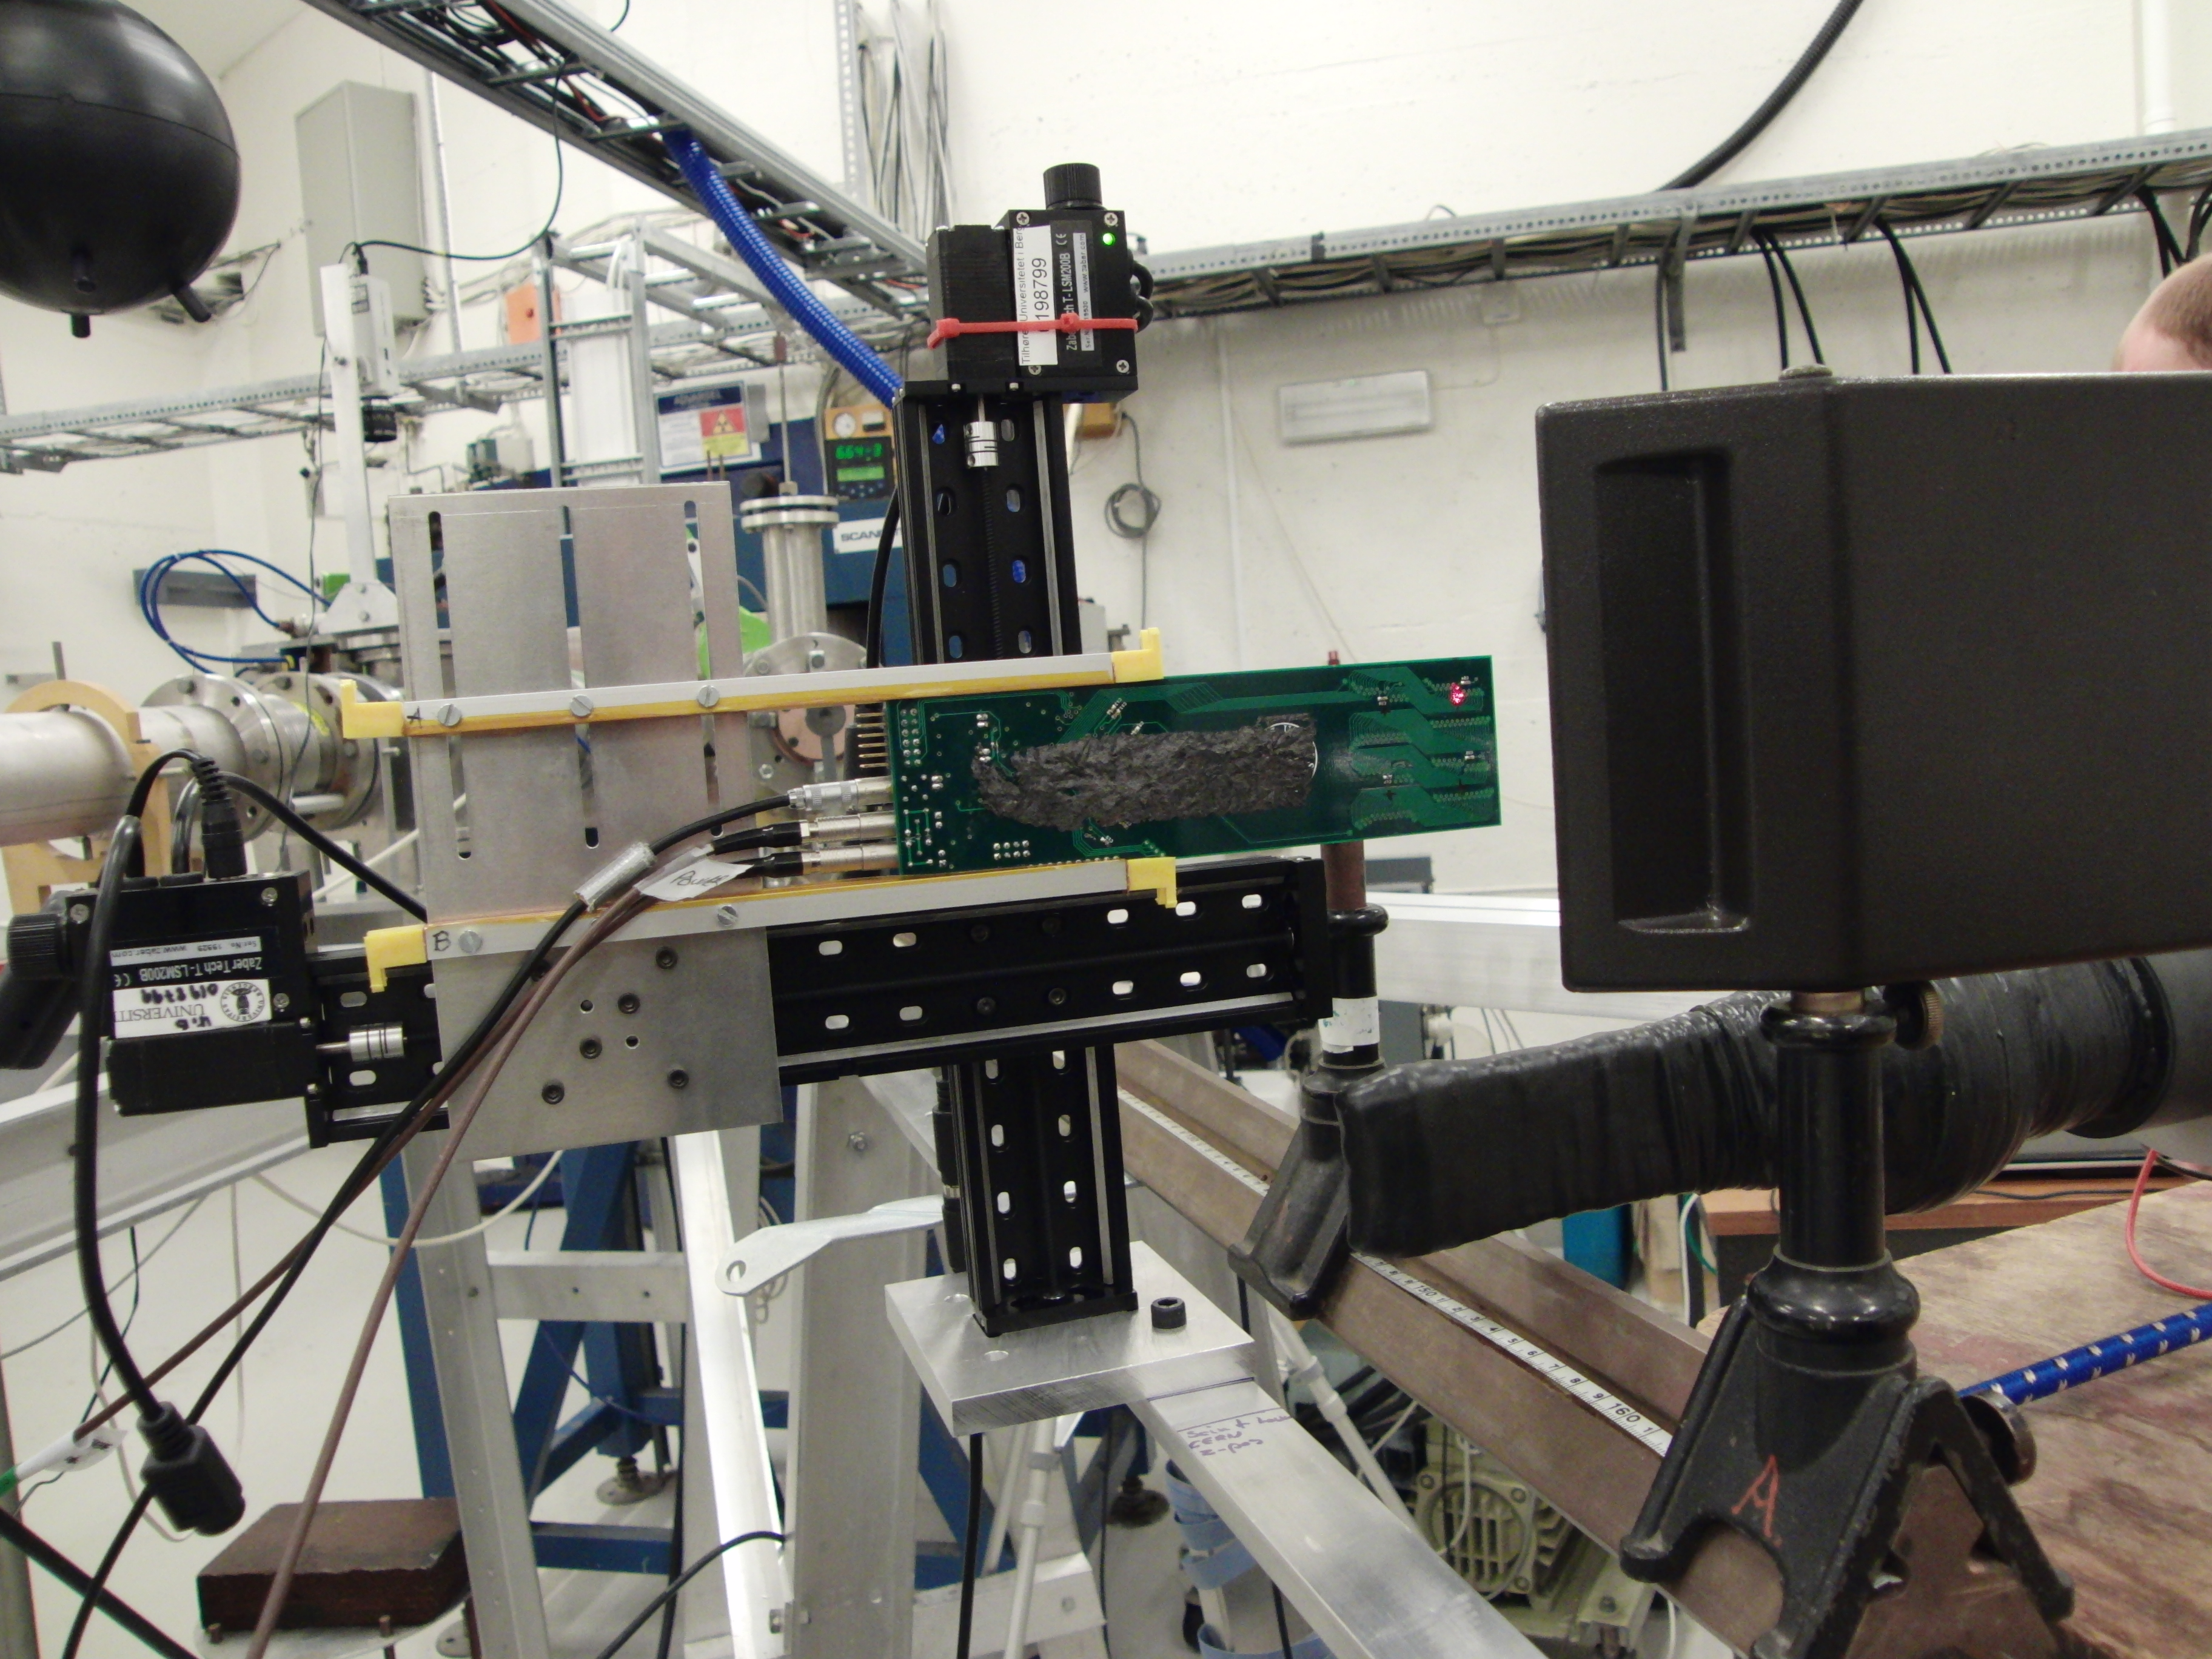
\includegraphics[width=\linewidth]{figures/XY_back}
  \caption{X-Y-positioning system upfront}
  \end{subfigure}
 \caption[X-Y-Positioning System]{X-Y-positioning system upfront and behind stationed in OCL. The SRAM radiation detector is mounted}
 \label{xy-table}
\end{figure}
\newpage


\chapter{Irradiation Test Setup}
Irradiation tests for the RCU2 electronics  were executed at two facilities: \acf{OCL} and \acf{TSL}.
This chapter will give a brief introduction to the two facilities, and explain the preparation process for each of the two them.

The purpose of testing the RCU2 electronics for radiation is to see if the tested components are able to survive in a radiation hard environment as we will find in the \ac{TPC}, see section \ref{how_to_test}.
To test the limit for each of the components, the components was irradiated until an error was detected, current consumption drastically increased or the components received a much higher dose than were required without any error.

\section{Irradiation on \ac{OCL}}
Oslo Cyclotron Laboratory is located at the Department of physics at the University of Oslo, and was opened in 1978. The cyclotron is of the type MC-35 and was made by Scanditronix AB from Sweden.
This is the only accelerator in Norway for ionized particles used in basic research.
The cyclotron can accelerate protons, deuteron, $^3He$ and $^4He$, 
with energies and intensities as seen in the table \ref{design requirements} below.
A drawing of the lab can be seen in figure \ref{OCL_fig}. 
The laboratory is divided in three; the control room, the inner experimental hall and the outer experimental hall.
The cyclotron is placed in the inner hall, and a beam is sent through pipes to the outer hall.
Inside the cyclotron and the pipes there is vacuum, so that the particle should not suffer energy loss from collision with air molecules.
With magnets it is possible to regulate the beam to your desired pipe exit.
There are also several cups put on the pipeline which makes it possible to block the beam.
These can be used to stop the beam during an experiment, so that it is possible to go into the experimental area and do changes on your setup.
When the cyclotron is running and the beam is on, you are not allowed to enter the inner experimental area.
 
\begin{figure}[!htbp]
\centering
\centerline{\includegraphics[height=7cm,width=8cm]{figures/OCL}}
\caption{Layout of the beam area at OCL}
\label{OCL_fig}
\end{figure}


\begin{table}[!htbp]
 \centering
\begin{tabular}{|l|l|l|}\hline
Ionized beam particle type & Energy(${\mega\electronvolt}$) & Intensity($\micro\ampere$)  \\ \hline \hline
Proton & 2-35 & 100 \\ \hline
Deuteron & 4-18 & 100 \\ \hline
$^3He$ &  6-47 & 50 \\ \hline 
$^4He$  & 8-35 & 50 \\ \hline
\end{tabular}
\caption{Ionized beam particle data table}
\label{design requirements}
\end{table}

\subsection{Experiment Setup and Equipment}

The experiment setup was placed in the outer experimental hall in experimental area 2. The experimental setup as well as the equipment used can be found in the figure and table below.
The equipment was kept in a height of 140-150cm. Beam exit was in a height of 141.5cm.
  
\begin{figure}[!htbp]
\centering
  \centerline{\includegraphics[width=0.5\textwidth]{figures/experiment_setup}}
  \caption{Experimental setup seen from above}
  \label{experiment_setup}
\end{figure}%
  
\begin{figure}[!htbp]
  \centering
  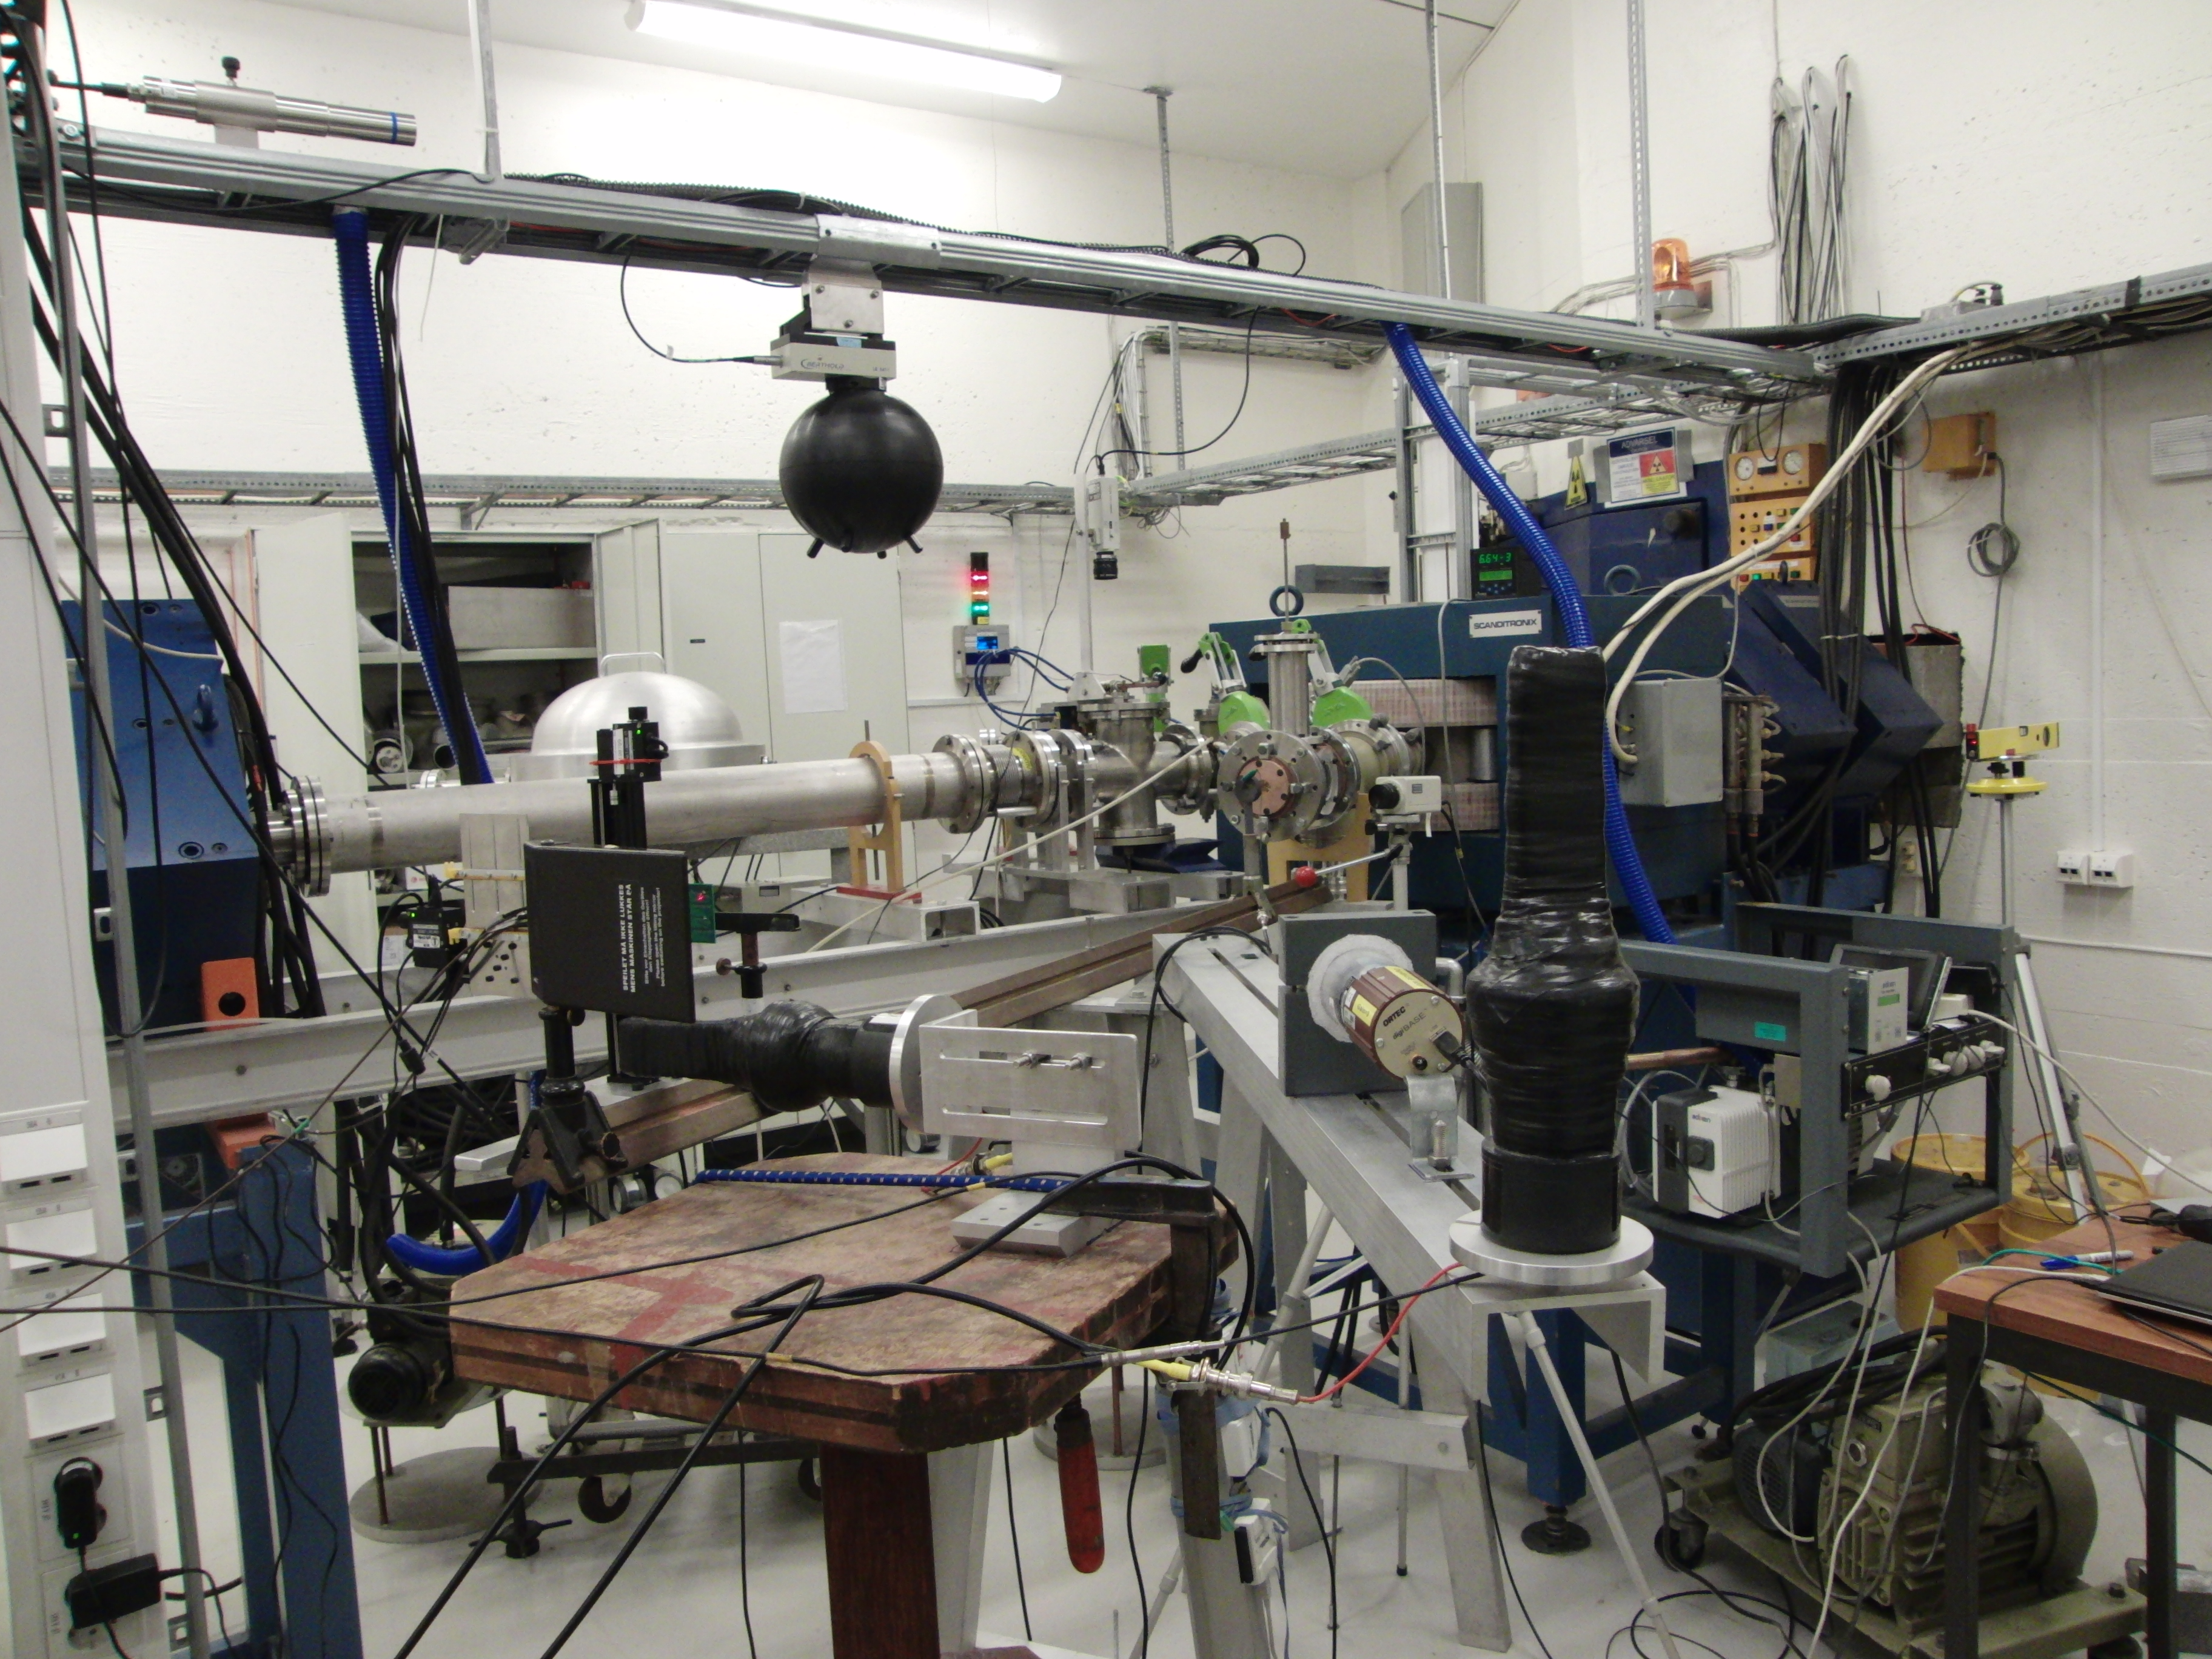
\includegraphics[width=\textwidth]{figures/experiment_area}
  \caption{Picture of the experimental area}
  \label{experiment_area}
\end{figure}


\newpage
\begin{table}[!htbp]
 \centering
\begin{tabular}{|l|p{10cm}|}\hline
Equipment & Explanation  \\ \hline \hline
Scintillator & A plastic scintillator with photomultiplier. Was used to measure relative radiation. We had two of these, one that was placed directly under \acf{DUT} and one that was placed 75cm away from \ac{DUT}. \\ \hline
High voltage regulator & Voltage for the photomultiplier. 800V was used. \\ \hline
The test boards &  TPS51200, MIC69302WU, SN74AVCB164245, SN74AVC2T245, QS3VH257, SY89831U, ADN2814, MAX3748, INA210, TLV3011 and SF2 starter-kit. \\ \hline 
SRAM radiation detector  & A PCB board with 4 \ac{SRAM} cells that was used to characterize the beam and to measure scintillator counts \\ \hline
SF2 starter kit & A starter kit board with the \acf{SF2} \ac{SoC} \ac{FPGA}.  \\ \hline
Computer  & A VNC server was set up on a computer inside the experimental hall, which made it possible to control the experiment from the control room. The computer was running all the necessary software to control and monitor the experiment. \\ \hline
USB DAQ  & Data acquisition board form National Instruments (NI). Used to establish analog and digital connection to the test boards and send data to the computer. \\ \hline
Radiation film  & A film of the type \emph{grafchromic} that reacts when irradiated. Used to identify the beam. \\ \hline
leveled laser  & Was used to pinpoint the center of the beam.\\ \hline
Mirror & Used to reflect the laser beam to the backside of the test boards.\\ \hline
XY-positioning system  & Connected to the computer so that we could change the position of the test boards from a computer \\ \hline
\end{tabular}
\caption{Equipment used in the experiment}
\label{equipment}
\end{table}

\subsection{Preparation and characterization of the beam}
\label{beam_setup}
The first thing to do before we could start our radiation test is to characterize the beam, to see that it hit around the area that we expected.
This was done by using radiation films that turns black when exposed to radiation. 
One of these was placed directly in front of the beam exit and one in front of \acf{DUT} area. This was done to see how the beam spread out, and to get a indication of where the beam center was.
Afterwards a more precise calibration was performed by the use of the SRAM radiation detector and the scintillator. 
By measuring the relation between scintillator counts on the scintillator which was in a locked position and SEU on the \ac{SRAM} that was connected to the XY-position system (which made the \ac{SRAM} freely to move), we were able to find a more precise position of the beam center by observing which position gave us the highest number of SEUs compared to scintillator counts.
When the beam center was found and everything worked as it should, the laser was placed in a position so that the laser beam pointed to where we had found center of the beam to be. Thereafter we could replace the \ac{SRAM} board with the PCB that we were going to test. This had to be done every day at startup, before we could start the actual tests.

We were able to control the intensity (Current) of the beam freely from the control room inside the limitation of the beam (for protons that is up to 100 $\micro\ampere$), but we kept us in the area between 100 $\pico\ampere$ to a few $\nano\ampere$. This way the radiation dose to the test boards could be controlled. The beam intensity could be measured by putting a Faraday Cup (FC)in front of the beam, which was connected to a high accuracy multimeter. The FC had to be removed when tests were running, since it would block the beam.

We were running up to 3 LabVIEW programs through the experiment, one for controlling the XY-position system,
one for the \ac{SRAM} board (to measure SEU and scintillator counts when calibrating and to get scintillator counts during the tests) and one program for each of the test boards.
The \ac{SRAM} and test board programs were constantly saving data on the disk.

\subsection{What was Tested at OCL}
We had beam time in three periods at OCL; $13.11.13-15.11.13$, $28.11.13-29.11.13$ and $08.04.14-11.04.14$. What were tested in the respectively periods, can be seen in \autoref{test_ocl}.
% The boards that were tested in the first period are: $TPS51200_1$, $MIC69302WU_1$, $SN74AVCB164245_1$, $SN74AVC2T245_1$, $QS3VH257_1$ and $SY89831U_1$, tested in that order.
% In the second period we tested: $ADN2814$, $MAX3748$, $SY89831U_2$, $TPS51200_2$, $MIC69302WU_2$, $SN74AVCB164245_2$, $SN74AVC2T245_2$ and $QS3VH257_2$, in that order.
% And in the third period, the focus was mainly on the \ac{SF2} starter-kit, but $INA210_1$, $INA210_2$, $TLV3011_1$ and $TLV3011_2$ were also tested.
\begin{table}
 \centering
 \begin{tabular}{|l|p{10cm}|} \hline
 Test period & Tested boards \\ \hline \hline
 $13.11.13-15.11.13$ & $TPS51200_1$, $MIC69302WU_1$, $SN74AVCB164245_1$, $SN74AVC2T245_1$, $QS3VH257_1$ and $SY89831U_1$ \\ \hline
 $28.11.13-29.11.13$ & $ADN2814$, $MAX3748$, $SY89831U_2$, $TPS51200_2$, $MIC69302WU_2$, $SN74AVCB164245_2$, $SN74AVC2T245_2$ and $QS3VH257_2$ \\ \hline
 $08.04.14-11.04.14$ & $INA210_1$, $INA210_2$, $TLV3011_1$, $TLV3011_2$ and SF2 M2S050ES-T-FG896\\ \hline
 \end{tabular}
 \caption{Overview of the tested components at OCL}
 \label{test_ocl}
\end{table}

\newpage

\section{Irradiation at \acf{TSL}}|
The main difference between \ac{OCL} and TSL is that TSL is able to produce a beam of much higher energies. TSL is a much more professional facility, meaning that there are more people working there available for assistance, and there is no need for any calibration before starting a radiation test. We can simply show up and expose what we want to expose, and data, like fluence and exposed time, are given to use, making it easy for us to calculate the dose and flux. 

TSL is an accelerator facility belonging to University of Uppsala in Sweden, \cite{website:TSL}.
It is mainly used for proton therapy on cancer patients by Uppsala University Hospital, but it is also used for medical research and radiation testing of electronics. The heart of the installation is a Gustav Werner cyclotron that delivers a beam of charged particles in energies up to 192 MeV. The particles that can be produced are everything from protons to highly charged xenon ions.
There are several extraction points from the cyclotron, which are controlled from the \emph{control room}. The beam can be lead out into the \emph{blue hall}, which is the experiment area used for electronics testing. The Blue hall has two user areas; one for protons, and one for neutrons and heavier ions, see \autoref{Blue_hall}.

\begin{figure}[!htbp]
  \centering
  \includegraphics[width=0.7\textwidth, angle =-2.5]{figures/Blue_hall}
  \caption{Layout of the Blue hall}
  \label{Blue_hall}
\end{figure}

\subsection{Beam Setup Procedure}
At TSL we didn't have to get a beam characterization as we did at \ac{OCL}. In the Blue hall there is a permanently setup with detectors and a well-defined beam line. We only needed to set up our test equipment, put the test board at a given extraction point, and start the test. The center of the beam was found by lasers placed in locked positions around the hall, one for horizontal direction and one for vertical direction. The head of the laser was movable, so we could point the laser beams towards our test board. A computer which was remotely controlled through network connection was placed in the hall.
This computer was used as a connection point to our test boards. We sat in a room called \emph{counting room}, where we could turn the beam on and off as we desired. There was also a machine in the counting room that was connected to detectors in the blue hall, telling us the fluence (number of protons per $\centi\meter^2$ in total) and exposed time. The fluence can be used to calculate the flux and dose. The energy of the proton beam we got was 170 MeV.

\begin{figure}[!htbp]
  \centering
  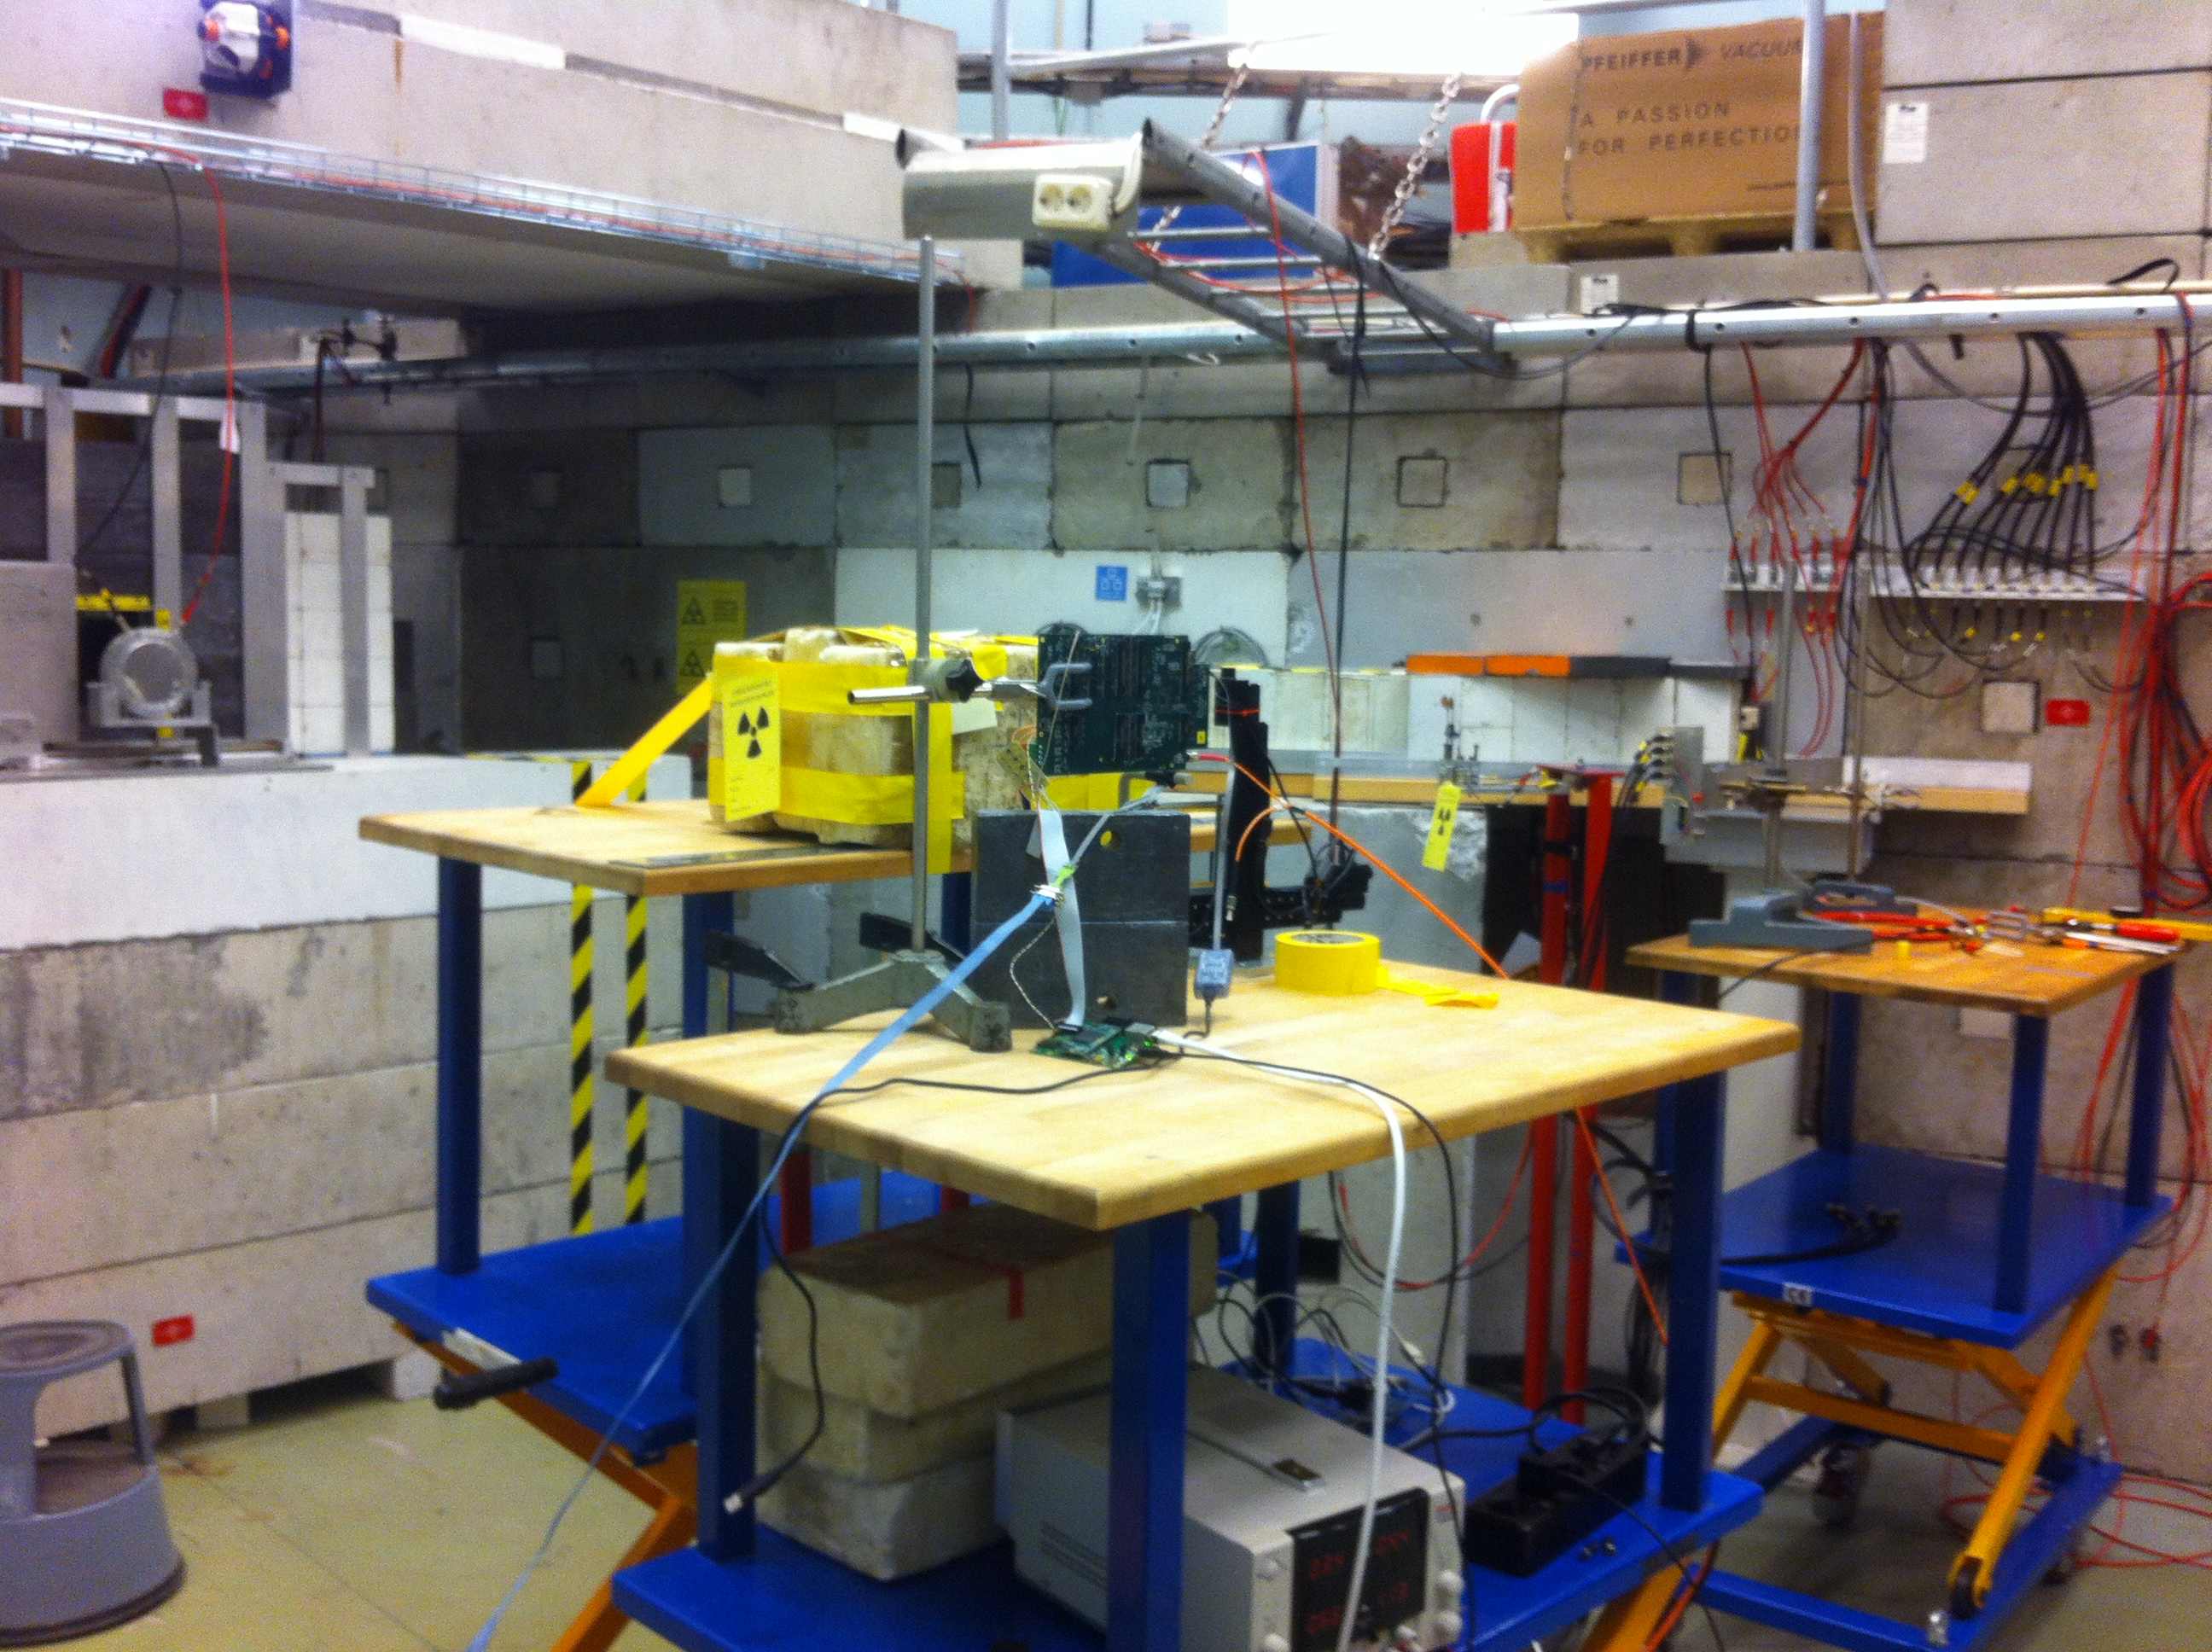
\includegraphics[width=0.7\textwidth]{figures/TSL_setup}
  \caption{Setup in the blue hall. The RCU2 is mounted, ready to be exposed for radiation}
  \label{TSL_setup}
\end{figure}

\subsection{What were Tested at \ac{TSL}}
A week before we arrived at TSL, we got the first two prototypes of the RCU2. That means that we had limited time to make tests for all of the different parts of the board. 

The focus of the visit to TSL was the SF2 SoC FPGA, but we also tested an optical receiver and an optical data link, which respectively are being used for TTC (timing, trigger and control) and to send data from the RCU2.
We brought with us two RCU2s and a total of 7 starter-kits, where 3 of these had a smaller package of SF2, M2S050-FG484, and the rest were engineering samples versions of M2S050-FG896, which is the one used on RCU2.
For the tests as discussed in \autoref{SF2_section}, we only used the SF2 starter-kits, since the test only involves internal parts of the SF2 SoC FPGA. Two of the starter-kits with the smaller package (M2S050-FG484) were tested, and one with engineering sample (M2S050ES-T-FG896). When the RCU2 cards were exposed to radiation, things like detector data link (DDL), trigger, clock and data recovery (CDR) and PLL were tested, which will not be discussed thoroughly in this work, but a short summary will be given. Current was measured on the SF2 starter-kits and the RCU2 boards when they were irradiated to check for latchup.


\chapter{Calculations and Results from Radiation Tests}
\emph{This chapter will explain how the collected data from radiation tests were used to calculate flux and dose, and results from radiation tests at \ac{OCL} and \ac{TSL} will be presented and discussed.}

After an irradiation test at \ac{OCL}, the collected data consists of the exposed time, scintillator counts, current consumption and output data of the \ac{DUT}.
From the calibration before radiation test, we found the relation between scintillator counts and \ac{SEU} on the SRAM radiation detector. From earlier tests with the SRAM radiation detector the cross section for an incoming proton to induce a \ac{SEU} is known. These data are used to calculate the received dose for each components. The next section will explain the calculation process.

% \ac{TSL} is a facility which sells beam time for a living. So all data after a radiation was given to us, and we didn't need to do any beam monitoring ourself. We only needed to mount the test board that we wanted to test in test spot, and all data like fluence and dose where received from the facility. At \ac{OCL} however, we had to do the hole monitor process and calculate everything ourself, and required therefore much more time before and after radiation. The next sections will explain the calculation process after radiation at \ac{OCL}.

\section{Calculation of Dose}
Two ways to calculate the dose will be discussed in this section; manually using energy loss and \ac{LET}, see section \ref{radiation_phys}, and simulation data from a program named FLUKA. Which of these gives us the most reliable result will be discussed at the end of this section.

\subsection{Definitions}
\label{difinitions}
Absorbed radiation dose has the unit of energy/mass and the SI-unit is gray (Gy), which is 1 Joule of energy absorbed in a kilogram of matter [J/Kg], see equation \ref{Joule_kg}.
Another unit often used when it comes to radiation of electronics is Rad, short for "Radiation absorbed dose".
The relation between Rad and Gy can be seen in equation \ref{Gy_to_Rad}.

\begin{equation}
1 Gy = 1 \frac{\joule}{\kilogram}
\label{Joule_kg}
\end{equation}

\begin{equation}
1 Rad = 0.01 Gy = 0.01 \frac{\joule}{\kilogram} = 10^{-5} \frac{\joule}{\gram}
\label{Gy_to_Rad}
\end{equation}

The particle energy is normally expressed in electronvolt ($\electronvolt$) or Megaelectronvolt ($\mega\electronvolt$). One electronvolt is defined as the amount of kinetic energy gained by a single unbound electron when it accelerates through an electric potential of one Volt, thereof $\electronvolt$. Its value is $e = 1.602 \times 10^{-19} C$ which is the electric charge, multiplied with one Volt, which equals $1.602 \times 10^{-19}\electronvolt$ or $1.602 \times 10^{-19}\joule$.

\begin{equation}
1 \mega\electronvolt = 10^{6} \electronvolt = 10^{6} \cdot 1.602 \times 10^{-19}\joule = 1.602 \times 10^{-13}\joule
\label{MeV_to_joule}
\end{equation}

\subsection{Calculating Dose Using LET}
\label{using_LET}
% When using \ac{LET} to calculate the dose, we are looking at the total energy that is deposited in a component.
As explained in \autoref{LET_section}, \ac{LET} is energy deposited in a material through ionization when a particle crosses the material.
% To calculate this energy, we need to know the thickness, density and area of the material, which particle that enters the material and its energy.
\ac{LET} is equal to the energy loss a particle suffer by crossing a material, which means that we can use the Bethe Bloch formula that is expressed in equation \ref{stopping_power}.
By looking at total \ac{LET} for an component while knowing the fluence, the dose can be  calculated, see \autoref{Dose_rad}.
The energy loss of a particle is highly energy dependent, but for short distances it can be assumed to be constant without getting any noticeable error.

Two energies were used when exposing components at \ac{OCL}. The first time a proton beam with an energy of 28 MeV, and the two other times a beam of 25 MeV.
\ac{DUT} was placed 130 cm away from beam exit, which means that the protons would suffer some energy loss in the air between beam-exit and \ac{DUT}. To make the work easier for us, an energy loss calculator program \cite{website:energyloss_calculator} was used to calculate the \emph{energy loss} for a 28 $\mega\electronvolt$ and a 25 $\mega\electronvolt$ proton beam in air, we got respectively $17.52 \frac{\mega\electronvolt\centi\meter^2}{\gram}$ and $19.2 \frac{\mega\electronvolt\centi\meter^2}{\gram}$.
By multiplying with the density of air which is $\rho_{air}=1.275\frac{\milli\gram}{\centi\meter^3}$, we got $22.3 \frac{\kilo\electronvolt}{\centi\meter}$ and $24.5 \frac{\kilo\electronvolt}{\centi\meter}$. This means that the energy of the protons when they collide into \ac{DUT} is:

\begin{equation}
E_{proton1} = 28 - (130 \centi\meter \times 22.3 \frac{\kilo\electronvolt}{\centi\meter}) \approx 25 \mega\electronvolt
\label{Proton_energy1}
\end{equation}

\begin{equation}
E_{proton2} = 25 - (130 \centi\meter \times 24.5 \frac{\kilo\electronvolt}{\centi\meter}) \approx 22 \mega\electronvolt
\label{Proton_energy2&3}
\end{equation}

By using the same energy loss calculator we find find that the energy loss in silicon (which is the main component in integrated circuit), to be:

\begin{equation}
-\frac{dE}{dx} (25 MeV) =  17.1 \frac{\mega\electronvolt\centi\meter^2}{\gram}
\label{energy_loss_25}
\end{equation}

\begin{equation}
-\frac{dE}{dx} (22 MeV) =  18.9 \frac{\mega\electronvolt\centi\meter^2}{\gram}
\label{energy_loss_22}
\end{equation}

Looking into a single proton entering a silicon material, the energy deposited by that single proton can be expressed as;

\begin{equation}
\Delta E_{proton} = -\frac{dE}{dx} \cdot \Delta x \cdot \rho_{Si}
\label{proton_energy_loss}
\end{equation}

where $\Delta x$ is the length segment a proton particle penetrates into the material, and $\rho_{Si}$ is the density of silicon.

\begin{equation}
\rho_{Si} = 2.33 \frac{\gram}{\centi\meter^3}
\label{silicon_density}
\end{equation}

To determine the total energy deposited in the component, we have to multiply the energy of a single proton with the fluence and the area of the component. Fluence is the total flux over a given time, expressed in [$\frac{n}{cm^2}$], where n is number of protons. The total energy is then:

% Flux = \Phi
\begin{equation}
\Delta E_{total} = \Delta E_{proton} \cdot fluence \cdot A_{Si} = -\frac{dE}{dx} \cdot \Delta x \cdot \rho_{Si} \cdot fluence \cdot A_{Si}
\label{total_energy_loss}
\end{equation}

Now we know the total energy depleted by a proton beam in an component, and can start calculating the dose. Dose is energy per mass, as explained in section \ref{difinitions}. Meaning that the absorbed dose in silicon can be expressed as,

\begin{equation}
Dose(Si) = \frac{-\frac{dE}{dx} \cdot \Delta x \cdot \rho_{Si} \cdot \Phi \cdot A_{Si}}{m_{Si}}
\label{Dose(si)}
\end{equation}

where $m_{Si}$ is the mass of silicon.

$m_{Si}$ can be expressed in terms of silicon density, see equation \ref{silicon_density}, multiplied with the volume ($V_{Si}$), which is Area ($A_{Si}$) times thickness ($d_{Si}$). Assuming that the protons enter the silicon in a straight line, the path segment $\Delta x$ is equal the thickness, which then gives us:

\begin{equation}
Dose(Si) = \frac{ -\frac{dE}{dx} \cdot \Delta x \cdot \rho_{Si} \cdot \Phi \cdot A_{Si}}{\rho_{Si} \cdot A_{Si} \cdot d_{Si}} = -\frac{dE}{dx} \cdot fluence = [\frac{MeV}{g}]
\label{Dose_silicon}
\end{equation}

To determine the dose in Rad instead of $\frac{MeV}{g}$, we multiply with the converting factor given in equation \ref{MeV_to_joule} and divide by the factor given in equation \ref{Gy_to_Rad}. This gives us:

\begin{equation}
Dose(Si) = 1.602 \cdot 10^{-8} \cdot -\frac{dE}{dx} \cdot fluence
\label{Dose_rad}
\end{equation}

\subsection{Calculating Dose Using FLUKA Simulations}
The FLUKA Monte Carlo code is a well benchmarked general purpose tool for calculations of particle transport and interactions with matter, covering an extended range of applications like for example proton and electron accelerator shielding, target design, calorimetry, activation and dosimetry, cosmic ray studies, and radiotherapy. It can simulate with high accuracy the interaction and propagation in matter of about 60 different particles, including photons and electrons from 1 keV to thousands of TeV, neutrinos, muons of any energy, and hadrons of energies up to 20 TeV \cite{website:FLUKA}.

We simulated a proton beam with energy of 28 MeV and 25 MeV in air, and set our \ac{DUT}-position 130 $\centi\meter$ away from beam exit. The results can be seen in table \ref{FLUKA_simulations}.

% Table generated by Excel2LaTeX from sheet 'FLUKA'
\begin{table}[!htbp]
  \centering
    \begin{tabular}{|l|l|l|} \hline
    Energy at beam exit & 28 MeV & 25 MeV  \\\hline\hline
    Dose/primary particle at DUT[Gy] & 4.08E-10 & 2.94E-10 \\\hline
    Primary particles at Beam exit & 1 & 1 \\\hline
    Primary particles at DUT & 0.1331 & 0.0857 \\\hline
    Beam intensity reduction at DUT & 7.51 & 11.67\\\hline
    \end{tabular}%
      \caption{FLUKA simulation with 28MeV proton beam}
  \label{FLUKA_simulations}%
\end{table}%

As mentioned in the introduction to this chapter, the known values after a radiation test are exposed time, scintillator counts, current consumption, output data of the \ac{DUT} and cross section from the SRAM radiation detector.

The procedure to calculate the dose starts with finding the total fluence. This is found by first converting from scintillator counts to SEU, by multiplying with the converting factor as found in the beam setup. And then divide on the cross section, which is known for the SRAM radiation detectorm, see \autoref{SRAM_section}. Fluence can then be found as seen in equation \ref{FluenceDUT} and the flux as in equation \ref{flux}.

\begin{equation}
FluenceDUT = \frac{SEU}{CS}
\label{FluenceDUT}
\end{equation}

\begin{equation}
Flux = \frac{Fluence}{time}
\label{flux}
\end{equation}

The FLUKA simulation results tells us how many protons will collide into \ac{DUT} for each proton coming out from beam exit, and what dose this will contribute to at \ac{DUT}. By using the calculated Fluence for DUT, found by equation \ref{FluenceDUT}, we can find the fluence at beam exit by dividing on \emph{primary particles at \ac{DUT}} from the simulation results, see equation \ref{FluenceBE}.
Then we can use \emph{dose per primary particle at DUT} from the result and multiply with the Fluence at beam exit, which gives us the dose in gray for the \ac{DUT}, see equation \ref{DoseDUT}. By multiplying by 100 we get the dose in Rad.

\begin{equation}
FluenceBE = \frac{fluenceDUT}{primaryparticlesDUT}
\label{FluenceBE}
\end{equation}

\begin{equation}
DoseDUT = FluenceBE \cdot \frac{Dose}{primaryparticleDUT} = [Gy]
\label{DoseDUT}
\end{equation}

\subsection{Comparison of LET and FLUKA calculations}
The results from radiation of MAX3748 can be used to compare LET calculation with FLUKA, the test results can be found in \autoref{MAX3748_results}.
Both methods to calculate dose require the fluence. The fluence is given by SEU on SRAM, and cross section, see \autoref{FluenceDUT}, and SEU on SRAM are given by the conversion factor found in beam setup and scintillator counts. For MAX3748 the fluence is:

\begin{equation}
Fluence_{MAX3748} = \frac{2698510 \cdot 0.473}{1.14\cdot10^{-6}} = 1.12\cdot10^{12}\frac{n}{\centi\meter^2}
\label{FluenceMAX3748}
\end{equation}

\begin{table}[!htbp]
  \centering
  \begin{tabular}{|l|l|} \hline
  time 				& 2472 s \\\hline
  proton energy Beam exit  		& 25 MeV \\\hline
  scintillator counts 		& 2698510 \\\hline
  scintillator counts to SEU SRAM 	& 0.473 \\\hline   
  Cross section 			& $1.14E-6 \frac{cm^2}{device}$\\\hline
  \end{tabular}
  \caption{Results after radiation of MAX3748}
  \label{MAX3748_results}
\end{table}

To calculate the dose using LET, we follow the steps given in \autoref{using_LET}.
Starting by calculating the energy when entering the component 130 cm away from beam exit. This is found in equation \ref{Proton_energy1} to be 22 $\mega\electronvolt$.
LET, or energy loss, for a 22 $\mega\electronvolt$ proton particle in silicon, is calculated in equation \ref{Proton_energy2&3} to be 17.1 $\mega\electronvolt$.

Fluence is found in equation \ref{FluenceMAX3748}. By using \autoref{Dose_rad} we find the total dose in Rad to be:

\begin{equation}
Dose(Si)= 1.602 \cdot 10^{-8} \cdot 17.1 \cdot 1.12\cdot10^{12} = 306.8 kRad
\label{Dose_rad_MAX3748}
\end{equation}

Calculation using FLUKA simulation is an easy process, starting by calculating the fluence at Beam exit, from equation \ref{FluenceBE}, and then using that value to calculate the dose as seen in  \autoref{DoseDUT}.

\begin{equation}
FluenceBE = \frac{1.29\cdot10^{12}}{0.0857} = 1.51\cdot10^{13}\frac{n}{\centi\meter^2}
\label{FluenceBE_MAX}
\end{equation}

\begin{equation}
DoseDUT = 1.51\cdot10^{13} \cdot 2.94\cdot10^{-10} = 4425.4 Gy = 383.8 kRad
\label{DoseMAX3748}
\end{equation}

We can see that the FLUKA results give approximately 20 \% higher dose than by using LET. Why we have this difference will be discussed.

When calculating LET for a given component we calculated with constant energy drop through the air before colliding with the component and through the component. In reality energy loss will increase as the energy decreases. This means that the calculated dose is a little lower than the actual dose.

% FLUKA simulation are being used for advance simulations for people at CERN and all over the world, and is an acknowledged program.
% It is based on Monte Carlo simulations, and several models are used for the calculations, for example Bethe Bloch theory, Beth $Z^2$, Barkas $Z^3$ and a lot more \cite{website:FLUKA}. Having many models tested up against each other, tells us that the calculated values are quite reliable.

When using LET to calculate the dose, we get a small error from approximations and assumptions. But since we know about these, we also know that the energy should be a little higher than the calculated value, and can be sure that the calculated dose is at least not higher than the actual dose.
The FLUKA simulations are using advance models for the calculations, which makes the results very accurate.

Other than the calculation method, there may also be other sources of errors, like that the energy level of the proton beam (it may differ from 28/25 MeV which it is said to be), the conversion factor found in the beam setup and unlinearity between scintillator counts and SEU on SRAM. Which means that if the calculation method is precise, we will still get errors due to other error sources. We are nevertheless manly interested in getting a total dose which is more than the total dose it will receive in the ALICE TPC, and the accuracy isn't that important as long as it is over this level with a safety margin.
% And when we have other factors which may not be as accurate, the dose calculations doesn't need to be hundred present accurate.
% For our calculated data we are mostly interested in the dose level, and doesn't care so much about the accuracy, as long as it is in a reasonable range.
That means that both of the methods are good enough.

At OCL, FLUKA simulation was used to calculate the dose, and at TSL, LET was used to calculate the dose.

\section{Results from OCL}
\subsection{Calibration process}
As explained in chapter $\ref{beam_setup}$, we had to start by finding the center of the beam.
The laser was first placed in a position pointing at what was thought to be center. 
Then we placed a radiation film in front of the beam exit and at \ac{DUT} area.
By observing how the radiation films were after irradiation, we got a indication of where the center of the beam was.
An example of two films from the beam exit and \ac{DUT} area can be seen in figure \ref{Radiation_film}.

\begin{figure}[!htbp]
  \centering
  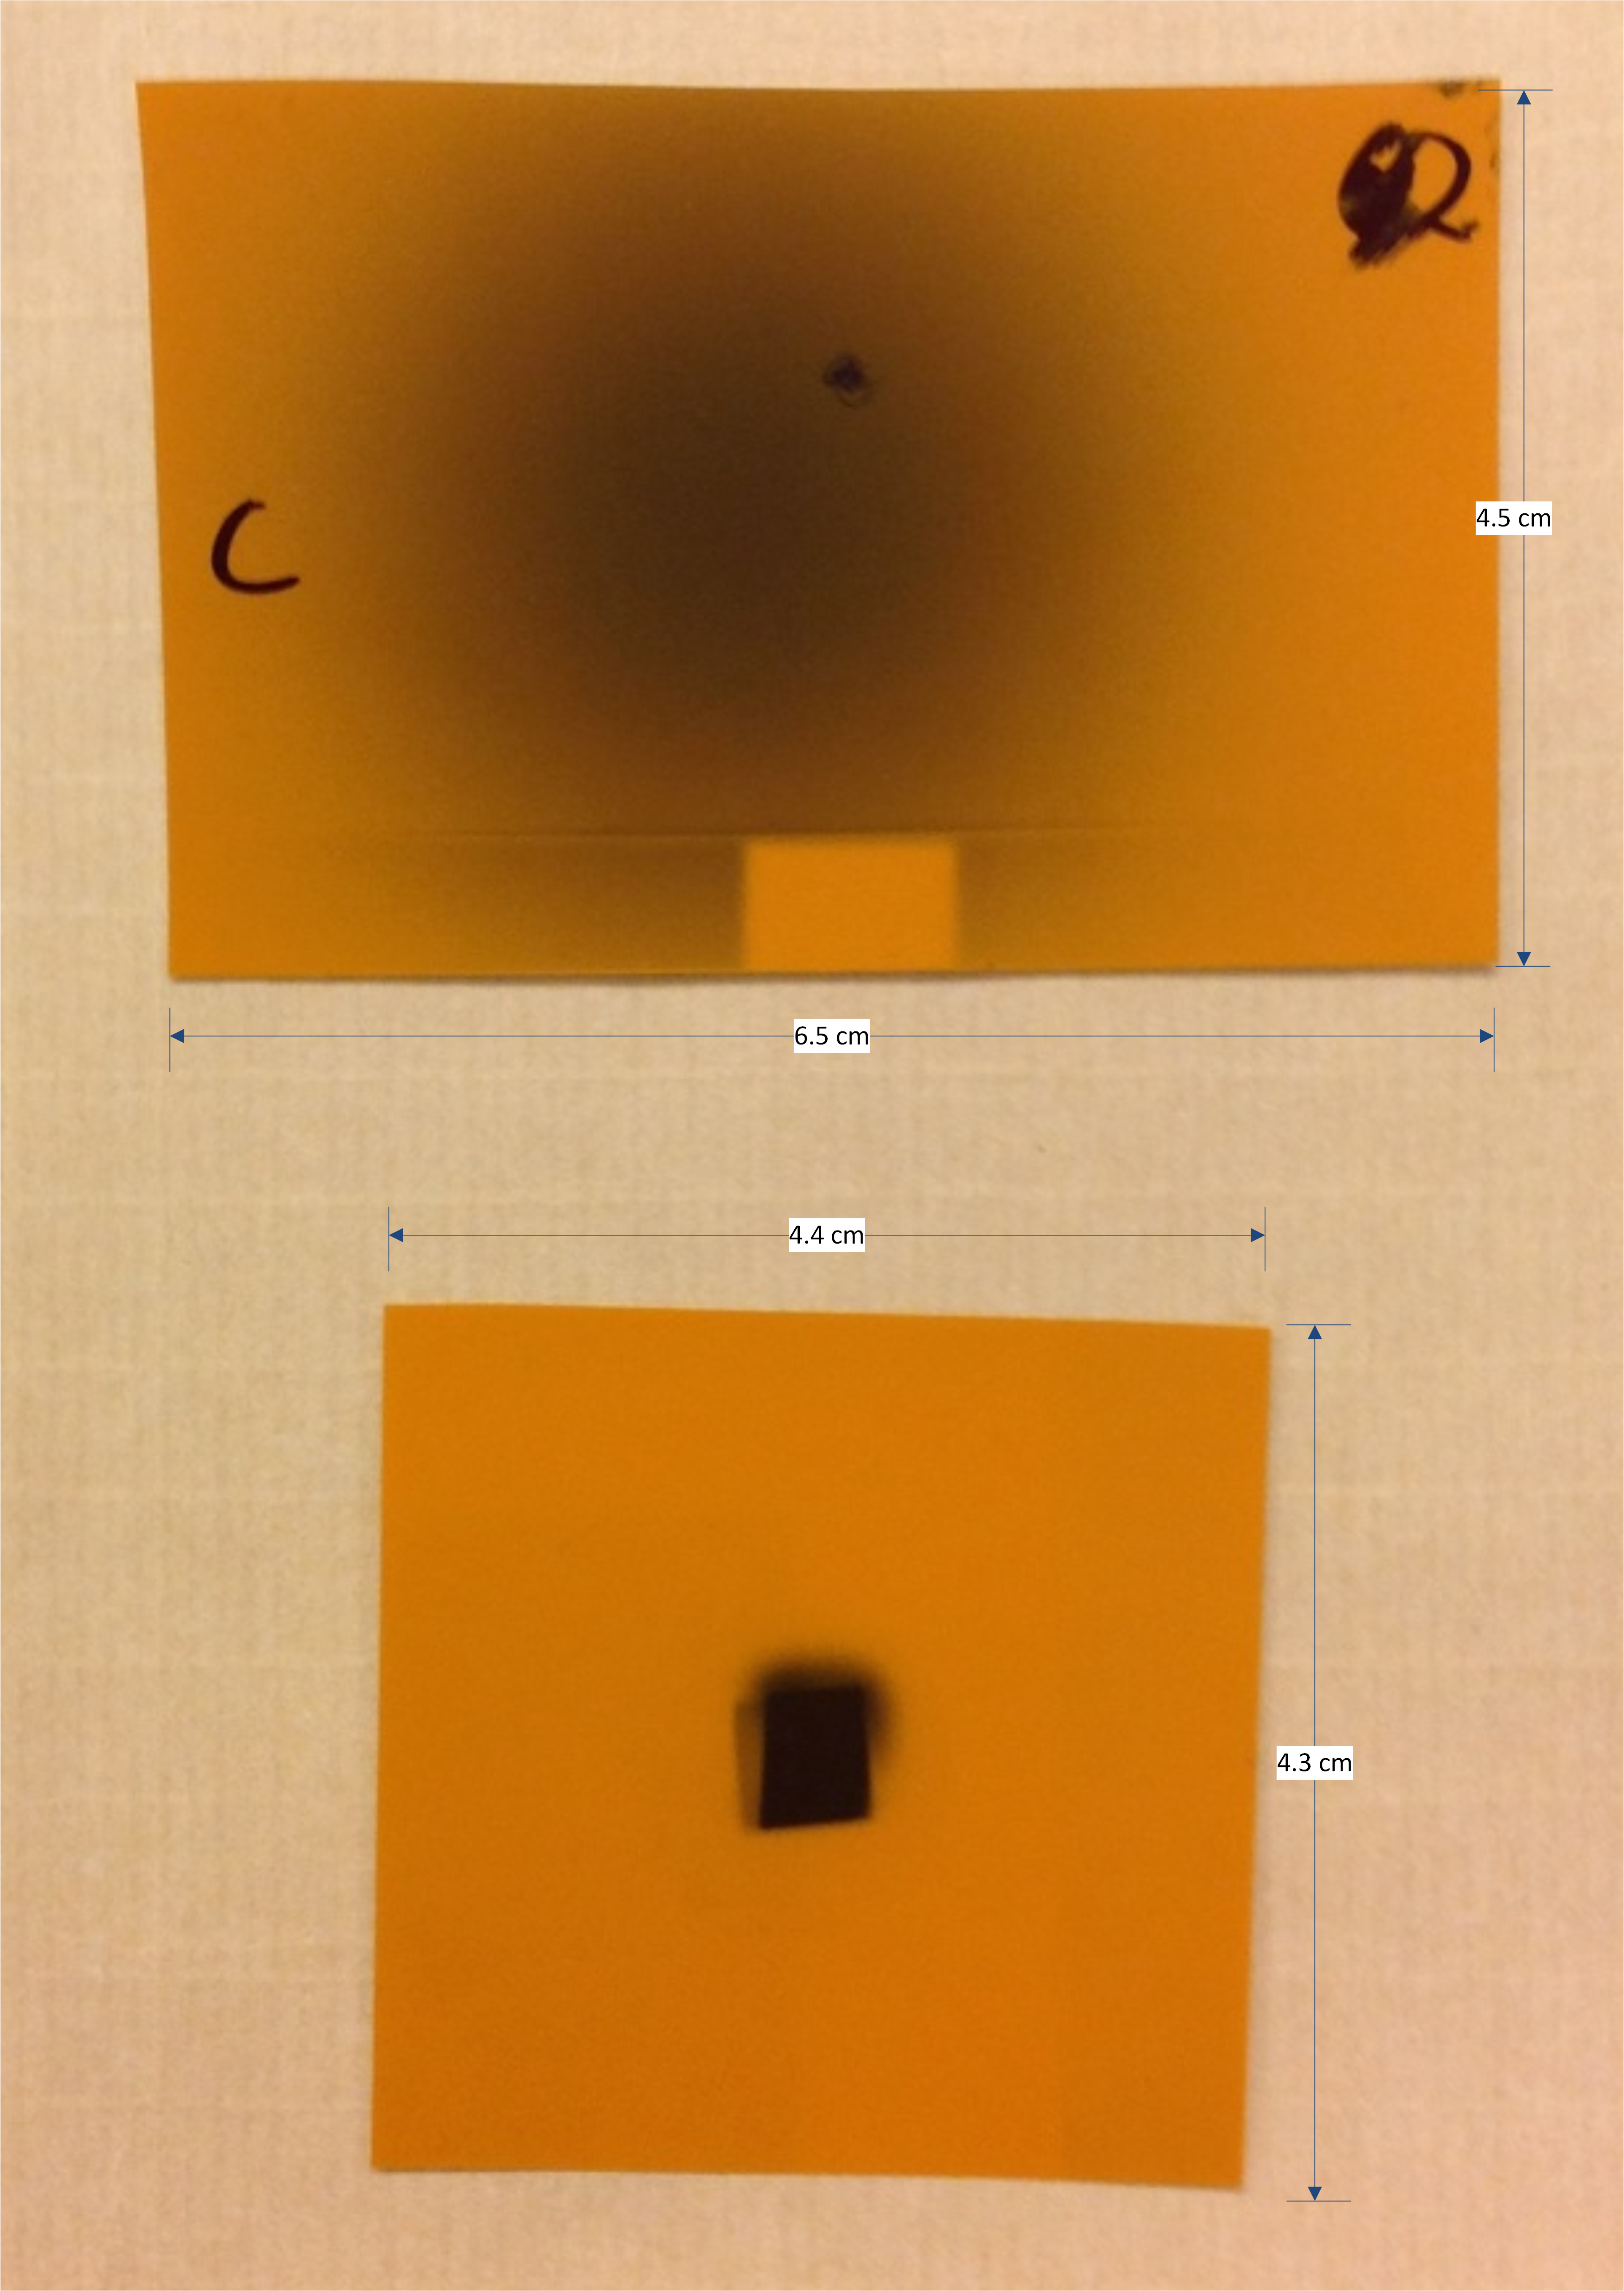
\includegraphics[width=0.5\textwidth]{figures/radiation_film2}
  \caption[Radiation Film]{Example of radiation films after radiation, DUT area (top) and bream exit (bottom). The laser beam position is marked with a black dot.}
  \label{Radiation_film}
\end{figure}

Now we had an indication of where center was compared to where the laser was pointing. The SRAM radiation detector was mounted in the XY-positioning system and placed so that the laser was pointing at one of the SRAM chips. This position was defined as position zero (x,y) = (0,0), and from the radiation films we knew approximately how much the SRAM radiation detector had to be moved in order to be in the center of the beam.
In \autoref{test_14.11} you ind the results from calibration 14.11.2013. Position x = -1.5 cm and y = 0 cm gives highest relation between SEU and scintillator counts, and the laser was moved so that it points to this position. Two tests was performed in that position and the average value gives us 1.0948. A graph showing us relation between SEU on SRAM and scintillator counts for the different x and y position can be seen in \autoref{calibration data}. The graph tells us also something about the thickness of the beam at DUT position.
Beam setup data from all other days at \ac{OCL} can be found in appendix \ref{Beam_profile}.

When we irradiated the different \acp{PCB}, we only measured scintillator counts, as a indication of the beam intensity. When we were finished exposing a component, the relation value was used to convert from scintillator counts to \acp{SEU}. Then fluence could then be calculated since the cross section for a proton inducing a SEU on the SRAM is known. Cross section for the SRAM radiation detector can be found from \cite{arild_master} and is given in \autoref{CS}.

\begin{equation}
CS = 1.14\cdot10^{-6} \frac{cm^2}{device} 
\label{CS}
\end{equation}

\begin{table}
  \centering
    \begin{tabular}{|l|l|l|l|l|l|} \hline
    Calibration test nr.: & x[cm] & y[cm] & Scint count & SEU(\ac{SRAM}) & SEU/scint count \\ \hline \hline
    1     & 0     & 0     & 23813 & 1971  & 8.28E-02 \\ \hline
    2     & 0     & -0.5  & 37930 & 3867  & 1.02E-01 \\ \hline
    3     & 0     & -1    & 27527 & 2817  & 1.02E-01 \\ \hline
    4     & 0     & -1.5  & 34413 & 3360  & 9.76E-02 \\ \hline
    5     & 0     & -2    & 32713 & 2763  & 8.45E-02 \\ \hline
    6     & 0.5   & 0     & 38753 & 2709  & 6.99E-02 \\ \hline
    7     & -0.5  & 0     & 23420 & 2483  & 1.06E-01 \\ \hline
    8     & -1    & 0     & 20611 & 2232  & 1.08E-01 \\ \hline	
    9     & -1.5  & 0     & 21014 & 2410  & 1.15E-01 \\ \hline
    10    & -1.5  & 0     & 20676 & 2260  & 1.09E-01 \\ \hline
    11    & -2    & 0     & 35787 & 3776  & 1.06E-01 \\ \hline
    12    & -2.5  & 0     & 27847 & 2512  & 9.02E-02 \\ \hline
    \end{tabular}%
      \caption{Calibration tests 14.11.2013}
      \label{test_14.11}
\end{table}%

\begin{figure}[!htbp]
  \centering
  \includegraphics[width=0.6\textwidth]{figures/position_xy}
  \caption{Calibration data from 14.11.2013}
  \label{calibration data}
\end{figure}


\subsection{Test Results of the PCBs}
In this section the the radiation tests results from \ac{OCL} will be presented and discussed.
Tests of all the PCBs will be presented, followed by a discussion at the end. The results are presented after type, meaning that two PCBs containing the same component will be presented together. The purpose of these tests have been to check for radiation tolerance. The focus has therefore been to check for long therm effects like current consumption and output voltage as function of the accumulated dose. For the the components that output errors were counted (single event effects), we have plotted output errors as function of fluence.
% Flux versus time for the different tests can be seen in the summery of this section \ref{flux_all1},\ref{flux_all2} and \ref{flux_all3}

An overview of the tests can be found at the end of this section, with the total exposed time, the total accumulated dose and error status. For information regarding flux for the different tests, see Appendix \ref{radiation_results_ocl} \autoref{flux_all1}, \ref{flux_all2} and \ref{flux_all3}

\subsubsection{TPS51200 - Voltage Regulator}
TPS51200 was the first component that was tested for radiation. We started therefore with a very low intensity on the beam to be sure that everything worked as it should.
The intensity was increased in the following tests. Two PCBs of this type were supposed to be tested, but only one of these worked when we were at OCL.

\autoref{TPS51200_1} shows the input current and output voltage versus the received dose in kRad. The total exposed time and dose for this board were respectively 34 min and 42.8 kRad, and it still worked with only small increase in current and decrease in voltage. 

A small increase in voltage and decrease in current can be seen already after 5 kRad, what is reason for this effect could be increased resistance in the component caused by radiation. The reduction/increase is nevertheless quite small, and would not harm if it should happen in a real design.

After 25 kRad, the current started to increase and voltage decreased, this is a more expected effect to radiation, which was discussed in \autoref{TID}. The cause may be threshold decrease or current leakage in the internal transistors.
% The green graph, representing voltage should had higher resolution in the saved data, so we could see more clearly the effects of radiation, nevertheless it the deviations are quite small. 
% Normally we would irradiate until we would see some more irradiation effects, but since no errors occurred until 40 kRad, it was no point in exposing anymore.

\begin{figure}[!htbp]
\centering
  \includegraphics[width=.49\textwidth]{figures/current_volt_vs_dose_tps}
  \caption{TPS51200 - Current/Voltage vs Dose}
  \label{TPS51200_1}
\end{figure}

\FloatBarrier

\subsubsection{MIC69302WU - Voltage Regulator}
For this component we also had the effect with a increase in voltage and decrease in current (see \autoref{MIC69302WU_both}). The reason for this is presumed to be the same as for the test with TPS51200 that the resistance in the component is increasing.

For both of our test we also detect some glitching on both the current and voltage. Maybe this is caused by change of threshold in internal transistors resulting in current leakage, and a feedback loop is trying to compensate, resulting in a small period of unstable current and voltage. 

The current decreased to about the half for the first test and to about three quarters on the second test, but that were with a dose of 160 kRad and 380 kRad respectively, which is way more than the radiation level in the TPC. The output voltage is stable, there were an increase of approximately 2\% on both of the tests, which is tolerable.

% During the test of the first board we increased the intensity of the beam quite drastically at the end of the irradiation, which can be seen from the flux graph, in \autoref{flux_all1}.
% You can see from both of the graphs that the current is decreasing and voltage is increasing, normally we would expect the opposite, or at least that the current would increase, see section \ref{TID}.

\begin{figure}[!htbp]
\centering
  \begin{subfigure}{.49\textwidth}
  \centering
  \includegraphics[width=\linewidth]{figures/current_volt_vs_dose_mic1}
  \caption{MIC69302WU board1}
  \label{MIC69302WU_1}
  \end{subfigure}
  \begin{subfigure}{.49\textwidth}
  \centering
  \includegraphics[width=\linewidth]{figures/current_volt_vs_dose_mic2}
  \caption{MIC69302WU board2}
  \label{MIC69302WU_2}
  \end{subfigure}
 \caption{MIC69302WU - Current/Voltage vs Dose}
 \label{MIC69302WU_both}
\end{figure}

\FloatBarrier

\subsubsection{SN74AVCB164245 - Bus Transceiver}
For the radiation test of the two test boards for SN74AVCB164245 we detected no errors on the output data. Current as a function of dose for the two test boards can be seen in \autoref{SN74AVCB164245_both}. The current characteristic for the two test boards seems alike. The only difference is that the second board was exposed to a much higher dose, therefore we can see a much more increase in current. The reason for the regularly increase and decrease in current is that the output is constantly changing back and forth from on to off, with a gap of 4 seconds. 
No radiation effects are detected until a dose of approximately 40 kRad, where the current starting slowly to increase.

\begin{figure}[!htbp]
\centering
  \begin{subfigure}{.49\textwidth}
  \centering
  \includegraphics[width=\linewidth]{figures/current_vs_dose_4245_1}
  \caption{SN74AVCB164245 board1}
  \label{SN74AVCB164245_1}
  \end{subfigure}
  \begin{subfigure}{.49\textwidth}
  \centering
  \includegraphics[width=\linewidth]{figures/current_vs_dose_4245_2}
  \caption{SN74AVCB164245 board2}
  \label{SN74AVCB164245_2}
  \end{subfigure}
 \caption{SN74AVC2T245 - Current vs Dose}
 \label{SN74AVCB164245_both}
\end{figure}

\FloatBarrier

\subsubsection{SN74AVC2T245 - Bus Transceiver}
On the radiation of the first of the two test boards we got an error on the output data. After about 740 s and a dose of approximately 4 kRad the outputs got stuck at '1', this can be seen in \autoref{SN74AVC2T245_out}. We also see a different characteristic on the current as function of dose graphs for test board 1 and 2, see \autoref{SN74AVC2T245_1} and \ref{SN74AVC2T245_2}. The input data is changing every 4 seconds, which means that we should have a constantly change in current consumption, as we see in \autoref{SN74AVC2T245_2}. This suggest that the test on the first board didn't go as it should from the start. This could be due to damage during the soldering process to the PCB.

The test result from board 2, shows that the current goes unchanged up to a dose of 40 kRad, and no errors were detected.

If the radiation results for board 2 is compared to the tests results of SN74AVCB164245, which is basically the same chip only with more input and output signals. We find more or less equal current characteristic, which supports the test results.
%her m� eg sjekke board1 etter eg har f�tt den tilbake, og se om den faktisk fungere. Kan hende at denne har v�rt �delagt f�r vi begynte.

\begin{figure}[!htbp]
\centering
  \begin{subfigure}{.49\textwidth}
  \centering
  \includegraphics[width=\linewidth]{figures/current_vs_dose_t245_1}
  \caption{SN74AVC2T245 Current vs dose}
  \label{SN74AVC2T245_1}
  \end{subfigure}
  \begin{subfigure}{.49\textwidth}
  \centering
  \includegraphics[width=\linewidth]{figures/output_vs_dose_t245}
  \caption{SN74AVC2T245 Digital output data vs Dose}
  \label{SN74AVC2T245_out}
  \end{subfigure}
 \caption{Test board1 of SN74AVC2T245}
\end{figure}

\begin{figure}[!htbp]
\centering
  \includegraphics[width=0.5\linewidth]{figures/current_vs_dose_t245_2}
  \caption{Current vs dose for SN74AVC2T245 test board2}
  \label{SN74AVC2T245_2}
\end{figure}

\FloatBarrier

\subsubsection{QS3VH257 - Multiplexer/Demultiplexer}
For both of the test boards for QS3VH257, no errors were detected on the output data through the entire irradiation test. Current as a function of dose for the two test boards can be seen in \autoref{QS3VH257_both}. The behavior to radiation seems quite alike, the only the difference is that the second test board was exposed to a much higher dose and therefore we can see a much higher increase in current. 

For both of the test boards, the current starts increasing after a dose of approximately 40 kRad. For board 2 the current increased to almost 9 times the starting current after it had received a dose of 110 kRad, but until a dose of 40 kRad we didn't detect any effects to radiation on the two test boards.

\begin{figure}[!htbp]
\centering
  \begin{subfigure}{.49\textwidth}
  \centering
  \includegraphics[width=\linewidth]{figures/current_vs_dose_q1}
  \caption{QS3VH257 board1}
  \label{QS3VH257_1}
  \end{subfigure}
  \begin{subfigure}{.49\textwidth}
  \centering
  \includegraphics[width=\linewidth]{figures/current_vs_dose_q2}
  \caption{QS3VH257 board2}
  \label{QS3VH257_2}
  \end{subfigure}
 \caption{QS3VH257 - Current vs Dose}
 \label{QS3VH257_both}
\end{figure}

\FloatBarrier

\subsubsection{SY89831 - 1 to 4 fan-out Buffer}
No errors were detected on the output data through both of the radiation tests for SY89831. Graphs of current as function of dose for the two test boards can be seen in \autoref{SY89831_both}.
Also here a difference in current characteristic can be seen. The two test boards should be equal, so the difference is probably caused by internal differences in the component, maybe caused by rough treatment during soldering. The current level is in the same magnitude, and we got no errors on the output data for both the test.

% We can only detect a small increase in current for both of the tests, which suggest that this component is quite robust towards radiation. 

A total of 90 and 160 kRad was exposed to the two test boards without detecting any error and with only small increase in current for test board 2.
% This board is quite temperature dependent, a small increase in temperature, can increase or decrease current by hundreds of $\micro\ampere$. A small increase in current we can detected on both of the boards may also be temperature difference. It is nevertheless very small.


\begin{figure}[!htbp]
\centering
  \begin{subfigure}{.49\textwidth}
  \centering
  \includegraphics[width=\linewidth]{figures/current_vs_dose_sy1}
  \caption{SY89831 board1}
  \label{SY89831_1}
  \end{subfigure}
  \begin{subfigure}{.49\textwidth}
  \centering
  \includegraphics[width=\linewidth]{figures/current_vs_dose_sy2}
  \caption{SY89831 board2}
  \label{SY89831_2}
  \end{subfigure}
 \caption{SY89831 - Current vs Dose}
 \label{SY89831_both}
\end{figure}

\FloatBarrier

\subsubsection{ADN2814 - Limiting Amplifier}
For the test of ADN2814, we didn't detect any current change until a dose of 270 kRad, see \autoref{ADN2814_curr}, but unfortunately we got allot of output errors, see \autoref{ADN2814_tot}. The first errors occurred after a dose of 11 kRad for the clock signal, and after a dose of 8 kRad for the data signal. After these errors the errors starting coming more regularly. 

If we look at the clock and data output as function of time, which can be found in appendix \ref{radiation_results_ocl} figure \ref{adn_error_time}, we see that after the beam stops after 3600 seconds, the errors stopped increasing, this means that the errors on clock and data are directly effected by the radiation.

% which means that a cross section can be found. The total number of errors for the clock signal was 4096 and for the data signal was 126. The total fluence for that period was $1.01\cdot10^{12} \frac{n}{\centi\meter^2}$. The cross section are then:
% 
% \begin{equation}
% CS_{clock} = \frac{errors}{Fluence}=\frac{4096}{1.01\cdot10^{12} \frac{n}{\centi\meter^2}}= 4.05\cdot10^{-9}
% \end{equation}
% 
% \begin{equation}
% CS_{data} = \frac{errors}{Fluence}=\frac{126}{1.01\cdot10^{12} \frac{n}{\centi\meter^2}}= 1.25\cdot10^{-10}
% \end{equation}

The errors tells us that either the signal is incorrect or the timing is incorrect. For the RCU2 design it is critically that that the timing is correct for both the clock and data. The clock signal is the main clock signal on the RCU2 design, and everything that is timing dependent are depended on this clock signal. The data signal is used to decide when to do measurement and when to send the acquired data out from the RCU2. It is therefore quite important that the timing is correct. If the clock or data is incorrect, then we may lose useful data in that period, which is not good at all.

Since the detected errors is unacceptable for our design, the interesting part when looking at the result is how long it worked without error.

The current graph, as seen in \autoref{ADN2814_curr} is varying quite a lot in current, typically variation in the beginning is 130 to 136 mA. This may be caused by large variation in the input signal, and production of two differential output signals with very high frequency (160 Mhz for the clock, and a little less for the data). More capacitors on the supply voltage could probably help to reduce this variations.

\begin{figure}[!htbp]
  \centering
  \includegraphics[width=0.49\textwidth]{figures/current_vs_dose_adn}
  \caption{ADN2814 - Current vs Dose}
  \label{ADN2814_curr}
\end{figure}

\begin{figure}[!htbp]
\centering
  \begin{subfigure}{.49\textwidth}
  \centering
  \includegraphics[width=\linewidth]{figures/dataerror_vs_dose_adn}
  \caption{ADN2814 test1}
  \label{ADN2814_1e}
  \end{subfigure}
  \begin{subfigure}{.49\textwidth}
  \centering
  \includegraphics[width=\linewidth]{figures/clockerror_vs_dose_adn}
  \caption{ADN2814 test2}
  \label{ADN2814_2e}
  \end{subfigure}
 \caption{ADN2814 - Relative errors vs Dose}
 \label{ADN2814_tot}
\end{figure}

\FloatBarrier

\subsubsection{MAX3748 - Limiting Amplifier}
The test board for MAX3748 was exposed to a dose of over 400 kRad. We can also detect a large variation in current consumption, see \autoref{MAX3748_curr}. I presume that the reason is in the same manner as for the ADN2814 test board. That the large variations on the input signal, causing current consumption to vary depending on the state of the input signal. More capacitors on the supply voltage could also be a solution here to help reduce this variations. 

Through this test we detected no errors on the output data, and the current consumption seems rather stable through the entire irradiation process, if not taken the large variation into account.

\begin{figure}[!htbp]
  \centering
  \includegraphics[width=0.5\linewidth]{figures/current_vs_dose_max}
  \caption{MAX3748 - Current vs Dose}
  \label{MAX3748_curr}
\end{figure}

\FloatBarrier

\subsubsection{INA210 - Current Shunt Monitor}
In \autoref{INA210_both} we find graphs of current and voltage as function of dose for the two test boards for INA210. A different reaction to radiation can be seen for the two boards. On the first board the output voltage increase and on the second board the output voltage decreased. This is quite strange, since the two boards should be exactly alike. Maybe the diode located on the input to the component got effected by the radiation on one of the two test boards, increasing or decreasing current the measured current. It may also just be process variation. The current characteristic as function of dose are quite alike, the only difference is that on the second test board the current starts to increase a little earlier. 

For test board 1 the current and voltage starts to rise after a dose of approximately 80 kRad. For the second test board we see a small increase in current already after 20 kRad, but the voltage stays stable until a dose of 100 kRad.

The increase we see on the output voltage from start to the peak on test board 1 contribute to a input current increase of 2.85 $\milli\ampere$ ($\frac{0.352-0.295}{200} / 0.1 = 2.85 \milli\ampere)$. Compared to the starting input current of 14.75 $\milli\ampere$ this contributes to a increase of 19 \%. Whats causing this effect could be offset variation on the output voltage, change in the internal amplification or a increase in current on the measured input signal. If its only a offset on the output, the small increase will probably not matter when we have a larger current to measure, but if its the internal amplification which are changing, this could be a problem when the current on the input is larger.

\begin{figure}[!htbp]
\centering
  \begin{subfigure}{.49\textwidth}
  \centering
  \includegraphics[width=\linewidth]{figures/curr_volt_vs_dose_ina1}
  \caption{INA210 test board 1}
  \label{INA210_1}
  \end{subfigure}
  \begin{subfigure}{.49\textwidth}
  \centering
  \includegraphics[width=\linewidth]{figures/curr_volt_vs_dose_ina2}
  \caption{INA210 test board 2}
  \label{INA210_2}
  \end{subfigure}
 \caption{INA210 - Current and output voltage vs Dose}
 \label{INA210_both}
\end{figure}

\FloatBarrier

\subsubsection{TLV3011 - Comparator}
The result after radiation of the two test board for TLV3011 can be seen in the graphs in \autoref{TLV3011_both} and \ref{TLV3011_both2}. The graphs goes up and down because the input signal is changing every 4 seconds.

The first test board was exposed to total dose of 110kRad, after a dose of approximately 85 kRad the output voltage high value changed from 3.2 V to 2.3 V, and we saw a major increase in current. The period until 85 kRad we detected only a small increase in current and small decrease in output voltage, but the changes was so small that it wouldn't matter if it should happen in a PCB design.

In the area right before 20 kRad, the output voltage seems to stay high for a longer time. That is not the case, the reason for this effect is a sudden increase in intensity of the beam (see \autoref{flux_all3}). A graphs of current and voltage as function of time can be seen in appendix \ref{radiation_results_ocl} \autoref{TLV3011_time}, showing that the current and voltage stays stable.

The second test board was exposed to a dose of 138 kRad, The output voltage was stable until a dose of 95 kRad, but then the output voltage got stuck at high value. This could be caused by a change of the internal reference voltage, a offset on the input signal or a stuck at error at the output. Through the entire radiation test, we detect only a small increase in current of about 0.15 $\milli\ampere$.

\begin{figure}[!htbp]
\centering
  \begin{subfigure}{.49\textwidth}
  \centering
  \includegraphics[width=\linewidth]{figures/current_vs_dose_tlv1}
  \caption{TLV3011 - Current as function of dose for test board 1}
  \label{TLV3011_1}
  \end{subfigure}
  \begin{subfigure}{.49\textwidth}
  \centering
  \includegraphics[width=\linewidth]{figures/volt_vs_dose_tlv1}
  \caption{TLV3011 - Output voltage as function of dose for test board 2}
  \label{TLV3011_2}
  \end{subfigure}
 \caption{TLV3011 - Test board 1}
 \label{TLV3011_both}
\end{figure}

\begin{figure}[!htbp]
\centering
  \begin{subfigure}{.49\textwidth}
  \centering
  \includegraphics[width=\linewidth]{figures/current_vs_dose_tlv2}
  \caption{TLV3011 - Current as function of dose for test board 2}
  \label{TLV3011_3}
  \end{subfigure}
  \begin{subfigure}{.49\textwidth}
  \centering
  \includegraphics[width=\linewidth]{figures/volt_vs_dose_tlv2}
  \caption{TLV3011 - Output voltage as function of dose for test board 2}
  \label{TLV3011_4}
  \end{subfigure}
 \caption{TLV3011 - Test board 2}
 \label{TLV3011_both2}
\end{figure}

\FloatBarrier

\subsubsection{Summary of the Results}

In \autoref{dose_15.11}, \ref{dose_28.11} and \ref{dose_10.04} shows how long each components has been exposed to radiation, the dose and fluence they have received and if error(s) occurred during the irradiation. A returning effect from irradiation was that the current consumption started to increase in line with the increased received dose. The exception was TPS51200 and MIC69302WU which both had a small decrease in current as the output voltage increased. This was probably caused by increase of the internal resistance for the components caused by the radiation.

We has some problems with some of the components tested, this may be due to rough treatment when soldering. Some of the components didn't have any leads, which means that the entire component had to be heated to be able to solder the pads beneath them, since the heat can go up to several hundred degrees, it may cause some damage on the chip.
That is part of the reason why we tried to at least have two boards which was tested, to ensure at least one successful test. 

A challenge when we exposed the test boards, is that the proton beam didn't seem to be as stable, this can be seen from the flux graphs in \autoref{flux_all1}, \ref{flux_all2} and \ref{flux_all3}.

When it comes to radiation of components in this manner, there is a lot of uncertainties. Like the relation between scintillator counts and SEU, Scintillator counter, beam intensity which are varying, and the 
% The tests was controlled and monitored through a LabVIEW program. When testing ADN2814 and MAX3748 there was also needed a \ac{SF2} starter-kit to produce a Manchester coded signal, to be able to test these properly.
% The point of these tests was to check if the components which were tested would survive in a radiated hard environment we will find in the \ac{TPC}. The total dose of 10 years in the ALICE detector is estimated to be around 1-2 kRad, see section \ref{how_to_test}. If a component survives more than 5 times value, we can be quite sure that it will survive the radiation it will receive at CERN.
% This signal was sent out from the starter-kit and into the two component and the output from these components was sent back again and compare with the input signal. 
%A complete result of the tests can be found in appendix \ref{appendix}.

\begin{table}[!htbp]
 \centering
\begin{tabular}{|l|l|l|l|}\hline
Device & Exposed time[s] & Dose[kRad] & Error \\ \hline \hline
$TPS51200_1$ & 2065 & 42 & No \\ \hline
$MIC69302WU_1$ & 2240 & 164 & No \\ \hline
$SN74AVCB164245_1$ & 967  & 65 & No \\ \hline
$SN74AVC2T245_1$ & 860  & 4.6 & Yes \\ \hline
$QS3VH257_1$ & 795  & 53 & No \\ \hline
$SY89831_1$ & 1251 & 94 & No \\ \hline
\end{tabular}
\caption{Tests at OCL 15.nov 2013}
\label{dose_15.11}
\end{table}

\begin{table}[!htbp]
 \centering
\begin{tabular}{|l|l|l|l|}\hline
Device & Exposed time[s] & Dose[kRad] & Error \\ \hline \hline
$ADN2814$ & 3600 & 345 & Yes \\ \hline
$MAX3748$ & 2384 & 442 & No \\ \hline
$TPS51200_2$ & -\textsuperscript{*} & -* & -* \\ \hline
$MIC69302WU_2$ & 1385 & 384 & No \\ \hline
$SN74AVCB164245_2$ & 526  & 201 & No \\ \hline
$SN74AVC2T245_2$ & 478  & 162 & No \\ \hline
$QS3VH257_2$ & 264  & 110 & No \\ \hline
$SY89831U_2$ & 921  & 166 & No \\ \hline
\multicolumn{4}{l}{\textsuperscript{*}\footnotesize{The board didn't work at test time}}
\end{tabular}
\caption{Tests at OCL 27-28.nov 2013}
\label{dose_28.11}
\end{table}

\begin{table}[!htbp]
 \centering
\begin{tabular}{|l|l|l|l|}\hline
Device & Exposed time[s] & Dose[kRad] & Error \\ \hline \hline
$INA210_1$ & 1084 & 204 & No \\ \hline
$INA210_2$ & 1661 & 175 & No \\ \hline
$TLV3011_1$ & 742 & 111 & Yes \\ \hline
$TLV3011_2$ & 1074 & 138 & Yes \\ \hline
\end{tabular}
\caption{Tests at OCL 08-11.April 2014}
\label{dose_10.04}
\end{table}


\FloatBarrier

\newpage
\subsubsection{Discussion of the Result}
We had access to OCL in three periods; 13.11.13-15.11.13, 28.11.13-29.11.13 and 08.04.14-11.04.14, but most of the testing was performed 15.11.13, 28.11.13 and 11.04.14. The remaining days were used to become familiar with the instruments and equipment that was being used, to prepare the setup and setting up the beam.

Due to variations in the cyclotron setup and beam tuning from day to day, beam calibration had to be done each day at start-up.

The interesting aspect when determining if an component is tolerant against radiation is the absorbed dose of radiation. For run2 in the \ac{LHC}, which will last for three years, it has been estimated that the total dose in the TPC is 1-2 kRad, see \autoref{TPC_environment}. This means that 1-2 kRad is the absolute limit an component has to survive, and a safe margin of at least 3 times should be used. We also have to take into account that when radiating at OCL, we have been using proton beam of less than 30 MeV. In the TPC detector in ALICE, we can receive protons and neutrons in the energy level of above 1 GeV, which may cause other effects then what we have seen in our test at OCL. It is therefore important to have a good margin on the dose.

% When testing two boards of the same type, and on of these fails 
For the test of SN74AVCB164245, SN74AVC2T245 and QS3VH257 the output signals were only measured digitally by using a USB-DAQ, which means that we don't know if we had a shift in voltage level caused by the received dose. The USB-DAQ  used has an input low level from -0.3 V to 0.8 V and the input high level from 2.0 to 5.8, which means that we could actually have a large swing on the output without it being detected.
Anyhow, changes on the output can normally be referred back to current consumption, as we can see on TPS51200, MIC69302WU and INA210. For all of the tests where we used digital measured output, we didn't see any increase in current until a dose of approximately 40 kRad, and therefore we can assume that the output signals were reliable at least until then.

Every components that was tested worked after receiving a dose of 6 kRad, which is three times more than the expected dose in ALICE TPC. That means that every component that has been tested is cleared to be used in the RCU2 design. The component which performed worst is ADN2814, which gave us an error after a dose of 8 kRad, but since MAX3748, performed much better, and could be used for the same purpose, this would preferably be used.

% In tables \ref{dose_15.11}, \ref{dose_28.11} and \ref{dose_10.04} 
% When we were going to measure the intensity at the beam exit, we placed a Faraday cup in front of the beam, and connected it to a amperemeter on the control panel, but since the current is so small, the measuring instrument will be affected by air currents, and there are also a lot of uncertainties in the instruments. Therefore we only used the Faraday cup and the amperemeter, to get a rough estimate of the actual intensity.
\newpage

\subsection{Test Results on SF2}
In this section the results from the radiation test on the SF2 M2S050ES will be presented. The different parts of the SF2 that were tested will be presented separately, and will be discussed at the end. Only one starter kit was tested, but the beam was turned off and on a few times during the test. After a dose of approximately 37 kRad we saw a very high increase in current, probably caused by a latchup.
We did a power cycle of the board, and the current went back to a normal level. The test results presented are divided into before and after the power cycle, hereafter called run1 and run2. The shift-register design made for testing the logical element, see section \ref{logic_Element}, was only used in run2. After a dose of approximately 8 kRad on run2, the current increased again. We tried another power cycle, but this time it was permanently. The total dose after radiation was approximately 45 kRad.

\FloatBarrier
\subsubsection{SRAM}
The purpose of the SRAM test is to see how reliable the SRAM memory is, and to find a cross section for \ac{SEU} in the memory. \autoref{SRAM_test1} and \ref{SRAM_test2} shows \acp{SEU} on large SRAM and micro SRAM with fluence as function of time for the radiation tests of the two starter-kits.

During the test, we had some problems with the microcontroller subsystem, which stopped working in periods, caused by the received radiation. The microcontroller subsystem was running in debug mode, which made it possible to restart the microcontroller subsystem when needed. When the microcontroller subsystem stopped working, a restart brought the communication back to normal. This can be seen as drops down to 0 in the \ac{SEU} counter and small fall in current, see \autoref{SRAM_test1} and \ref{sf2_current}.

\begin{figure}[!htbp]
\centering
  \begin{subfigure}{.49\textwidth}
  \centering
  \includegraphics[width=\linewidth]{figures/lsram_fluence_vs_time_sf2_1}
  \caption{SEU on Large SRAM versus Dose in kRad}
  \label{LSRAM_test1}
  \end{subfigure}
  \begin{subfigure}{.49\textwidth}
  \centering
  \includegraphics[width=\linewidth]{figures/usram_fluence_vs_time_sf2_1}
  \caption{SEU on micro SRAM versus Dose in kRad}
  \label{USRAM_test1}
  \end{subfigure}
 \caption{Large SRAM and micro SRAM test results before shutdown}
  \label{SRAM_test1}
\end{figure}

\begin{figure}[!htbp]
\centering
  \begin{subfigure}{.49\textwidth}
  \centering
  \includegraphics[width=\linewidth]{figures/lsram_fluence_vs_time_sf2_2}
  \caption{SEU on Large SRAM versus Dose in kRad}
  \label{LSRAM_test2}
  \end{subfigure}
  \begin{subfigure}{.49\textwidth}
  \centering
  \includegraphics[width=\linewidth]{figures/usram_fluence_vs_time_sf2_2}
  \caption{SEU on micro SRAM versus Dose in kRad}
  \label{USRAM_test2}
  \end{subfigure}
 \caption{Large SRAM and micro SRAM test results after shutdown}
 \label{SRAM_test2}
\end{figure}

For run 1 after around 4400 s, we see a gap where we had no increase in \ac{SEU} on neither the large SRAM or the micro SRAM, see \autoref{SRAM_test1}. The flux is stable and the cycle counter is not changing either (see appendix \ref{radiation_results}). This suggests that something is not working in the FPGA, and most likely something with the clock signal, possibly because of PLL lock loss. We got two PLL errors in that period supporting this theory, see \autoref{PLL_error1}

For both run1 and run2, see \autoref{SRAM_test1} and \ref{SRAM_test2}, the SEU counters for the large SRAM and micro SRAM are increasing in line with the fluence. This means that we have a linear increase between the SEU counters and fluence, and cross section can be calculated.

There are much fewer memory bits in the micro SRAM compared to the large SRAM, in total there are approximately 9.5 times more bits in the large SRAM compared to the micro SRAM, respectively 622592 and 65536. That is why the SEU counter on micro SRAM isn't increasing as fast as for the large SRAM.

During run2, see \autoref{SRAM_test2}, the problem with the microcontroller subsystem increased. This can be seen as large periods with no increase in counter values and then suddenly a jumps when we got contact with the microcontroller subsystem again. The FPGA is working independently of the microcontroller system, and we should therefore not have any errors duo to this problem.

To calculate the cross section, we should analyze over a period with as few errors as possible. The problem with the microcontroller subsystem didn't effect the SEU detection in the FPGA as we can see clearly from \autoref{SRAM_test2}. Therefore to calculate cross section for run1 we calculated in the period from 0 to 4400 seconds where we clearly got some kind of error. The fluence after 4400 seconds is $1.04\cdot10^{11}\frac{n}{\centi\meter^2}$, and the total SEUs for that period are 2386 and 70, respectively for the large SRAM and the micro SRAM. For run2, we will calculate over the period from 0 seconds until we lost connection after 650 seconds. The fluence in that period is $2.43\cdot{10}\frac{n}{\centi\meter^2}$, and the large SRAM SEU counter and micro SRAM SEU counter are respectively 511 and 24. The equation to calculate the cross section can be taken from equation \ref{FluenceDUT}, giving us:

\begin{equation}
CS = \frac{SEUs}{FluenceDUT} \frac{cm^2}{device}
\end{equation}

% After the shutdown we gets errors with a more rapid speed, and it is therefore harder to take use of the collected data.
\FloatBarrier
\paragraph{Uncertainties}$\newline$
A number of uncertainties are present in the measurement, and we therefore need to include them in the calculations.

\begin{itemize}
  \item The uncertainty resulting from finding the ratio between the number of scintillator counts and the number of SEUs in the the SRAM radiation detector ($\sigma{ratio}$)  was commonly about 10 \%.
  \item The uncertainty introduced due to the nonlinear response ($\sigma{lin}$) of the scintillator to the intensity of the beam was estimated to be 10 \% 
  \item Since the number of SEUs detected are random in time and linearly dependent on the amount of incoming particles, the uncertainty can be given by Poisson distribution and is $\frac{1}{\sqrt{N_{SEU}}}$  \hfill
  \item Uncertainties from errors ($\sigma{err}$) occurred during the run, is estimated to be 10 \%.
  \item The uncertainty of the position of the device at the extraction point we estimate to be 2 \% ($\sigma_{pos}$).
\end{itemize}
  
This gives us an uncertainty on the cross section of:

\begin{equation}
 \sigma_{CS} = \sqrt{\sigma_{ratio}^2+\sigma_{lin}^2+(\frac{1}{N_{SEU}})^2+\sigma_{err}^2+\sigma_{pos}^2}
\end{equation}

The calculated values for cross section per bit with uncertainty can be found in \autoref{Cross_section_calc1}.

\begin{table}
 \centering
 \begin{tabular}{|l|l|l|l|l|}  \hline 
 Device & $N_{SEU}$ &CS [$\frac{cm^2}{device}$] & CS per bit [$cm^2/bit$] & $\sigma_{CS} [cm^2/bit]$ \\\hline\hline
 $Large SRAM_{run1}$ & 2386	& $2.29\cdot10^{-8}$  & $3.68\cdot10^{-14}$ & $6.42\cdot10^{-15}$ \\\hline
 $micro SRAM_{run1}$ & 70	& $6.73\cdot10^{-10}$ & $1.03\cdot10^{-14}$ & $1.80\cdot10^{-15}$ \\\hline
 $Large SRAM_{run2}$ & 511	& $2.10\cdot10^{-8}$  & $3.37\cdot10^{-14}$ & $5.88\cdot10^{-15}$ \\\hline
 $micro SRAM_{run2}$ & 24	& $9.88\cdot10^{-10}$ & $1.51\cdot10^{-14}$ & $2.71\cdot10^{-15}$ \\\hline
 \end{tabular}
 \caption{Calculation of cross section with uncertainty}
 \label{Cross_section_calc1}
\end{table}

The get a more precise calculation of cross section for the micro SRAM, we should tested over a longer period or over with a higher intensity, so we could have more statistics to base our calculations on.

% \begin{equation}
%  CS_{uSRAM} = \frac{SEUs}{FluenceDUT} = \frac{70}{1.11\cdot10^{11}}= 6.31\cdot10^{-10} 
% \end{equation}
% 
% A maybe more interesting term to look at, is cross section per bit. We used a total of $16384*38 = 622592$ bit on the large SRAM and $2048*32 = 65536$ bit on the micro SRAM. This gives us,
% 
% \begin{equation}
%  CS_{LSRAM} = \frac{2.6\dot10^{-8}}{622592} = 4.18 \dot10^{-14}
% \end{equation}
% 
% \begin{equation}
%  CS_{uSRAM} = \frac{6.31\dot10^{-10}}{65536} = 9.62 \dot10^-{15}
% \end{equation}

% Cross section for run1 was also calculated for reference. 
% 
% \begin{equation}
%  CS_{tot} = \frac{2453}{1.11\dot10^{-11}}=0,000000022 = 2.2\dot10-8
% \end{equation}
\FloatBarrier
\subsubsection{PLL and Latchup}
The current was measured while irradiating the SF2, graphs of current as function of dose can be found in appendix \ref{radiation_results_ocl}. Two SEL was detected during the radiation process. The first latchup occurred after a dose of approximately 37 kRad on run1 where the current went from around 270 $\milli\ampere$ to around 730 $\milli\ampere$. Power needed to be turned off and on again for the current level to go back to normal. After a dose of approximately 8 kRad in run2 another latchup occurred increasing the current from 400 $\milli\ampere$ to around 850 $\milli\ampere$. The nominal current for run2 was a little higher since the shift register design was also running.

In \autoref{PLL_error1} and \autoref{PLL_lock_loss} you can see the results from the PLL test for run1 and run2. The monitored lock signal came from a PLL that was driven by another PLL. Thus, assuming that if the first PLL loses its lock signal and thus clock, the second PLL will also lose its lock signal. This means that the counted number of PLL lock-loss have to be divided on two to get number of PLL lock-loss per PLL.

We have a large period in between a fluence of $1.47\cdot10^{10} \frac{n}{cm^2}$ and $5.45\cdot10^{10} \frac{n}{cm^2}$, where we didn't detect any PLL lock-loss, which is rather strange. When calculating the cross section we will therefore calculate before and after this period, where the PLL lock-loss increases more linear with the increasing fluence, see \autoref{PLL_lock1}.

\begin{table}[!htbp]
 \centering
\begin{tabular}{|l|l|l|l|}\hline
Test & PLL lock loss & Exposed time[s] & Fluence[$\frac{n}{\centi\meter^2}$] \\ \hline \hline
Run1 & 18 & 4624 & $1.06\cdot10^{11}$  \\ \hline
Run2 & 5 & 589 & $2.12\cdot10^{10}$  \\ \hline
\end{tabular}
\caption{Time and dose for the PLL errors run1}
\label{PLL_error1}
\end{table}

\begin{figure}[!htbp]
\centering
  \begin{subfigure}{.49\textwidth}
  \centering
  \includegraphics[width=\linewidth]{figures/PLLerrors_vs_fluence_sf2_1}
  \caption{PLL lock loss for run1}
  \label{PLL_lock1}
  \end{subfigure}
  \begin{subfigure}{.49\textwidth}
  \centering
  \includegraphics[width=\linewidth]{figures/PLLerrors_vs_fluence_sf2_2}
  \caption{PLL lock loss for run2}
  \label{PLL_lock2}
  \end{subfigure}
 \caption{PLL lock loss as function of fluence}
 \label{PLL_lock_loss}
\end{figure}

% The cross section for PLL lock-losses can be found. Since we have so few cases of PLL lock-loss, we will calculate the cross section over both of the runs together. Then the total number of PLL lock-loss will be 23 and the total fluence $1.36\cdot10^{11} \frac{n}{cm^2}$.

\begin{equation}
CS = \frac{\frac{PLL loss}{2}}{Fluence} = \frac{11.5}{1.36\cdot10^{11}} = 8.46\cdot10^{-11}\frac{cm^2}{PLL}
\end{equation}

\paragraph{Uncertainties}$\newline$
We will also have some uncertainties in the measurement. These are:

\begin{itemize}
  \item Since the number of errors detected is random in time and linearly dependent on the amount of incoming particles, the uncertainty can be given by Poisson distribution and is $\frac{1}{\sqrt{N_{err}}}$  \hfill
  \item The uncertainty resulting from finding the ratio between the number of scintillator counts and the number of SEUs in the SRAM radiation detector in the calibration process of the beam was commonly about 10 \%.
  \item The uncertainty introduced due to the nonlinear response ($\sigma{lin}$) of the scintillator to the intensity of the beam was estimated to be 10 \%
  \item The uncertainty of the position of the device at the extraction point we estimate to be 2 \% ($\sigma_{pos}$).
\end{itemize}


\begin{equation}
 \sigma_{CS} = \sqrt{(\frac{1}{N_{err}})^2+\sigma_{ratio}^2+\sigma_{lin}^2+\sigma_{pos}^2}
\end{equation}

The calculated cross section for a PLL lock-loss with uncertainties are as given i \autoref{PLL_cross_section}.

\begin{table}[!htbp]
 \centering
\begin{tabular}{|l|l|l|l|l|}\hline
Test & PLL lock loss per PLL & Fluence[$\frac{n}{\centi\meter^2}$] & CS [$\frac{cm^2}{PLL}$]& $\sigma_{CS}$ [$\frac{cm^2}{PLL}$] \\ \hline \hline
Run1\_period1 	& 3 	& $1.47\cdot10^{10}$ & $2.04\cdot10^{-10}$ & $7.40\cdot10^{-11}$ \\ \hline
Run1\_period2 	& 6 	& $5.19\cdot10^{10}$ & $1.16\cdot10^{-10}$ & $2.54\cdot10^{-11}$ \\ \hline
Run2 		& 2.5 	& $2.12\cdot10^{10}$ & $1.18\cdot10^{-10}$ & $5.01\cdot10^{-11}$ \\ \hline
\end{tabular}
\caption{Time and dose for the PLL errors run1}
\label{PLL_cross_section}
\end{table}

% \begin{equation}
%  CS  = 8.46\cdot10^{-11} \pm 1.26\cdot 10^{-11}
% \end{equation}

\FloatBarrier

\subsubsection{Logic Element}
For run1 we didn't manage to use the shift register design, due to some errors in the test code. This was solved before run2.

For the shift register design in run2 we had 4 shift register chains with a shift register length of 2000 registers, with 4 inverters in between each register and 4 windowed shift register for each chain. The clock frequency used was 40 MHz. \autoref{SR_table} and \autoref{SR_graph} shows the results from run2.

We detected 5 shift register errors in total over a total fluence of $2.28\cdot10^{10}$, see \autoref{SR_table}, this gives a cross section of $2.19\cdot10^{-10} \frac{cm^2}{device}$, and cross section per register of $2.74\cdot10^{-14}\frac{cm^2}{register}$. With the same uncertainties as fort the PLL test, we get cross section with uncertainty to be, $2.74\pm0.67\cdot10^{-14}\frac{cm^2}{register}$. If compared to the cross section for SRAM memory, see \autoref{Cross_section_calc1}, we got a little higher cross section than the micro SRAM and little lower then that large SRAM. Since the cross section for shift register error is calculated only from 5 errors, the calculated cross section may suffering from coincidence, and may not be precise.

One of the point with this test was to see if we could distinguish between SEU in the registers and \acp{SEU} caused by SET, by changing the frequency as discussed in \autoref{logic_Element}. This time we only run with a 40 MHz clock, meaning we can't say anything if the error we see is an upset in the registers, or a transient causing a upset. At least we got a indication of how often we would see an error in the shift register with a 40 Mhz clock and the settings we used for the test.

\begin{table}
\centering
\begin{tabular}{|l|l|l|}\hline
SEUs in the shift registers & Exposed time[s] & Fluence[$n/\centi\meter^2$] \\ \hline \hline
5 & 620 & $2.28\cdot10^{10}$  \\ \hline
\end{tabular}
\caption{Shift register errors in run2}
\label{SR_table}
\end{table}


\begin{figure}[!htbp]
 \centering
   \includegraphics[width=0.6\linewidth]{figures/LEerror_fluence_sf2_2}
   \caption{SEUs in the Shift register as function of fluence}
   \label{SR_graph}
\end{figure}


\FloatBarrier


\subsubsection{Discussion on the Results}
The SRAM test gave us approximately the expected numbers of SEUs, however we had some problems with the microcontroller subsystem during the test. The calculated cross section for large SRAM for run 1 and 2 are respectively are $3.68\pm0.64\cdot10^{-14}$ and $3.37\pm0.59\cdot10^{-14}$, and cross section for micro SRAM for run 1 and 2 respectively  are $1.03\pm0.18\cdot10^{-14}$ and $(1.51\pm0.27)\cdot10^-{14}$. The calculated values for both large SRAM and micro SRAM from run1 and run2 are very close to each other, which supports the result. Compared to other SRAM chips that have been tested \cite{arild_master} \cite{roed_doctor}, the calculated cross section is in the same magnitude.
The average cross section for the large SRAM is $3.53\pm0.47\cdot10^{-14} \frac{cm^2}{bit}$ and the average for micro SRAM is $1.27\pm0.16\cdot10^{-14}\frac{cm^2}{bit}$.

Since we got problems with the microcontroller subsystem, we have some potential improvements for our test. We discovered that the microcontroller subsystem wasn't sufficiently reliable when exposed to radiation. That means that data extraction should preferable be performed without going through the microcontroller subsystem. This could have be done by making a serial communication code in VHDL, and using GPIO pins as transmitting and receiving lines. But even though we probably will not lose connection as we did with the microcontroller subsystem, we still may have SET and SEUs which may effect the communication. Number of errors can be reduced by using TMR on the serial communication. If another test should be done on the SF2 SRAM memory, this could been an improvement to the test.

We also had a noticeable amount of PLL lock-losses which could be problematic when the RCU2s will be mounted in the TPC. If the assumption that when the PLL loses its lock, the clock also falls low, is correct, we would have a period where we don't have any data collection every time the lock signal falls down. The average cross section for PLL lock-loss, calculated from the values found in \autoref{PLL_cross_section}, is $1.46\pm0.31\cdot10^{-10} \frac{cm^2}{PLL}$

We didn't detect any current increase before a dose of 37 kRad, which is a really good result compared to the dose of 1-2 kRad that we can expect in the TPC, see \autoref{TPC_environment}.

For the shift register design we wanted to see if we would have higher cross section with higher frequencies, indicating that we are able to pick up more SET with higher frequency. Since we only tested on one frequency, we couldn't distinguish between SET and SEU in the registers, but we still got an indication of the radiation tolerance of the logic element. The calculated cross section for SEU in the shift-register design with a 40 Mhz clock signal, and 4 inverts in between each register is $2.74\pm0.67\cdot10^{-14}\frac{cm^2}{register}$.

To know how often we can expect to encounter errors for the different parts tested when the RCU2s will be mounted in the TPC, we have to know the expected flux in the TPC. The expected flux in the TPC is $3 \frac{KHz}{cm^2}$ or $3\cdot10^{3} \frac{1}{\centi\meter^2 \second}$, see \autoref{TPC_environment}. By multiplying the cross section with the flux, we find errors per second. To get Mean time between Failure (MTBF), simply take 1 over errors per second, see \autoref{MTBF}.

\begin{equation}
 MTBF = \frac{1}{CS*flux}[s]
 \label{MTBF}
\end{equation}

To calculate a MTBF in the TPC we have to scaled up for 216 RCU2s, 56340 registers, 622592 large SRAM bits, 65536 micro SRAM bits and 1 PLL. \autoref{cross_section_results} shows the results.

\begin{table}[!htbp]
 \centering
\begin{tabular}{|l|l|l|}\hline
Tested & Average cross section [$cm^2$] & MTBF run2 216 RCU2 [hours] \\ \hline \hline
large SRAM 	& $3.53\pm0.47\cdot10^{-14}$ & 0.02 \\ \hline%   1 min
micro SRAM 	& $1.27\pm0.16\cdot10^{-14}$ & 0.52 \\ \hline%  31 min
PLL 		& $1.46\pm0.31\cdot10^{-10}$ & 2.94 \\ \hline% 176 min
Registers 	& $2.74\pm0.67\cdot10^{-14}$ & 0.28 \\ \hline%  17 min
\end{tabular}
\caption{Estimated MTBF values for run2}
\label{cross_section_results}
\end{table}

From the results presented in \autoref{cross_section_results}, we see how often we can expect an error assuming we uses all registers, all of the SRAMs, and only on PLL. Memory cells like SRAM and registers are known to be week for radiation, see \autoref{SEU_Section}, so the result wasn't any surprise. A PLL lock loss will happen every third hour according to the acquired data. The effect of a PLL lock loss, is still partially unknown, it may only result in one lost clock period, which probably wont harm to much, or it may be fall down for minutes, which means that we may loss useful data. More test should be performed on this aspect when we have a more complete firmware running on the RCU2. 

All in all the first radiation test of the SF2 did go quite well.

\FloatBarrier

\section{Results from TSL}
In this section the results from the irradiation tests at TSL will be presented. The focus has been test of the SF2, but other tests will briefly be presented and discussed.

A total of two RCU2s and three SF2 starter-kits were exposed to radiation. When we radiated the RCU2, we tested detector data link (DDL), Clock and data recovery, latchup and trigger interface. When testing the SF2 starter-kits, the focus was mainly the test mentioned in section \ref{SF2_section}.

\subsection{SF2 Radiation Test}
Two starter-kits with SF2 M2S050-FG484, and one starter-kit with SF2 M2S050ES-FG896 (engineering sample) were tested. The SF2 M2S050-FG484 is the same SoC FPGA which are used on the RCU2, only with smaller package. Therefore we preferred testing these instead of the engineering sample versions, which may have some early design errors. The parts of the SF2 that were tested on the starter-kits with the smaller package are SRAM, PLL, Logic element and latchup. When testing the M2S050ES-FG896, the focus was only to see for how long we could program the device with increasing dose of radiation.

Some improvements have been made to the test since the radiation at OCL. We have added two more PLL lock signals to measure, and we have found a more effective way to measure current.
Instead of using the current measurement board as described in section \ref{current_measurement_board}, we used a small PCB with several INA226 chips, which is an ADC with $I^2C$ communication protocol. The SF2 also has $I^2C$ communication protocol, meaning we could use the monitoring board to control and receive data from the ADC-chip.
By using this method we also got the voltage on each of the different power source that was measured. The monitoring board was also connected to the enable pin of the 3.3 V \emph{voltage regulator} on the test board, making it possible to turn on and off the starter-kit during a test. Every tenth of a second the status of data was written to a console and to a file, which made it possible to monitor as the tests were running, and look at the data afterwards.

Also instead of running the Microcontroller subsystem in debug mode, as we did in OCL, we were running in release mode. This means that the microcontroller subsystem was running whenever we got power on the kit.

\subsubsection{PLL and Latchup}
\label{PLL_sf2}
We monitored three PLL lock signal during the tests of the two starter-kits. We got a total of 176 PLL lock loss from the first test and 205 PLL loss from the second test. Whenever we lost lock on PLL1 we also got a lock-loss on PLL2 since this PLL was using the clock from PLL1 as source. Therefore the PLL1 lock-loss count hasn't been taken into the total lock loss count. The distribution over the three PLL lock signals can be seen in table \ref{PLL_loss}.

\begin{table}
 \centering
 \begin{tabular}{|l|l|l|}  \hline 
 Device & Starter-kit1 & Starter-kit2  \\\hline\hline
 Nr. of power cycles & 62 & 95  \\\hline
 PLL1 loss & 22 & 3  \\\hline
 PLL2 loss & 116 & 136  \\\hline
 PLL3 loss & 60 & 69 \\\hline
 \end{tabular}
 \caption{Overview of power cycles and PLL lock loss}
 \label{PLL_loss}
\end{table}

We can find a cross section for PLL lock loss. The total fluence for the two tests is $2.39\cdot10^{11}$ and $2.93\cdot10^{11}$, which gives us a cross section per PLL:

\begin{equation}
 CS_{test1} = \frac{\frac{PLL loss}{3}}{Fluence} = \frac{58,67}{2.39\cdot10^{11}} = 2.45 \dot10^{-10} [cm^2/PLL]
\end{equation}

\begin{equation}
 CS_{test1} = \frac{\frac{PLL loss}{3}}{Fluence} = \frac{205}{68,33\cdot10^{11}} = 2.33 \dot10^{-10} [cm^2/PLL]
\end{equation}

We will also have some uncertainties in the measurement. These are:

\begin{itemize}
  \item Since the number of errors detected are random in time and linearly dependent on the amount of incoming particles, the uncertainty can be given by Poisson distribution and is $\frac{1}{\sqrt{N_{err}}}$  \hfill
  \item Downtime due to power cycle of the board during a run we estimate a uncertainty of 5 \% ($\sigma_{pow}$).
  \item From the uncertainty of the position of the device at the extraction point we estimate 2 \% ($\sigma_{pos}$).
  \item The fluence measurement will have a some uncertainty. This is estimated to be about 2 \% ($\sigma_{flu}$).
\end{itemize}

\begin{equation}
 \sigma_{CS} = \sqrt{(\frac{1}{N_{err}})^2+\sigma_{pow}^2+\sigma_{pos}^2+\sigma_{flu}^2}
\end{equation}

The cross section, wtih uncertainty taken into account, will be:

\begin{equation}
 CS  = 2.45 \dot10^{-10} \pm 1.41\cdot 10^{-11}
\end{equation}

\begin{equation}
 CS = 2.33 \dot10^{-10} \pm 1.34\cdot 10^{-11}
\end{equation}

We discovered during the first test, that the 0.1 $\ohm$ and 0.16 $\ohm$ resistors which were used, respectively to measure current on the 1.2 V and 3.3 V power source, were too high, since the maximum voltage the ADC could measure is 81.92 $\milli\volt$. When a latchup occurred, the ADC was maxed, meaning we only knew that the voltage is above 81.9 V (current above 819 $\milli\ampere$ and 509 $\milli\ampere$, for 1.2 V and 3.3 V respectively). Therefore both of these resistors were replaced with a resistor of 0.025 $\ohm$ on the second test with the starter-kits.

Sometimes during our tests we got sudden fall in current. When this happens the measured voltage for the 1.2 V power source also drops, typically down to about 850 $\milli\volt$ (the 3.3 V power source is stable though). When this happens the communication through the serial port also fails, which is understandable since the power source has dropped 300 $\milli\volt$ below the specification for the component.
Normally when we see a decrease in voltage, we see an increase in current, or opposite, but in this case they both drop. This suggest that the voltage drops first, causing processes in the SF2 to shut down, which results in decrease in current. Whats causing this effect is unknown, but a theory could be that the DC-DC regulator, which controls the 1.2 V power source had some reaction to irradiation. The regulator is located right next to the SF2 chip, and it is therefore very exposed to radiation. Normally regulators have a gradually increase or decrease in the output voltage, as can be seen on both TPS51200 and MIC69302WU, but since this is a DC-DC regulator we may have other effects, like the one that we detected.

By turning off and on the 3.3 V regulator, resulting in turning the 1.2 V off and on (since this is powered by the 3.3 V signal), the voltage and current goes back to start value. This was done through the monitoring board, where we had made a function which turns the regulators off and on again after 3 seconds. This function was used whenever we detected a latchup or a decrease in current/voltage. In total we had to restart the board because of latchup or decrease in current 61 times on the first test and 95 times on the second test. 

\subsubsection{SRAM}
\autoref{SRAM_starter-kit1} and \ref{SRAM_starter-kit2} shows the results from the SRAM test after radiation of the two starter-kits. In \autoref{SRAM_starter-kit2} we can see regularly drops down to 0 in the counter values. This is due to loss of communication with the SF2, probably caused by voltage drop or latchup as discussed in the previous subsection. We have the same phenomena for the first test as well, however the values didn't drop to 0, which can be seen as short flatness on the counter curve. A re-power of the board made the counters start again. This means that we had short periods where we didn't got to measure counter values. When the FPGA was powered again, the counter values are overwritten through the startup sequence, as described in section \ref{SRAM_section}. The length of these non-measuring periods are varying from only a few seconds up to tens of seconds, which gives us a lot of uncertainties when calculating cross section.

\begin{figure}[!htbp]
\centering
  \begin{subfigure}{.49\textwidth}
  \centering
  \includegraphics[width=\linewidth]{figures/lsram_fluence_vs_time_sf2_3}
  \caption{SEU on Large SRAM and fluence versus Time}
  \label{LSRAM_starter-kit1}
  \end{subfigure}
  \begin{subfigure}{.49\textwidth}
  \centering
  \includegraphics[width=\linewidth]{figures/usram_fluence_vs_time_sf2_3}
  \caption{SEU on micro SRAM and fluence versus Time}
  \label{USRAM_starter-kit1}
  \end{subfigure}
 \caption{Large SRAM and micro SRAM test results after shutdown}
 \label{SRAM_starter-kit1}
\end{figure}

\begin{figure}[!htbp]
\centering
  \begin{subfigure}{.49\textwidth}
  \centering
  \includegraphics[width=\linewidth]{figures/lsram_fluence_vs_time_sf2_4}
  \caption{SEU on Large SRAM and fluence versus Time}
  \label{LSRAM_starter-kit2}
  \end{subfigure}
  \begin{subfigure}{.49\textwidth}
  \centering
  \includegraphics[width=\linewidth]{figures/usram_fluence_vs_time_sf2_4}
  \caption{SEU on micro SRAM and fluence versus Time}
  \label{USRAM_starter-kit2}
  \end{subfigure}
 \caption{Large SRAM and micro SRAM test results after shutdown}
 \label{SRAM_starter-kit2}
\end{figure}

\paragraph{Cross Section Calculation} $\newline$
we can see that we have almost linear increase in the SEUs counter compared to fluence for test1 and 2 of the starter kit, see \autoref{SRAM_starter-kit1} and \ref{SRAM_starter-kit1}. We have a small gap after a approximately 800 s for under test 1 and we have a small gap between 750 and 850 seconds for test 2. When calculating the cross section we  will calculate from after these two gaps. That means that the fluence for test 1 is $1.03\cdot10^{11}$ and number of SEU in that period is 1874 and 77 respectively for large SRAM and micro SRAM. The total fluence for test 2 is $2.25\cdot10^{11}$, and the number of SEU in that period is 3379 for large SRAM and 159 for micro SRAM. 

To get as genuine value of the cross section as possible, we have to find the total fluence of when the test was working. This means that the fluence received when the test was stopped due to latchup, current drops and power cycles, have to be subtracted. By checking the log-files we have estimated time with no data to be 108 second in in the period of interest for test1 and the 342 in in the period of interest for test2. The flux in that period is known (see flux graph in appendix \ref{radiation_results}), which means that we can calculate the total fluence for the time without data collection. See table \ref{SRAM_data} for the calculated values.

\begin{table}
 \centering
 \begin{tabular}{|l|p{2.2cm}|p{2.2cm}|p{2.2cm}|p{2.5cm}|l|}  \hline 
 Device & Fluence start [$\frac{n}{cm^2}$] & Fluence stop [$\frac{n}{cm^2}$] & Fluence loss [$\frac{n}{cm^2}$] & Total fluence [$\frac{n}{cm^2}$] & $N_{SEU}$  \\\hline\hline
 Large SRAM1 & $1.26\cdot10^{11}$ & $2.29\cdot10^{11}$ & $1.05\cdot10^{10}$ & $9.30\cdot10^{10}$ & 1874 \\\hline
 micro SRAM1 & $1.26\cdot10^{11}$ & $2.29\cdot10^{11}$ & $1.05\cdot10^{10}$ & $9.30\cdot10^{10}$ & 77 \\\hline
 Large SRAM2 & $6.70\cdot10^{11}$ & $2.92\cdot10^{11}$ & $3.26\cdot10^{10}$ & $1.92\cdot10^{11}$ & 3379 \\\hline
 micro SRAM2 & $6.70\cdot10^{11}$ & $2.92\cdot10^{11}$ & $3.26\cdot10^{10}$ & $1.92\cdot10^{11}$ & 159 \\\hline
 \end{tabular}
 \caption{Fluence and SEUs overview for test 1 and 2}
 \label{SRAM_data}
\end{table}

\FloatBarrier

\paragraph{Uncertainties}$\newline$
A number of uncertainties are present in the measurement:

\begin{itemize}
  \item Since the number of SEUs detected are random in time and linearly dependent on the amount of incoming particles, the uncertainty can be given by Poisson distribution and is $\frac{1}{\sqrt{N_{SEU}}}$  \hfill
  \item Uncertainties from data collection, estimations and assumptions when doing calculation, like constant flux in periods. We estimate an uncertainty of 10 \% ($\sigma_{data}$).
  \item The uncertainty of the position of the device at the extraction point we estimate to be 2 \% ($\sigma_{pos}$).
  \item The fluence data given to us we will also have some uncertainty. This is estimated to be 2 \% ($\sigma_{flu}$).
\end{itemize}
  
This gives us an uncertainty on the cross section of:

\begin{equation}
 \sigma_{CS} = \sqrt{(\frac{1}{N_{SEU}})^2+\sigma_{data}^2+\sigma_{pos}^2+\sigma_{flu}^2}
\end{equation}

Now we can calculate the cross section per bit with uncertainty from the values in table \ref{SRAM_data}, knowing that we have 622592 bits in the large SRAM and 65536 bits in the micro SRAM.

% \begin{equation}
%  CS_{LSRAM1} = \frac{SEUs}{FluenceDUT} = \frac{1874}{9.30\cdot10^{10}}= 2.01\cdot10^{-8}
%  \label{Cross_section_sf2_tsl1}
% \end{equation}
% 
% \begin{equation}
%  CS_{LSRAM2} = \frac{3379}{1.92\cdot10^{11}}= 1.76\cdot10^{-8}
%  \label{Cross_section_sf2_tsl2}
% \end{equation}
% 
% \begin{equation}
%  CS_{uSRAM1} = \frac{77}{9.30\cdot10^{10}}= 8.28\cdot10^{-10}
%  \label{Cross_section_sf2_tsl3}
% \end{equation}
% 
% \begin{equation}
%  CS_{uSRAM2} = \frac{159}{1.92\cdot10^{11}}= 8.28\cdot10^{-10}
%  \label{Cross_section_sf2_tsl4}
% \end{equation}

\begin{table}
 \centering
 \begin{tabular}{|l|l|l|l|}  \hline 
 device & CS [$cm^2$] & CS per bit [$cm^2/bit$] & $\sigma_{CS} [cm^2/bit]$ \\\hline\hline
 Large SRAM1 & $2.01\cdot10^{-8}$ & $3.22 \dot10^{-14}$ & $3.35\cdot10^{-15}$ \\\hline
 Large SRAM2 & $1.76\cdot10^{-8}$ & $2.83 \dot10^{-14}$ & $2.94\cdot10^{-15}$ \\\hline
 micro SRAM1 & $8.28\cdot10^{-10}$ & $1.26 \dot10^{-14}$ & $1.32\cdot10^{-15}$ \\\hline
 micro SRAM2 & $8.28\cdot10^{-10}$ & $1.26 \dot10^{-14}$ & $1.31\cdot10^{-15}$ \\\hline
 \end{tabular}
 \caption{Calculation of Cross section with uncertainty}
 \label{Cross_section_calc2}
\end{table}

This gives us the average a cross section of the large SRAM and micro SRAM to be:

\begin{equation}
CS_{LSRAM} = (3.03 \pm 0.45) \dot10^{-14} \frac{cm^2}{bit}
\end{equation}

\begin{equation}
CS_{uSRAM} =  (1.26 \pm 0.18) \dot10^{-14} \frac{cm^2}{bit}
\end{equation}

% \begin{equation}
%   CS_{LSRAM1} = \frac{2.01\cdot10^{-8}}{622592} = 3.22 \dot10^{-14}
% \end{equation}
% 
% \begin{equation}
%   CS_{LSRAM2} = \frac{1.76\cdot10^{-8}}{622592} = 2.83 \dot10^{-14}
% \end{equation}
% 
% \begin{equation}
%  CS_{uSRAM1} = \frac{8.28\cdot10^{-10}}{65536} = 1.26 \dot10^{-14}
% \end{equation}
% 
% \begin{equation}
%  CS_{uSRAM2} = \frac{8.28\cdot10^{-10}}{65536} = 1.26 \dot10^{-14}
% \end{equation}


  
\FloatBarrier

\subsubsection{Logic Element}
For the two tests with the starter-kits we used a clock signal of 40, 80 and 160 MHz for the shift-register design. This means that we should see some difference in cross section for the different frequencies. We used 4 shift-register chains with a length of 2500 flip-flops, and with 4 windowed shift registers (WSR). On run1 we used 4 inverters in between each register, and on run2 we used none.
Table \ref{Shift_register_data} shows an overview of SEU on the shift register for the different frequencies and the total fluence over that period. the cross section is also calculated, the uncertainties used are the same as for PLL, see \autoref{PLL_sf2}. 

\begin{table}
 \centering
 \begin{tabular}
  {|l|l|l|l|l|}  \hline 
 Frequency & inverters & Fluence [$\frac{n}{cm^2}$] & SEU on shift-register & CS [$\frac{cm^2}{register}$] \\\hline\hline
 40  MHz & 4 & $1.40\cdot10^{11}$ & 51 & $3.65\pm0.22\cdot10^{-14}$  \\\hline
 80  MHz & 4 & $9.90\cdot10^{10}$ & 26 & $2.63\pm0.18\cdot10^{-14}$ \\\hline
 40  MHz & 0 & $6.16\cdot10^{10}$ & 19 & $5.19\pm0.40\cdot10^{-14}$ \\\hline
 80  MHz & 0 & $7.20\cdot10^{10}$ & 30 & $4.17\pm0.28\cdot10^{-14}$ \\\hline
 160 MHz & 0 & $1.60\cdot10^{11}$ & 32 & $1.19\pm0.08\cdot10^{-14}$ \\\hline
 \end{tabular}
\caption{Cross section for the shift-register design with different frequencies}
\label{Shift_register_data}
\end{table}

The results presented in table \ref{Shift_register_data} are quite unexpected. We would think that by increasing the frequency, we would see more SEUs in the registers, but this isn't the case.
The reason for this may be that we had too low statistics. If we had run in the respectively frequencies for a longer time period or with a higher flux, we would maybe see different results.

\subsubsection{Programming Limit Test}
The idea behind the programming limit test was to see how high in radiation dose we could expose the SF2 and still be able program. We were supposed to use the same test setup as used when testing the two starter-kits so that we would have approximately the same current, and the ability to shut it down when needed. But we didn't managed to get the small PCB with INA226 to work. we therefore decided to just power cycle the board regularly during our test and increase the dose of approximately 1 kRad for each time attempting to program.

We tried to program after a dose of 1.20 kRad, 2.54 kRad and 3.80 kRad. The two first times it worked fine, but the last time the programming failed.

\subsection{Other Test at TSL}
The other test at TSL includes Detector data link (ddl), clock and data recovery and latchup detection under radiation of RCU2.
A brief introduction to how this was tested, and the setup used is explained below:

The SERDES test involves sending data through a optical transceiver with a speed of 2.215 Gbps back and forth from the RCU2 and a \emph{Xilinx Virtex-7 FPGA VC709 Connectivity Kit}.
The test works in the way that a known pattern is sent from the Xilinix connectivity kit to the RCU2, and the RCU2 are set to echo back the received pattern to the Xilinx kit. The Xilinx FPGA checks if the returned data pattern is equal the transmitted. If the pattern is not equal a counter will be incremented.

To explain how the Clock and data recovery test worked, a little explanation on how the hardware is set up is required.
A optical Manchester decoded signal containing clock and data, is sent to the RCU2. On the RCU2 there is a optical receiver which receives the Manchester signal, but the received signal may vary, and is not so stable. Therefore a limiting amplifier is used to make a more stable version of the signal. MAX3748 is used for that purpose (which is one of the components tested through this work). Then the stable signal coming from the limiting amplifier is sent in to the SF2 FPGA, where clock and data is encoded, giving us a 40 MHz clock, and data signal. The clock signal is then sent into two different PLLs, and the PLL lock signal for both PLls is checked for a falling edge. The idea behind using two PLLs, is to distinguish between PLL error and error in the incoming signal. If both of the PLLs looses lock at the same time we can assume that we have an error with the incoming signal and if only one of the PLLs losses lock, then we have a PLL error.
The received data signal contains a known trigger sequence, and a VHDL code is made to check for the trigger signal. Every time the trigger pattern is detected a counter is incremented. PLL lock data and trigger counter are sent to the microcontroller subsystem, where data is sent serial to a computer. On the computer a program was running taking in data from the serial port, and logging data every seconds.

For the SERDES test we exposed both the SF2 and the optical transceiver, which receives and sends data. 
For both of the test we detected few errors, less than 10 errors with a fluence of $3.18\cdot10^{11}$ when exposing the SF2 chip, and less than 5 errors when exposing the optical transceiver with a fluence of $3.6\cdot10^{11}$.

For the Clock and data recovery test, we exposed both the SF2 and the optical receiver.
When we exposed the SF2 we received PLL lock loss with around the same frequency as for the test with the Starter-kits, we got a cross section of $2.3\cdot10^{-10}\centi\meter^2$. Almost all the PLL errors was defined as PLL lock loss due to bad PLLs. But when we started to expose the optical receiver, we detected PLL lock losses on both of the PLLs  all the time, we got a cross section of $6.9\cdot10^{-9}\centi\meter^2$, which is very high.
This means that we have to find out whats the reason for this problem. Is it the optical receiver or the limiting amplifier which fails. More tests have to be done on this area, and a new solution to fix this problem or at least reduce the problem has to be found.

For the latchup test on the RCU2, we got a cross section for latchup to be $8.5\cdot10^{-10}\centi\meter^2$. But we did a discovery while running the beam. After we received a few latchups, the 1.2 Voltage started to reduce a little, when this happened, we saw a tendency to have less latchups.
We did a separated test on the RCU2 where we reduced the 1.2 Voltage to 1.1 V by changing a resistor on the board. The test showed us that we got a reduction on cross section to $1.7\cdot10^{-10}\centi\meter^2$, which is a reduction of $\sim$5 from before. 
More test on this area should be performed, to see how far down in voltage we could go before things stopped working, and if the latchup problem could be reduced even more.

% As for the SF2 test on the starter-kits, we got a lot of latchup, these has to be countered by taking a power cycle on the board. The same setup for the starter-kits where used, with the monitoring board and the PCB with \emph{INA226}, to measure current and power cycle the RCU2. A discovery we did here is that when the voltage did fall down 50-100 mV (which happens when we had a few latchups), we saw that the latches didn't come as regularly.
% 
% Another test were tried, where we reduced the 1.2 Voltage to 1.1 Voltage by changing a resistor on the RCU2. We saw that time between each latchup increased, and we didn't had any reduced functionality on the SF2, the program worked as good as it did before.
% 
% The SERDES test involves sending a known data sequence to the RCU2 with a \emph{Xilinx Virtex-7 FPGA VC709 Connectivity Kit}. The data received by the RCU2, is sent back to the xilinix connectivity kit, where the data is checked if it is the same as what was sent out.
% 
% On the timing, trigger and clock test, the timing,trigger and clock signal is sent in to the SF2, where the signal is decoded, giving us a 40 MHz clock, and a data signal. The data signal contains the trigger signal. A known trigger signal is sent with different frequencies, and the signal is detected by the SF2, which counts the number of trigger received. There is also used hamming decoding here, which are able to detect and fix 1 bit error, and detect 2 bit errors. This events are also counted. 

\subsection{Discussion of the Results}

A issues that we uncounted in the tests at TSL, and not so much in OCL, is latchup. We got regularly latchup during our runs, which means that a shutdown is required to set the board back in normal operation again. The latchups weren't destructive, a power cycle of the board put everything to normal and current level back to what it was before latchup. But it is still a problem, a latchup can cause a stop in process, and a repower of the RCU2 is required to go back to normal operation. A solution for this problem has already been set in emotion. By using \emph{INA210} to amplify a voltage over a shunt resistor for each of the power signals, and use \emph{TLV3011} to compare against a voltage limit. If the voltage limit is exceeded, all regulators are turned off, setting the board off. The problem here is that when we have a lot of radiation and the probability of a latchup is high, that is when we are most interested in data.

We also discovered a way to reduce latchups. By changing the 1.2 source voltage to 1.1 V, we effectively reduced number of latchup by $\sim$5, and this can maybe be brought even lower by reducing the voltage even further. More test on this aspect should be performed.

The SRAM test on the two starter-kits did go fine, we had a lot of downtime due to errors, but the cross section calculations for both of our test were quite close to each other, supporting our results. We got a cross section of $(3.03 \pm 0.45) \dot10^{-14}\centi\meter^2$ on the large SRAM, and $(1.26 \pm 0.19) \dot10^{-14}\centi\meter^2$ for the micro SRAM. Compared to the results from OCL, which gave us cross sections of $(4.18 \pm 0.73)\cdot10^{-14}\centi\meter^2$ for the large SRAM, and $(9.62 \pm 1.32)\cdot10^-{15}\centi\meter^2$ for the micro SRAM, the results doesn't seems so bad.

We would think that we would have higher cross section at OCL than in TSL, because energy deposited per proton is higher for a 25 MeV proton beam than with a 170 MeV proton beam, this can be seen from figure \ref{energy_loss} (It shows different particles in air, but the principle is the same for silicon). The cross section for large SRAM supports this, but the micro SRAM doesn't. But then again, we had really low statistics on the micro SRAM, making the calculations not so trustworthy. Another test should be performed on the micro SRAM with higher intensity or over a longer period to check if the cross section is correct.

The Logic element design didn't go the way we thought it would go. The purpose of the test was to see if SET could be a problem on the RCU2. SET was supposed to be detected by changing frequency on the shift-register design, and if we would detected more upset when we had higher frequency, we could say that the increase of upsets was caused by SET. But we got too little statistics to be able to distinguish between upset in the registers and SET. But this is actually a good thing, because this means that we would need a rather high dose before we would have any SET. Meaning that SET most likely would not be a problem on the SF2 design.

For all of the test with PLL, we got a cross section for PLL lock loss in the area of $2-3\cdot10^{-10}\centi\meter^2$ when the SF2-chip was exposed. This is a fairly high cross section, and we don't know for how long a typical PLL lock signal stays low, if its only one clock cycle or if its up to seconds. If it is only a clock cycle we are talking about, we could probably accept this, but if it stays down for up too seconds, then we should do some measures to either reduce or counter this problem. When a PLL lock loss happened, we didn't detect any other problems in the process running on the SF2, this probably means that the clock signal only stays low for a short time period, which means that this probably could be acceptable.

A more disturbing issue happened when we moved the beam towards the optical receiver. Then we got a lot more PLL lock loss, we got a cross section of $6.09\cdot10{-9} cm^2$, which is around 25 times more then when exposing the SF2. This means that either the optical receiver is not able to do its job under such radiation level, and introduces a lot of noise, or the limiting amplifier MAX3748 is not able to remove noise from the incoming signal. Nevertheless this is a major problem, and a new solution or a major change is required to fix this.

\FloatBarrier
\chapter{Conclusion and Outlook}
The work presented in this thesis was done to 






\FloatBarrier
\begin{appendices}
\chapter{Radiation Results}
\label{radiation_results}

\section{Beam setup data}
\label{Beam_profile}
% Table generated by Excel2LaTeX from sheet 'Sheet1'
\begin{table}
  \centering
    \begin{tabular}{|l|l|l|l|l|l|} \hline
    Calibration test nr.: & x     & y     & Scint rel & SEU(\ac{SRAM}) & SEU(\ac{SRAM})/sc \\ \hline \hline
    1     & 0     & 0     & 23813 & 1971  & 8.28E-02 \\ \hline
    2     & 0     & -0.5  & 37930 & 3867  & 1.02E-01 \\ \hline
    3     & 0     & -1    & 27527 & 2817  & 1.02E-01 \\ \hline
    4     & 0     & -1.5  & 34413 & 3360  & 9.76E-02 \\ \hline
    5     & 0     & -2    & 32713 & 2763  & 8.45E-02 \\ \hline
    6     & 0.5   & 0     & 38753 & 2709  & 6.99E-02 \\ \hline
    7     & -0.5  & 0     & 23420 & 2483  & 1.06E-01 \\ \hline
    8     & -1    & 0     & 20611 & 2232  & 1.08E-01 \\ \hline	
    9     & -1.5  & 0     & 21014 & 2410  & 1.15E-01 \\ \hline
    10    & -1.5  & 0     & 20676 & 2260  & 1.09E-01 \\ \hline
    11    & -2    & 0     & 35787 & 3776  & 1.06E-01 \\ \hline
    12    & -2.5  & 0     & 27847 & 2512  & 9.02E-02 \\ \hline
    \end{tabular}%
      \caption{Calibration tests 14.11.2013}
\end{table}%

% Table generated by Excel2LaTeX from sheet 'Sheet1'
\begin{table}
  \centering
    \begin{tabular}{|l|l|l|l|l|l|}\hline
    Calibration test nr.: & x     & y     & Scint rel & SEU(\ac{SRAM}) & SEU(\ac{SRAM})/ sc \\ \hline \hline
    1     & -0.8  & -1    & 17798 & 1463  & 5.26E-02 \\ \hline
    2     & -1.3  & -1    & 17721 & 1239  & 6.99E-02 \\ \hline
    3     & -1.8  & -1    & 12904 & 1203  & 9.32E-02 \\ \hline
    4     & -2.3  & -1    & 13361 & 1276  & 9.55E-02 \\ \hline
    5     & -2.8  & -1    & 12786 & 1238  & 9.68E-02 \\ \hline
    6     & -3.3  & -1    & 12342 & 1156  & 9.37E-02 \\ \hline
    7     & -2.5  & -1    & 11696 & 1223  & 1.05E-01 \\ \hline
    8     & -2.5  & -1.5  & 11027 & 1075  & 9.75E-02 \\ \hline
    9     & -2.5  & -2    & 11835 & 1063  & 8.98E-02 \\ \hline
    10    & -2.5  & -0.5  & 15593 & 1540  & 9.88E-02 \\ \hline
    11    & -2.5  & 0     & 12620 & 1034  & 8.19E-02 \\ \hline
    12    & -2.5  & -1    & 65280 & 5999  & 9.19E-02 \\ \hline
    13    & -2.5  & -1    & 52752 & 4803  & 9.10E-02 \\ \hline
    14    & -2.5  & -1    & 57229 & 5250  & 9.17E-02 \\ \hline
    \end{tabular}%
      \caption{Calibration tests 15.11.2013}
\end{table}%

\FloatBarrier

\section{Radiation Results from OCL}
\label{radiation_results_ocl}


\begin{figure}[!htbp]
\centering
  \begin{subfigure}{.49\textwidth}
  \centering
  \includegraphics[width=\linewidth]{figures/dataerror_vs_time_adn}
  \caption{ADN2814 test1}
  \end{subfigure}
  \begin{subfigure}{.49\textwidth}
  \centering
  \includegraphics[width=\linewidth]{figures/clockerror_vs_time_adn}
  \caption{ADN2814 test2}
  \end{subfigure}
 \caption{ADN2814 - Errors on data and clock vs Time}
 \label{adn_error_time}
\end{figure}

\begin{figure}[!htbp]
\centering
  \begin{subfigure}{.49\textwidth}
  \centering
  \includegraphics[width=\linewidth]{figures/1v2_current_dose_sf2_1}
  \caption{Current on the 1.2 V source over time for SF2 test1}
  \end{subfigure}
  \begin{subfigure}{.49\textwidth}
  \centering
  \includegraphics[width=\linewidth]{figures/3v3_current_dose_sf2_1}
  \caption{Current on the 3.3 V source over time for SF2 test1}
  \end{subfigure}
 \caption{SF2 - Cycles vs dose}
 \label{sf2_current}
\end{figure}

\begin{figure}[!htbp]
\centering
  \begin{subfigure}{.49\textwidth}
  \centering
  \includegraphics[width=\linewidth]{figures/cycles_dose_sf2_1}
  \caption{Cycle counter versus dose for SF2 test1}
  \end{subfigure}
  \begin{subfigure}{.49\textwidth}
  \centering
  \includegraphics[width=\linewidth]{figures/cycles_dose_sf2_2}
  \caption{Cycle counter versus dose for SF2 test2}
  \end{subfigure}
 \caption{SF2 - cycles vs dose}
 \label{sf2_cycles}
\end{figure}

\begin{figure}[!htbp]
  \centering
  \includegraphics[width=\textwidth]{figures/flux_vs_time_1}
  \caption{flux for components radiated 15.11.2013}
  \label{flux_all1}
\end{figure}

\begin{figure}[!htbp]
  \centering
  \includegraphics[width=\textwidth]{figures/flux_vs_time_2}
  \caption{flux for components radiated 28.11.2013}
  \label{flux_all2}
\end{figure}

\begin{figure}[!htbp]
  \centering
  \includegraphics[width=\textwidth]{figures/flux_all_3}
  \caption{flux for components radiated 09.04.2014}
  \label{flux_all3}
\end{figure}


\begin{figure}[!htbp]
\centering
  \begin{subfigure}{.49\textwidth}
  \centering
  \includegraphics[width=\linewidth]{figures/current_vs_time_tlv1}
  \caption{TLV3011 test board 1}
  \end{subfigure}
  \begin{subfigure}{.49\textwidth}
  \centering
  \includegraphics[width=\linewidth]{figures/volt_vs_time_tlv1}
  \caption{TLV3011 test board 1}
  \end{subfigure}
 \caption{TLV3011 - Current and voltage as function of dose}
 \label{TLV3011_time}
\end{figure}

In Figure \ref{flux_all1}, \ref{flux_all2} \ref{flux_all3} you can see graphs of flux vs time for the different test boards tested at OCL. The reason the graphs don't go as linear as one would expect, is that the cyclotron wasn't as stable as one would expect, sometimes the beam stopped and had to restarted, and we sometimes we had sudden jumps in intensity. We also increased and decreased the intensities as we saw fitting, and that would also effect the graphs.

\FloatBarrier

\section{Radiation Results from TSL}
\label{radiation_results_tsl}

\begin{figure}[!htbp]
\centering
  \begin{subfigure}{.49\textwidth}
  \centering
  \includegraphics[width=\linewidth]{figures/1v2_current_dose_sf2_2}
  \caption{Current on the 1.2 V source over time for SF2 test1}
  \end{subfigure}
  \begin{subfigure}{.49\textwidth}
  \centering
  \includegraphics[width=\linewidth]{figures/3v3_current_dose_sf2_2}
  \caption{Current on the 3.3 V source over time for SF2 test2}
  \end{subfigure}
 \caption{SF2 - Current vs dose}
\end{figure}



\chapter{Current measurement board tutorial}
\label{tutorial_current}

\end{appendices}

\section{Acronyms}
  \begin{acronym}[acronyms]
\acro{CERN}{European Council for Nuclear Research}
\acro{OCL}[OCL]{Oslo Cyclotron Laboratory}
\acro{UiB}[UiB]{University in Bergen}
\acro{DUT}[DUT]{Device Under Test}
\acro{UiO}[UiO]{University of Oslo}
\acro{RCU}[RCU]{Readout Control Unit}
\acro{RCU2}[RCU2]{Readout Control Unit 2}
\acro{ALICE}{A Large Ion Collider Experiment}
\acro{LHC}{Large Hadron Collider}
\acro{FEE}{Front End Electronic}
\acro{FEC}{Front End Card}
\acro{RAM}[RAM]{Random Access Memory}
\acro{FPGA}[FPGA]{Field Programmable Gate Array}
\acro{SEE}{Single Even Effect}
\acro{SEU}{Single Event Upset}
\acro{IC}{Integrated Circuit}
\acro{PCB}{Printed Circuit Board}
\acro{LVDS}{Low-Voltage Differential Signaling}
\acro{NI}{National Instruments}
\acro{DAQ}{data acquisition}
\acro{SPI}{Serial Peripheral Interface}
\acro{SF2}{SmartFusion2}
\acro{CML}{Current-Mode Logic}
\acro{TTC}{Timing, Trigger and Control}
\acro{LVPECL}{Low Voltage Positive Emitter Coupled Logic}
\acro{RAM}{Random access memory}
\acro{SRAM}{static RAM}
\acro{PM-tube}{PhotoMultiplier Tube}
\acro{TID}{Total Ionizing Dose}
\acro{JTAG}{Joint Test Action Group}
\acro{UART}{Universal Asynchronous Receiver/Transmitter}
\acro{VHDL}{VHSIC Hardware Description Language}
\acro{CHSIC}{Very High Scale Integrated Circuit}
\acro{CPU}{Central Processing Unit}
\acro{MCU}{Microcontroller Unit}
\acro{ADC}{Analog to Digital Converter}
\acro{LET}{Linear Energy Transfer}
\acro{SOC}{System On a Chip}



\end{acronym}

\listoffigures

\listoftables

\newpage
\bibliography{Master_Inge_bibtex}
\bibliographystyle{ieeetr}
\end{document}